\section{Results}
\label{sec:results}
\subsection{Measurements}
\label{ssec:xsecs}



Table~\ref{tab:fidxs} gives the measured cross-sections in the full
fiducial phase space
and in the four \mFourL{} regions, each dominated by different
processes, compared with the
theoretical predictions described in Section~\ref{sec:theory}. Two
predictions are shown, one where the \qqFourL{} process is simulated
with \SHERPA at NLO accuracy in  QCD and one where it is simulated with \POWHEG +
\pythia{} normalised to a prediction at NNLO accuracy in QCD, as
described in Section~\ref{sec:theory}. All the other SM processes are the same in the two
predictions.
The \SHERPA{} prediction is generally higher than the \POWHEG{} +
\pythia{} prediction in all but the on-shell  region, where the
predictions are very close.
The cross-sections measured in data generally agree with both predictions 
within the quoted uncertainties.
The data central values are above the  \POWHEG{} +
\pythia{} predictions in all regions, and
in all but the $\Z\rightarrow 4\ell$ region for \SHERPA. In the
on-shell region the \SHERPA{} prediction
is a bit more than $1\sigma$ below the data.
In Ref.~\cite{ATLAS:2020wny} the \HFourL{}  cross-section is measured
by ATLAS 
in a fiducial phase space that differs slightly from the \HFourL{} region measured here. 
The phase space is designed to minimise the contribution
from non-\HFourL{} processes.
In the dedicated Higgs measurement the cross-section is 
found to be slightly below the SM prediction. The dedicated Higgs measurement 
differs from the present measurement in using a slightly different phase space, in subtracting
non-Higgs processes using a data-driven approach, and in including a $\sim1\%$ 
contribution from  Higgs production in association with a $b$-quark pair in the prediction.

\begin{table}[t] 
  \centering
   \caption{Fiducial cross-sections in femtobarns in the full fiducial phase space and in the
      following regions of
      $\mFourL$: \ZFourL{}  ($60 < \mFourL < 100$~\GeV), \HFourL{}  ($120 <
\mFourL < 130$~\GeV), off-shell $\Z\Z$  ($20 <
\mFourL < 60$~\GeV\ or $100 <
\mFourL < 120$~\GeV\ or $130 <
\mFourL < 180$~\GeV) and  on-shell \Z\Z{} ($180 <
\mFourL < 2000$~\GeV), compared with particle-level predictions and their
    uncertainties as described in Section~\ref{sec:theory}. Two
    predictions are shown for the
    \qqFourL{} process simulated with 
    \SHERPA{} or with \POWHEG{} + \pythia{}. All other SM processes are the
    same for the two predictions. \label{tab:fidxs} }
    \begin{tabular} {c c c c c c }
      \hline
      & \multicolumn{5}{c}{Region} \\
      & Full   & $Z\rightarrow 4\ell$  & \HFourL{}  & Off-shell $ZZ$  & On-shell $ZZ$   \\
      \hline
      Measured        & 88.9              & 22.1              & 4.76                & 12.4                & 49.3 \\
      fiducial & $\pm$1.1 (stat.\,)    & $\pm$0.7 (stat.\,)    &  $\pm$0.29 (stat.\,)  & $\pm$0.5 (stat.\,)     & $\pm$0.8 (stat.\,) \\
      cross-section        & $\pm$2.3 (syst.\,)    & $\pm$1.1 (syst.\,)    &   $\pm$0.18 (syst.\,) & $\pm$0.6 (syst.\,)     & $\pm$0.8 (syst.\,) \\
      $[$fb$]$ 			         & $\pm$1.5 (lumi.)    & $\pm$0.4  (lumi.)  & $\pm$0.08 (lumi.)	   & $\pm$0.2 (lumi.)	   &   $\pm$0.8 (lumi.) \\
                              & $\pm$3.0 (total\,)   & $\pm$1.3 (total\,)   &   $\pm$0.35  (total\,)   & $\pm$0.8 (total\,)    &   $\pm$1.3 (total\,) \\
      \hline
      \SHERPA{}                            & 86$\pm$5          & 23.6$\pm$1.5      & 4.57$\pm$0.21       & 11.5$\pm$0.7       & 46.0$\pm$2.9 \\
      \POWHEG + \pythia{}         & 83$\pm$5          & 21.2$\pm$1.3      & 4.38$\pm$0.20       & 10.7$\pm$0.7       & 46.4$\pm$3.0 \\
      \hline
   \end{tabular}
\end{table}
The differential cross-section as a function of  \mFourL{} is shown in
Figure~\ref{fig:cross-sec-m4l}, in much
finer bins than those in Table~\ref{tab:fidxs}.
The breakdown of the contribution from different SM processes is also
shown.
The features seen in the reconstruction-level distribution in
Figure~\ref{fig:recoresults1} are also
present here.
The SM predictions agree well with the measurement within
uncertainties over the
entire \mFourL{} spectrum, with the same features seen as in the
comparisons in Table~\ref{tab:fidxs}.
For this distribution, and all the others shown below, two $p$-values for the observed data given the predicted SM cross-section
(using either \SHERPA{} or \POWHEG{} to model the \qqFourL{} contribution) are obtained
% from the $\chi^2$. This is defined as $\chi^2 = \left[ \sigdata - \sigpred
% \right] ^T C^{-1} \left[  \sigdata - \sigpred  \right]$, where \sigdata{} and $\sigpred$ are $k$-dimensional vectors from the measured and predicted differential
% cross-sections of a given observable respectively, and $C$ is the $k\times k$ total covariance
% matrix defined by the sum of the statistical and systematic
% covariances in \sigdata{} and \sigpred.
% The statistical
% covariance on \sigdata{}  is obtained from the expected number of SM events, as
described in Section~\ref{sec:unc}.
The $p$-value is the probability for the
$\chi^2$, with $k$ degrees of
freedom,  to have at
least the observed value.

\begin{figure}[tb]
  \centering
  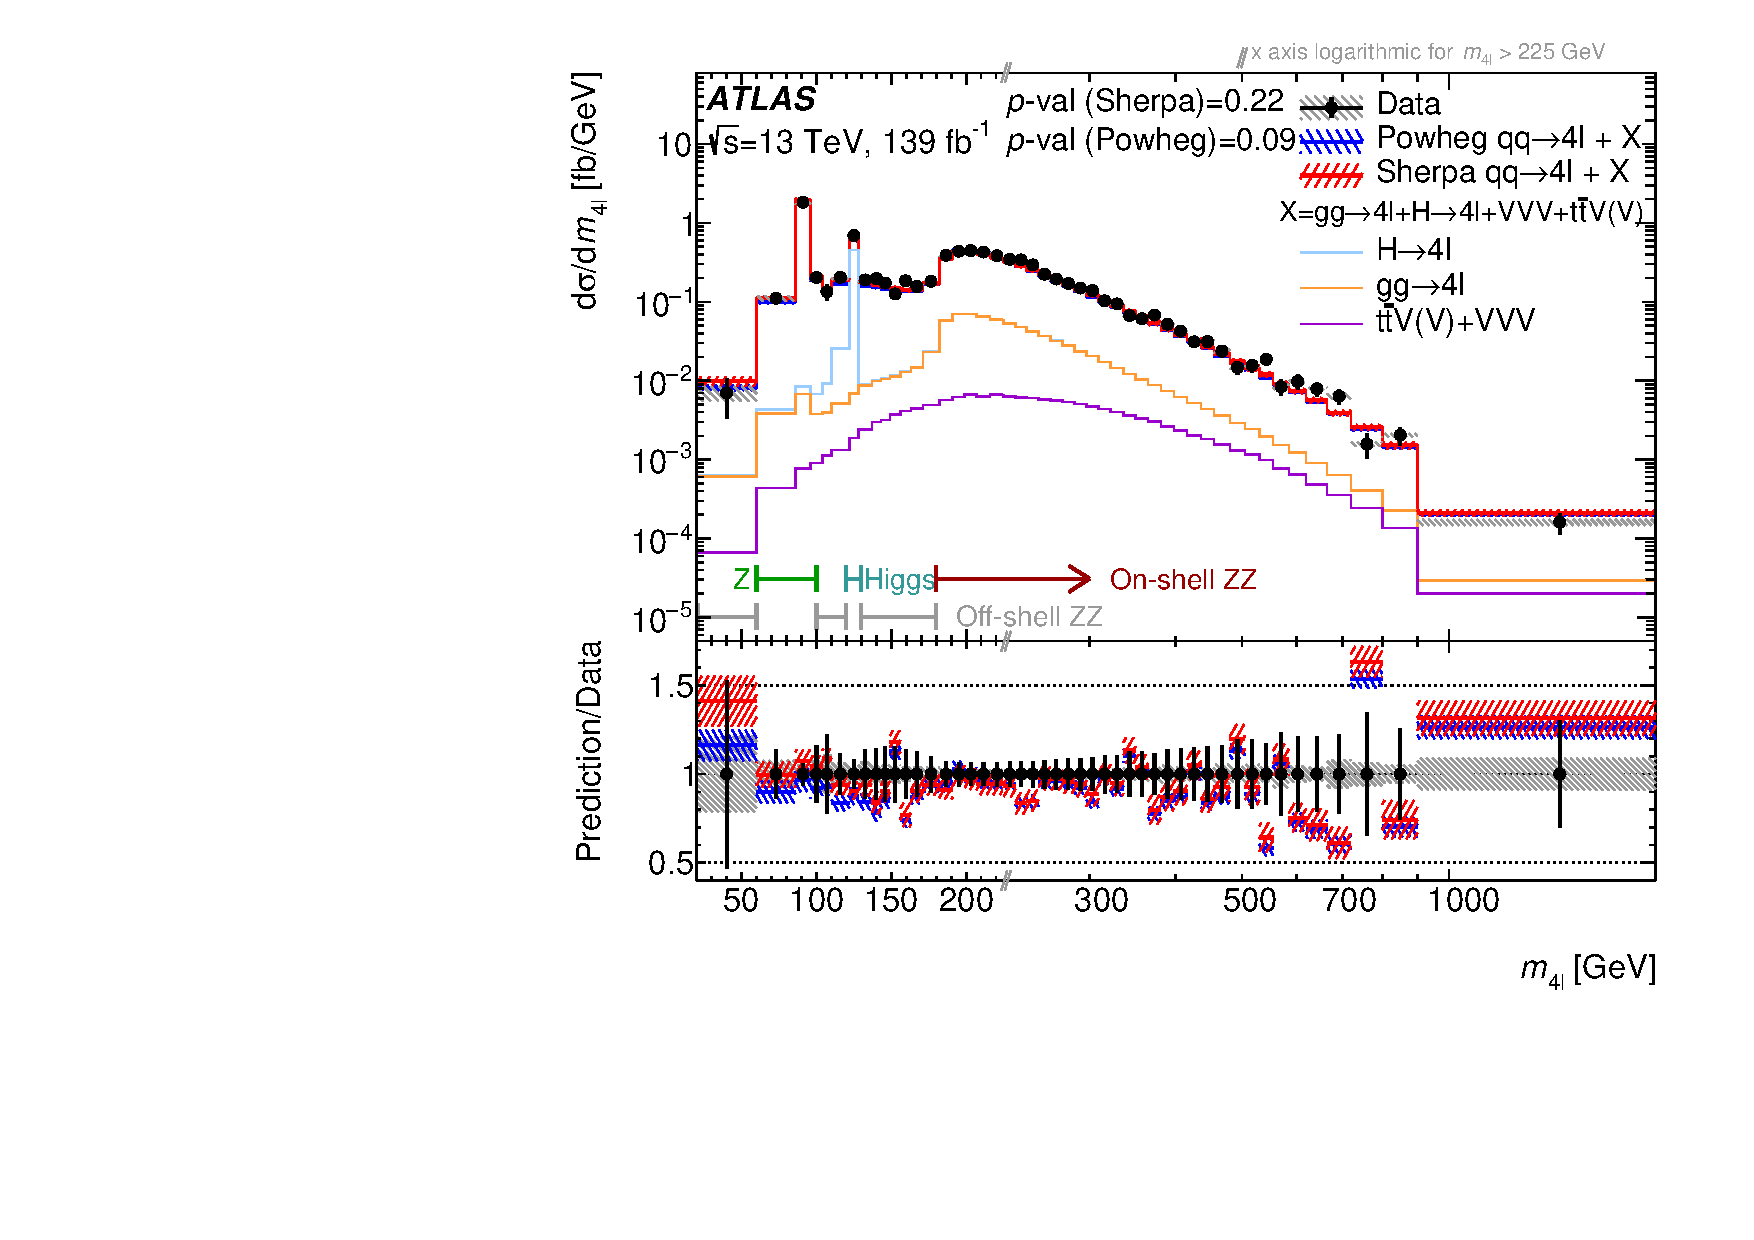
\includegraphics[width = 0.85\textwidth]{Figures/m4l/UnfoldedResults/linlog_Unfolded_Data_inclm4l.pdf} 
    \caption{Differential cross-section as a function of \mFourL. The measured data
  (black points)  are compared with the SM
  prediction using either \SHERPA{} (red, with red hashed
  band for the uncertainty) or \POWHEG{} + \pythia{} (blue,
  with blue hashed band for the uncertainty) to model the \qqFourL{} contribution. The error bars on the data points give the total uncertainty
  and the grey hashed band gives the systematic uncertainty. The
  breakdown of the contribution from different SM processes is also
  shown in successive stacked histograms.
  The short vertical lines terminating horizontal lines indicate the boundaries of the different
  \mFourL{} regions in which the other variables are measured.
  \Pvalue{}
  The
  lower panel shows the ratio of the SM predictions to the 
  data. The $x$-axis is on a linear scale until $\mFourL = 216$~\GeV,
  where it switches to a logarithmic scale. \label{fig:cross-sec-m4l}}
\end{figure}
In order to study the different \mFourL{} regions in more detail,  Figures~\ref{fig:mz1res} and~\ref{fig:mz2res} 
show the cross-section versus 
\mZOne{} and \mZTwo{} respectively in each region.
In the \HFourL{} region the contribution from Higgs production is
shown separately.

%% m4l vs pt4l
\begin{figure}[htb!]
    \begin{subfigure}{.49\textwidth}\centering
      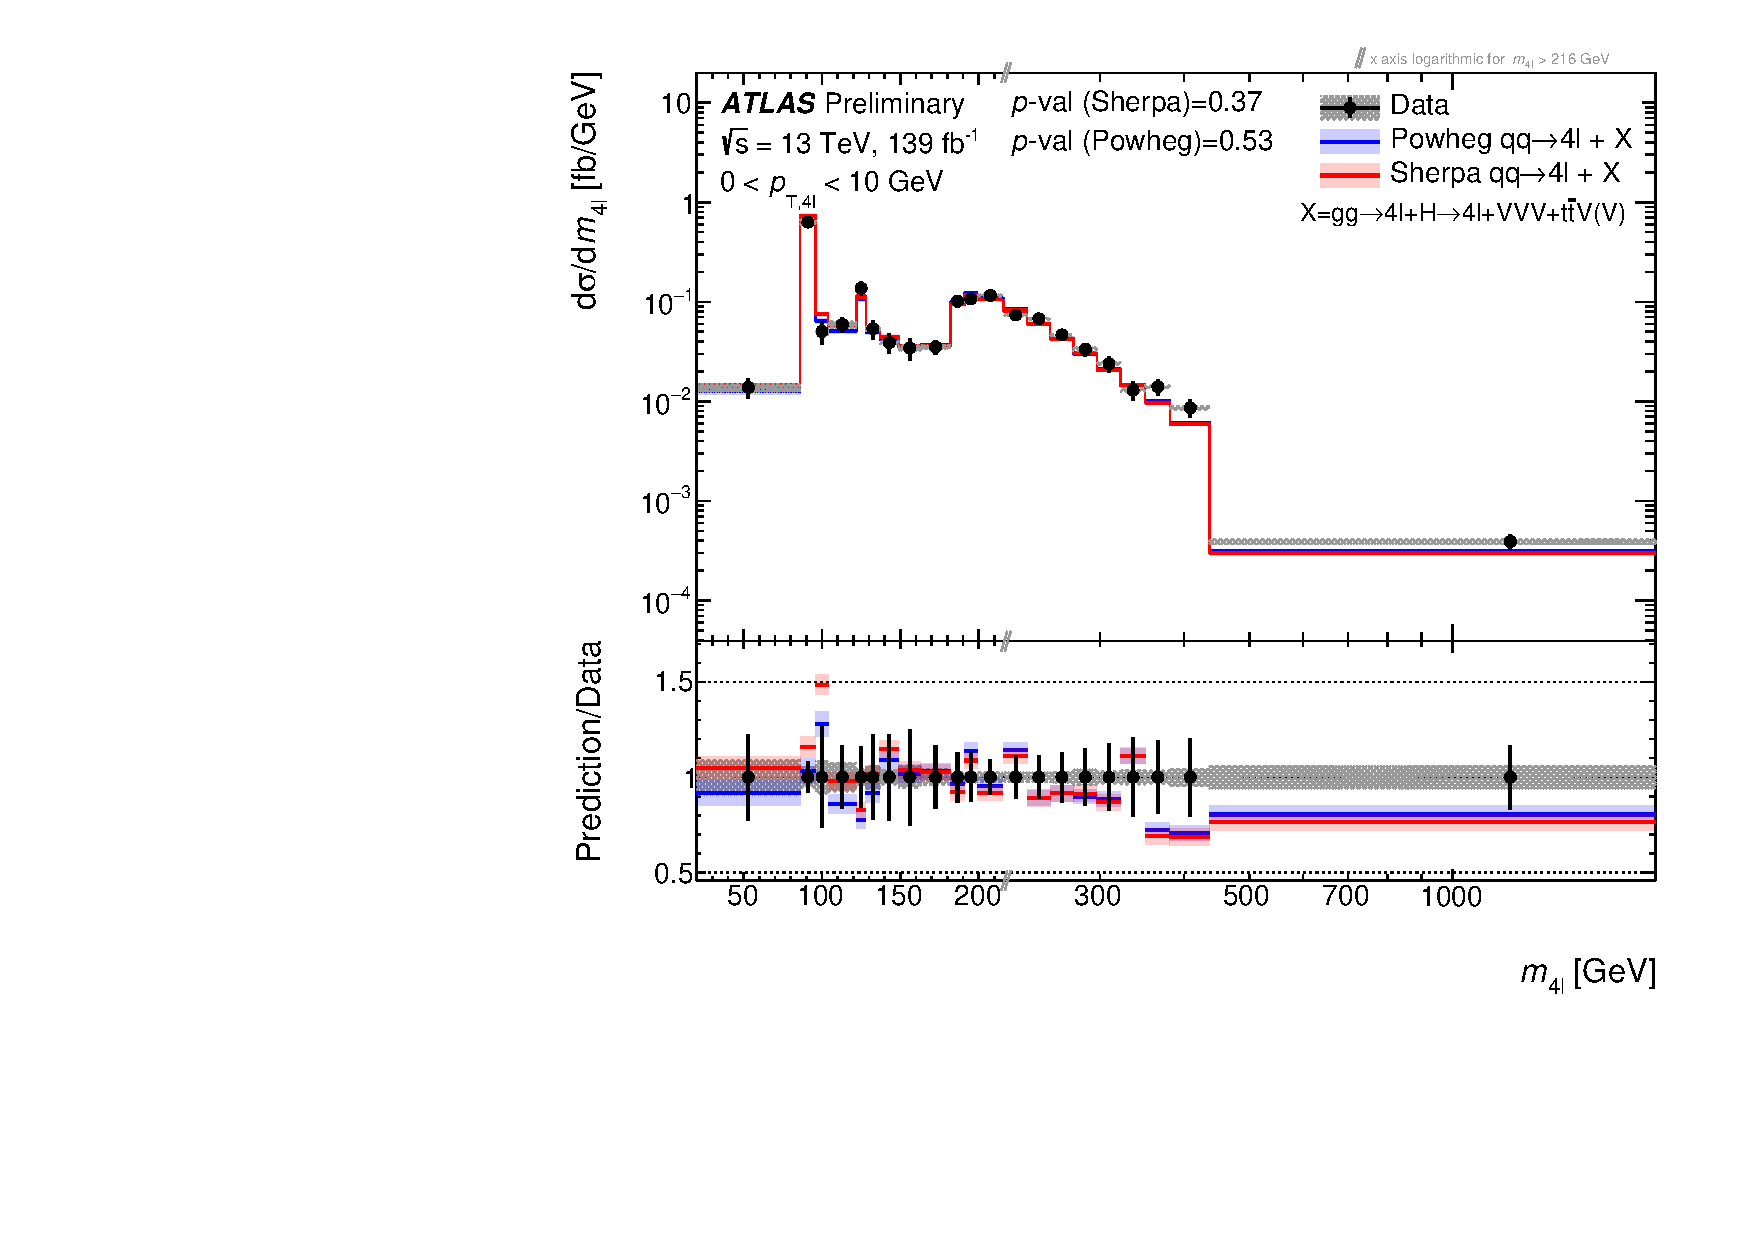
\includegraphics[width=.99\linewidth]{Figures/m4l/UnfoldedResults/linlog_Unfolded_Data_m4l_pt4l0-10.pdf}\caption{$\unit{0}{\GeV} <  \ptFourL  < \unit{10}{\GeV}$}\label{fig:sub-first}
    \end{subfigure}
    \begin{subfigure}{.49\textwidth}\centering
      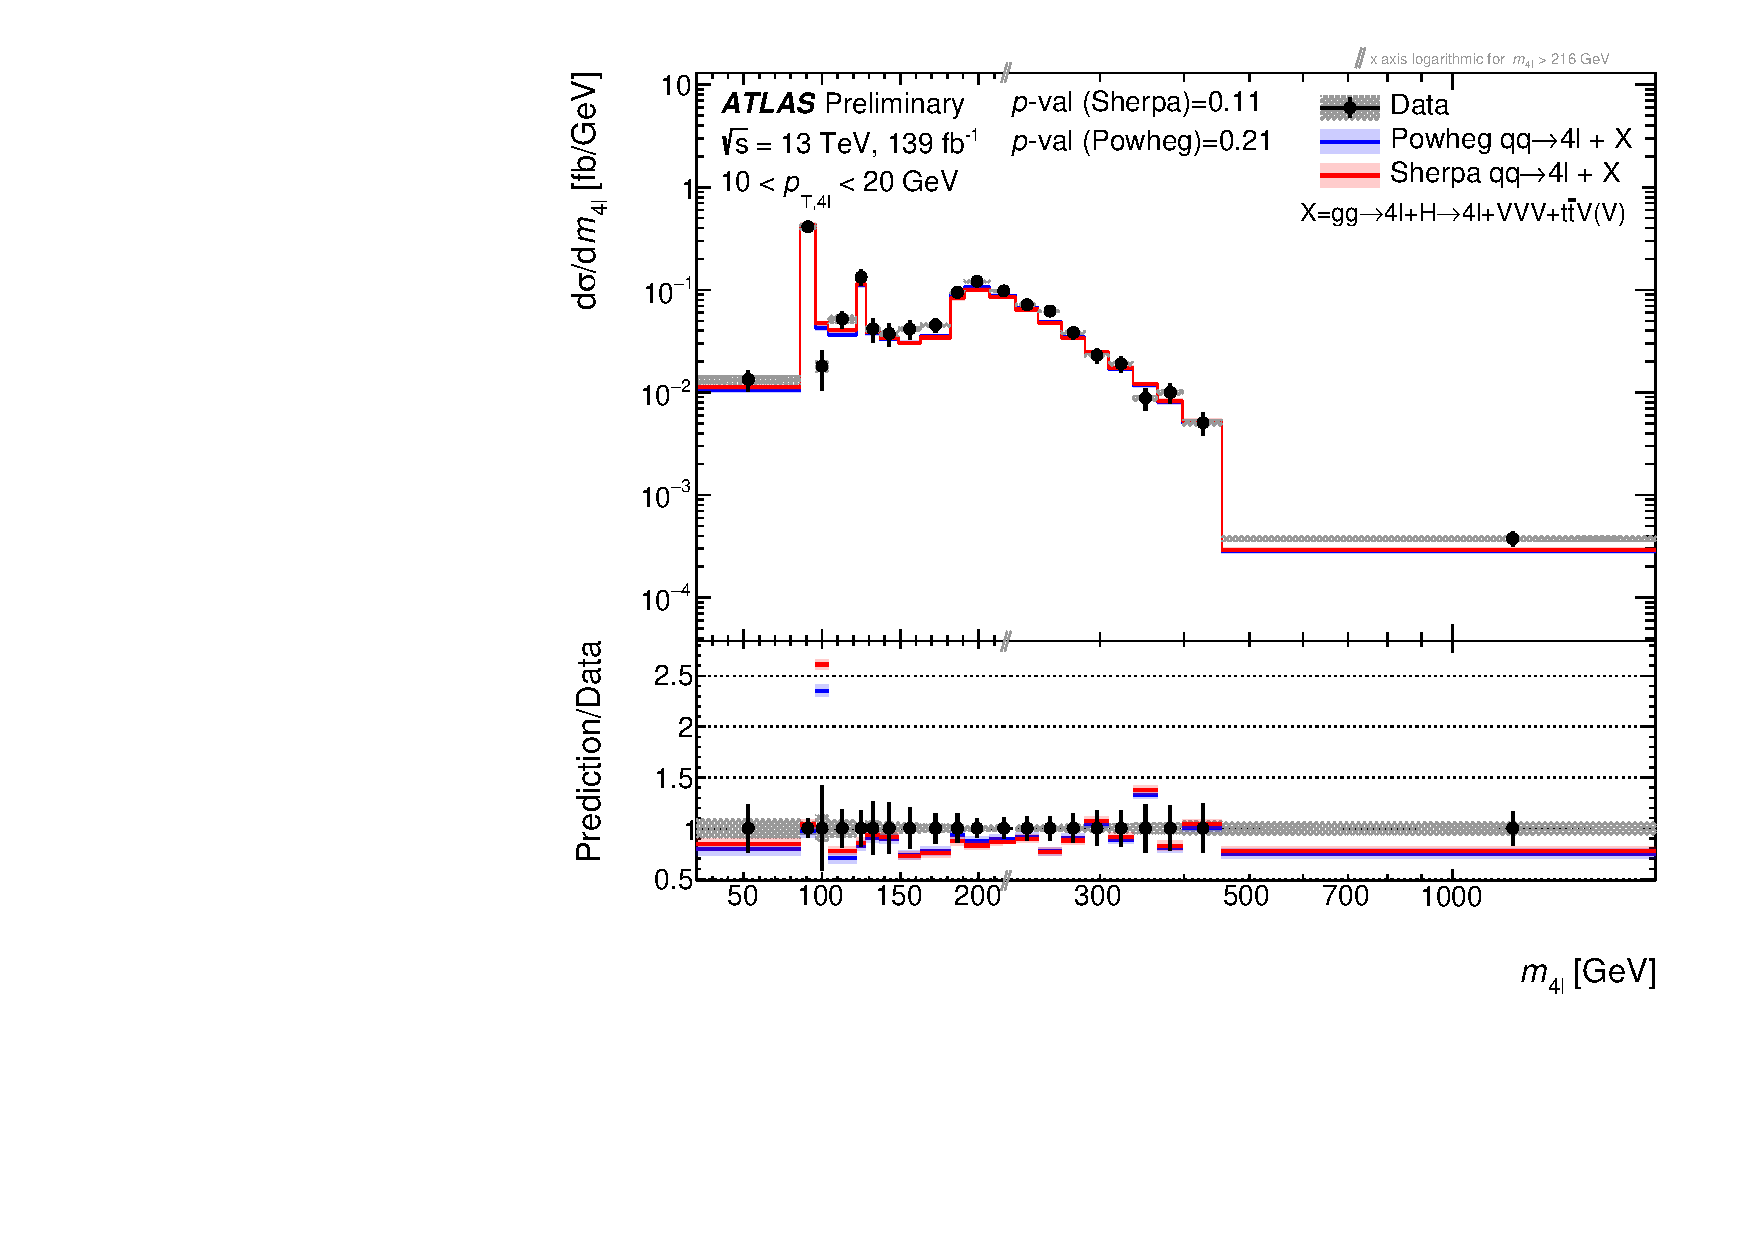
\includegraphics[width=.99\linewidth]{Figures/m4l/UnfoldedResults/linlog_Unfolded_Data_m4l_pt4l10-20.pdf} \caption{$\unit{10}{\GeV} <  \ptFourL  < \unit{20}{\GeV}$}\label{fig:sub-second}
    \end{subfigure}
    \begin{subfigure}{.49\textwidth}\centering
      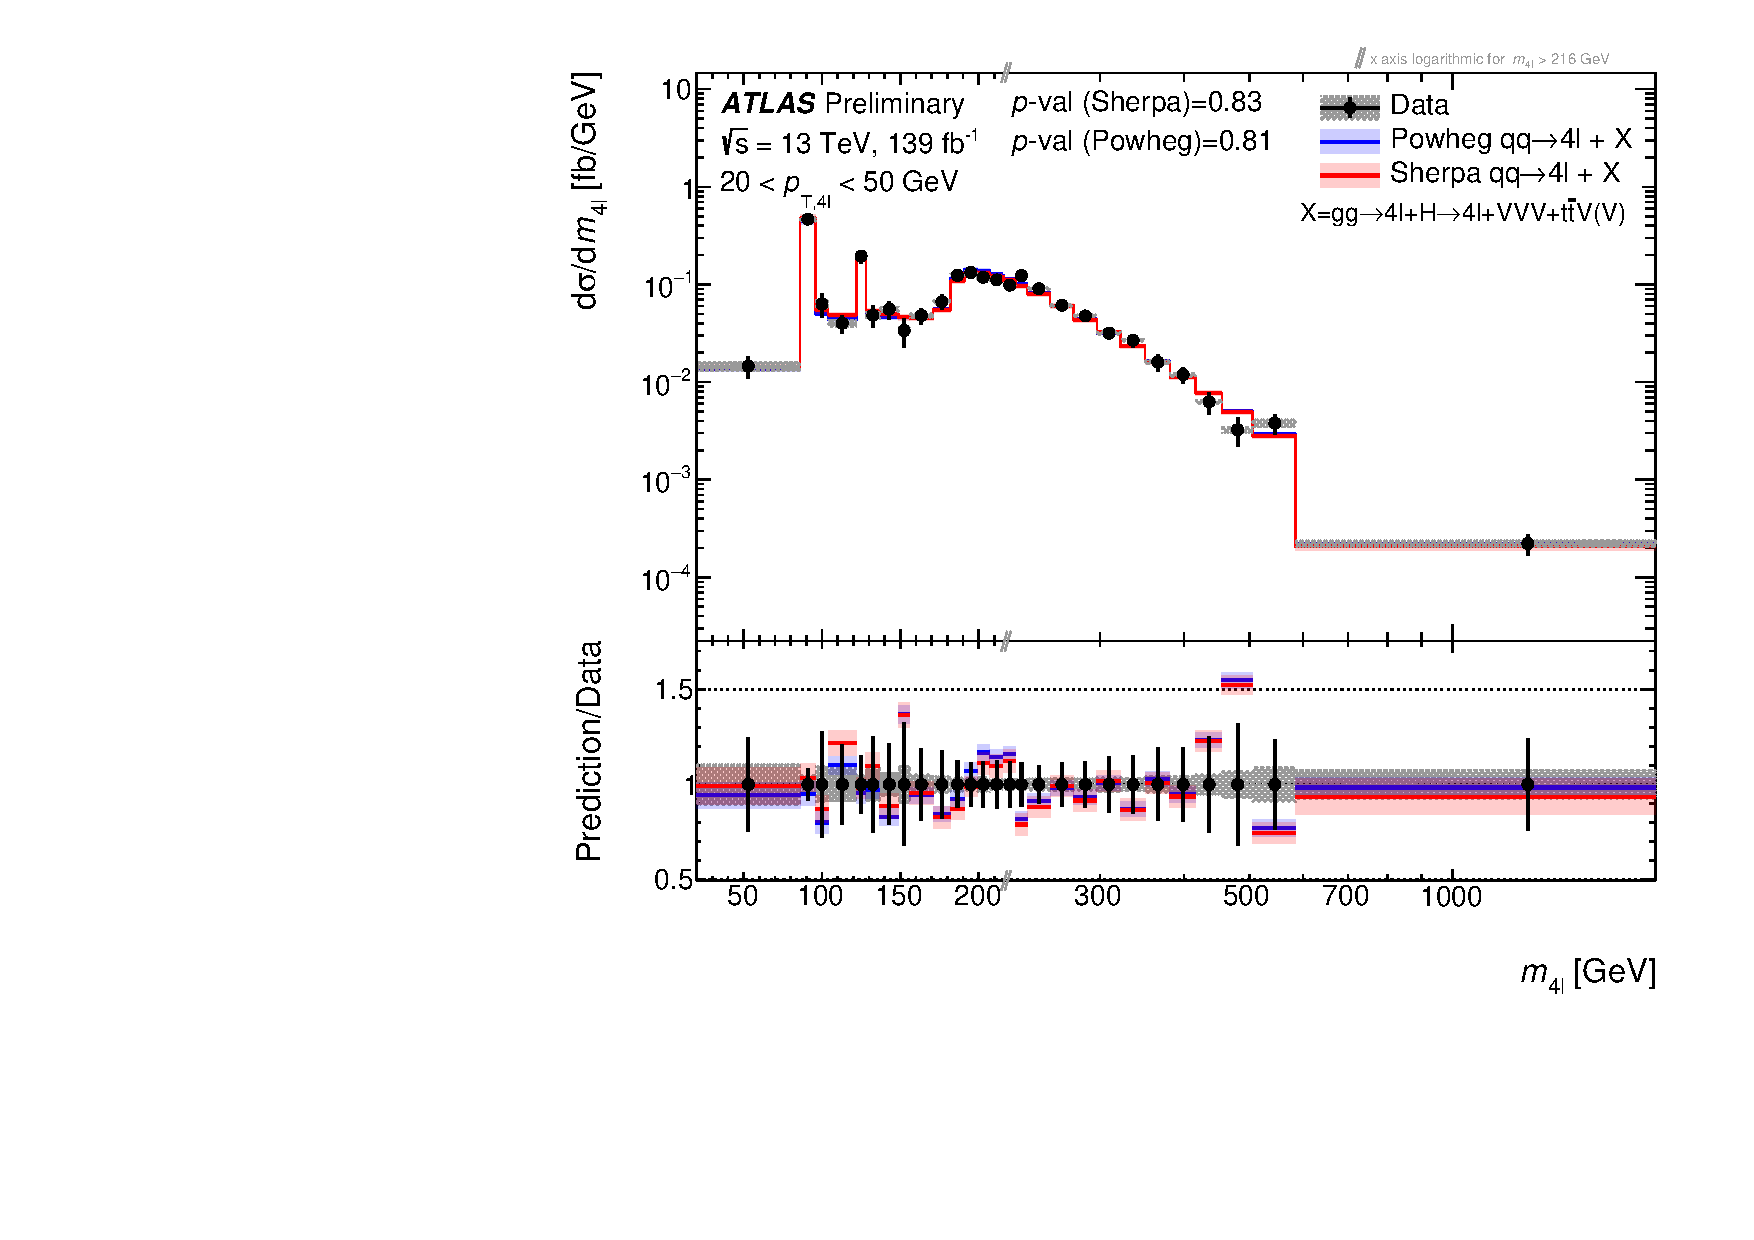
\includegraphics[width=.99\linewidth]{Figures/m4l/UnfoldedResults/linlog_Unfolded_Data_m4l_pt4l20-50.pdf}  \caption{$\unit{20}{\GeV} <  \ptFourL  < \unit{50}{\GeV}$}\label{fig:sub-third}
    \end{subfigure}
    \begin{subfigure}{.49\textwidth}\centering
      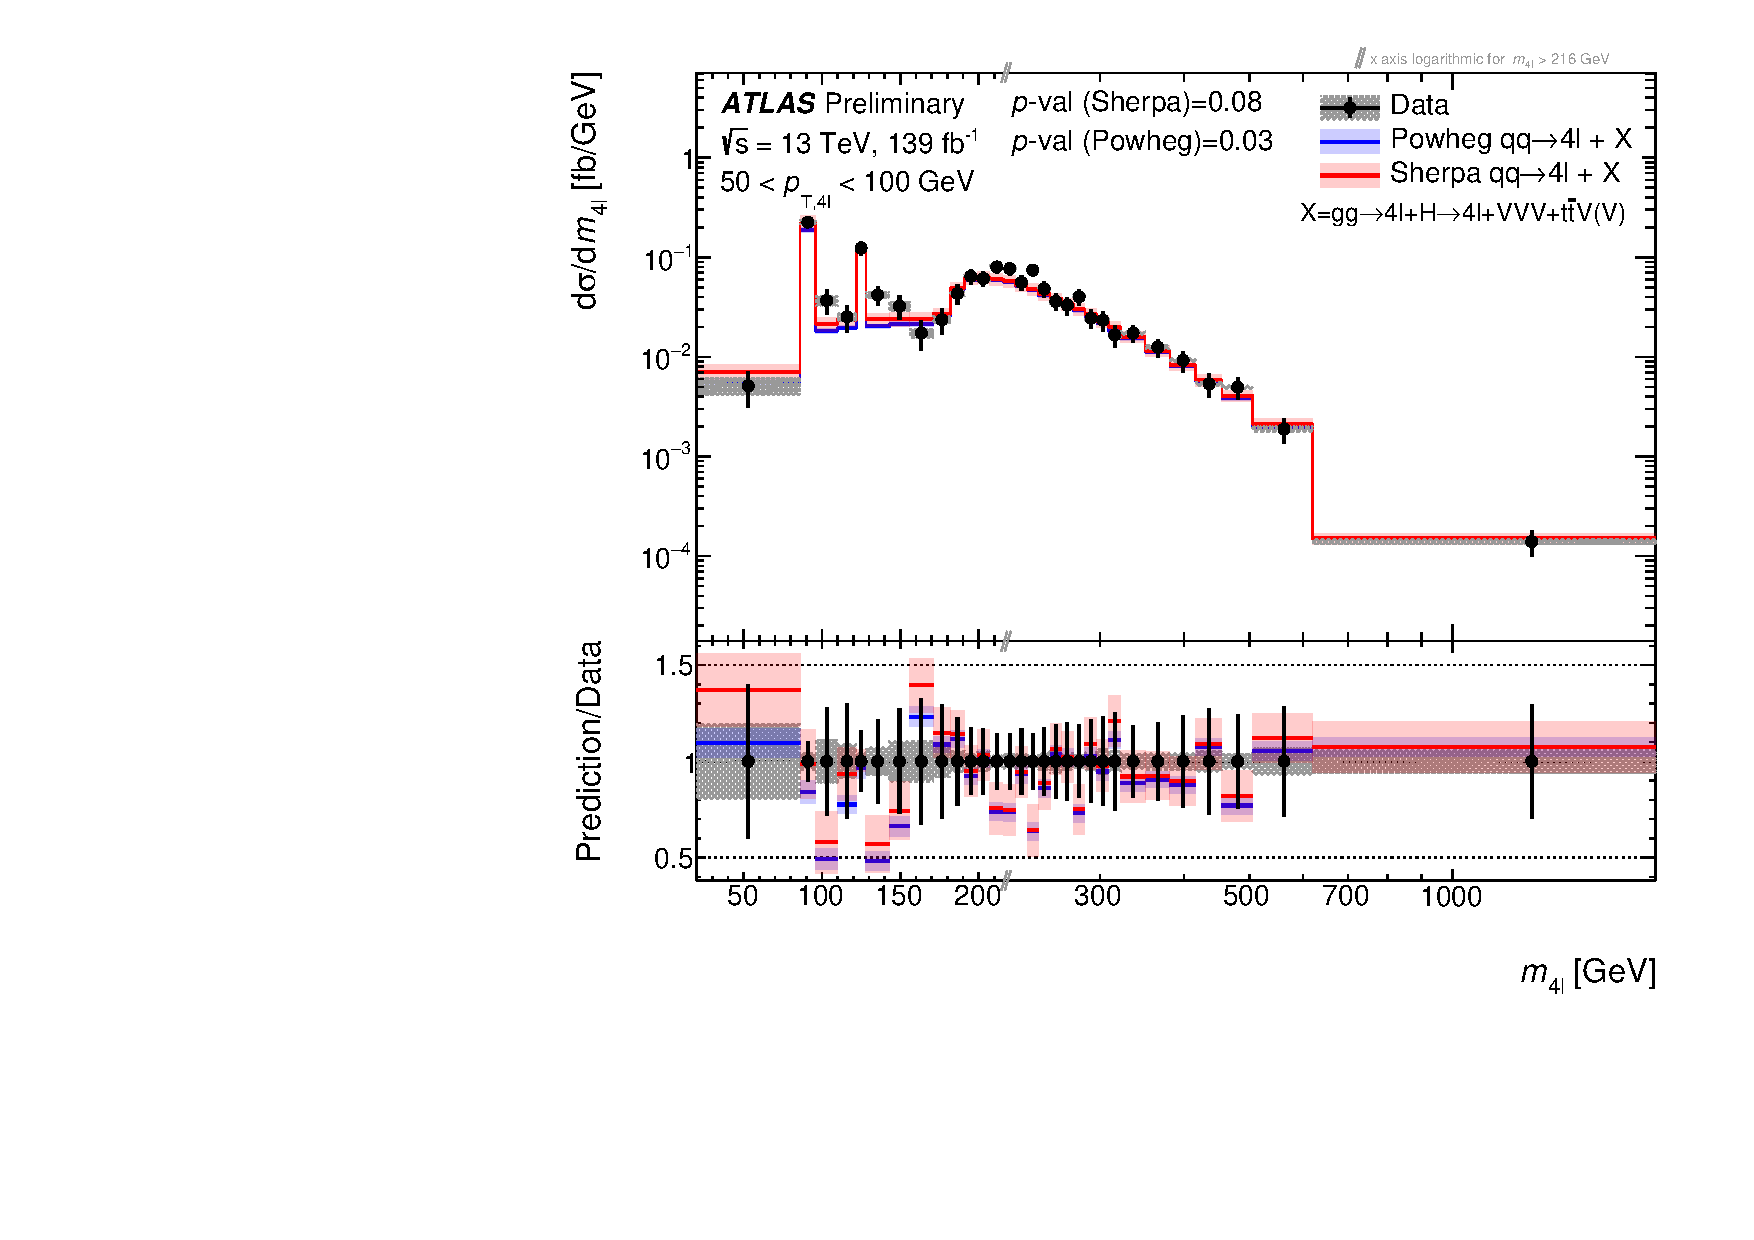
\includegraphics[width=.99\linewidth]{Figures/m4l/UnfoldedResults/linlog_Unfolded_Data_m4l_pt4l50-100.pdf}  \caption{$\unit{50}{\GeV} <  \ptFourL  < \unit{100}{\GeV}$}\label{fig:sub-fourth}
    \end{subfigure}
        \begin{subfigure}{.49\textwidth}\centering
      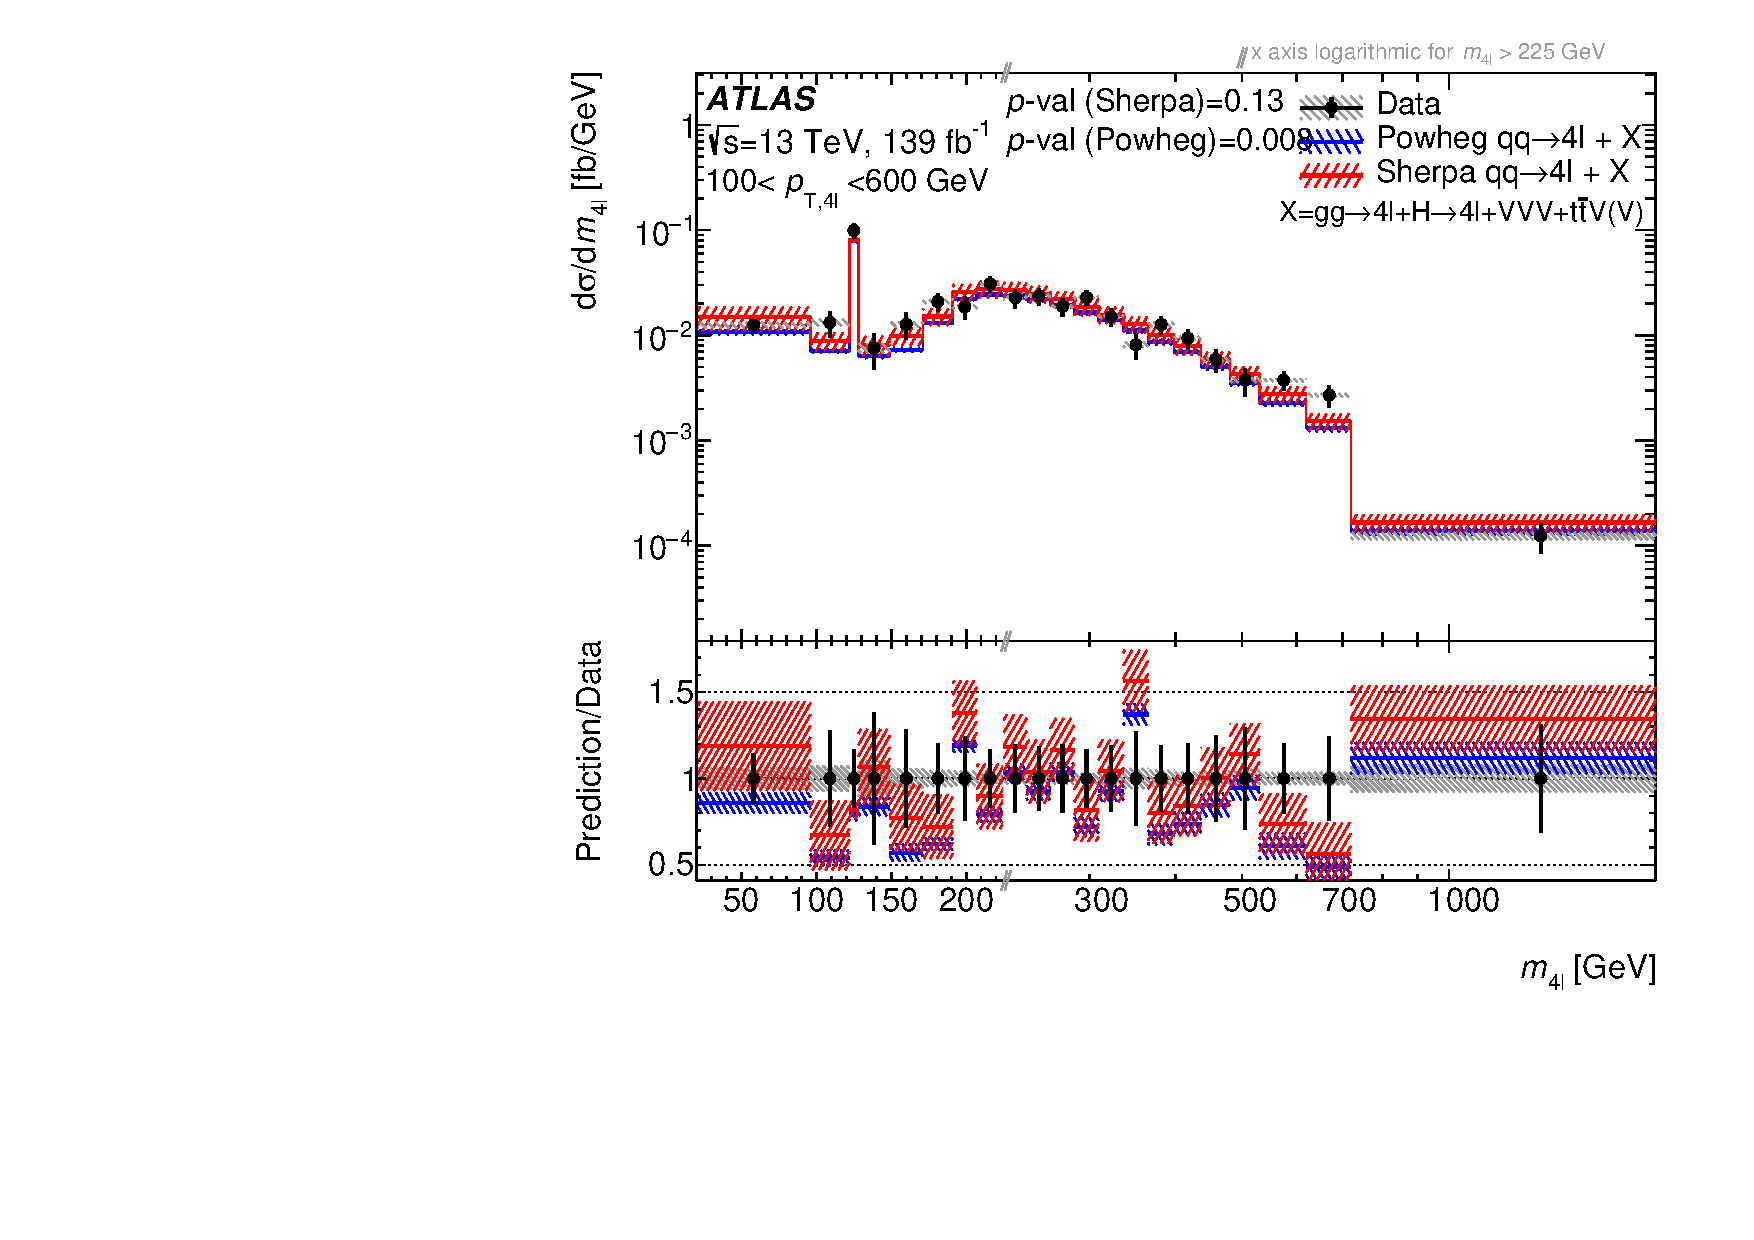
\includegraphics[width=.99\linewidth]{Figures/m4l/UnfoldedResults/linlog_Unfolded_Data_m4l_pt4l100-600.pdf}  \caption{$\unit{100}{\GeV} <  \ptFourL  < \unit{60 0}{\GeV}$}\label{fig:sub-fifth}
    \end{subfigure}
    \caption{Differential cross-section as a function of \mFourL{} in slices of \ptFourL{}. The measured data (black points) are  compared with the SM prediction using either \SHERPA{} (red, with red hashed band for the uncertainty) or \POWHEG{} + \pythia{} (blue, with blue hashed band for the uncertainty) to model the \qqFourL{} contribution. The error bars on the data points give the total uncertainty and the grey hashed band gives the systematic uncertainty. \Pvalue{} The  lower panel shows the ratio of the SM predictions to the data.}
    \label{fig:m4l_pt4l}
\end{figure}

%% m4l vs y4l
\begin{figure}[htb!]
    \begin{subfigure}{.49\textwidth}\centering
      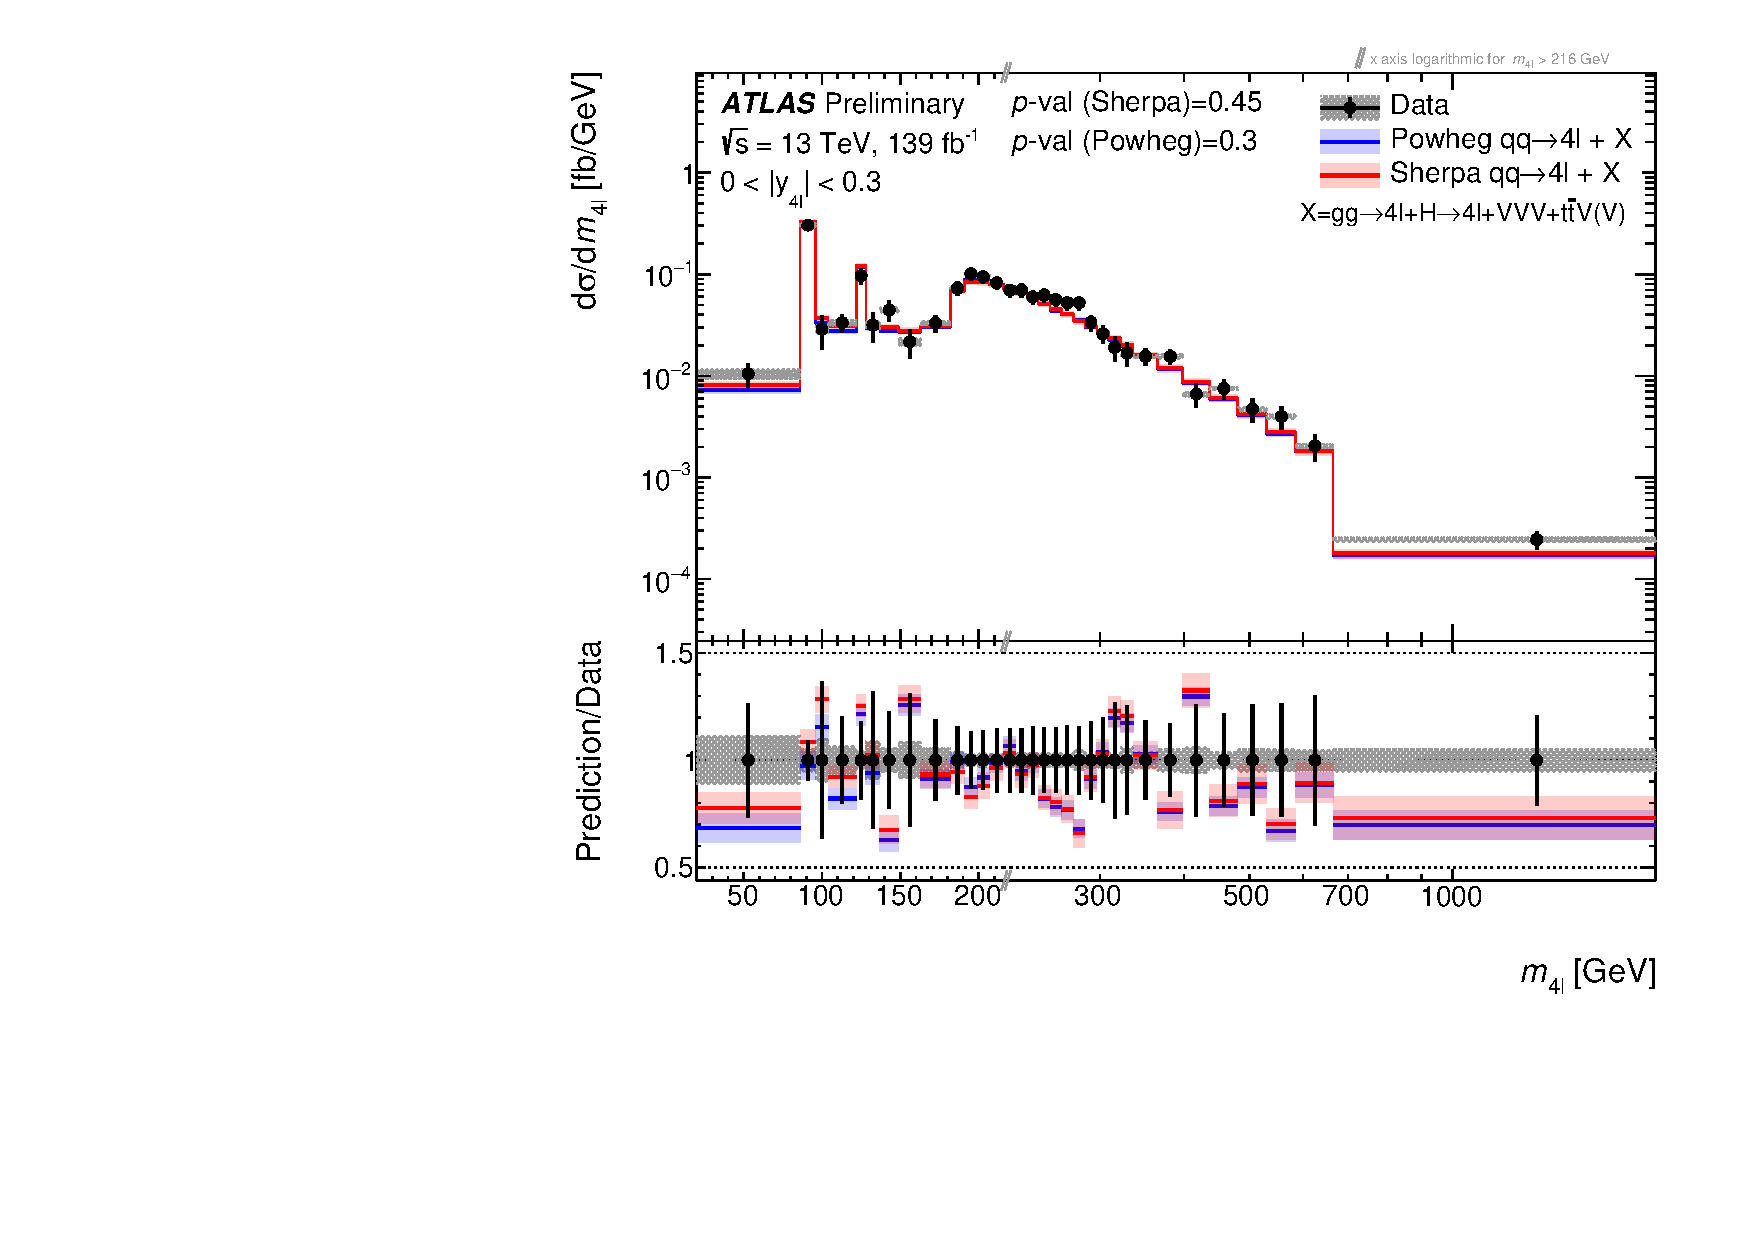
\includegraphics[width=.99\linewidth]{Figures/m4l/UnfoldedResults/linlog_Unfolded_Data_m4l_y4l0-0dot3.pdf}\caption{0 < \yFourL{} < 0.3}\label{fig:sub-first}
    \end{subfigure}
    \begin{subfigure}{.49\textwidth}\centering
      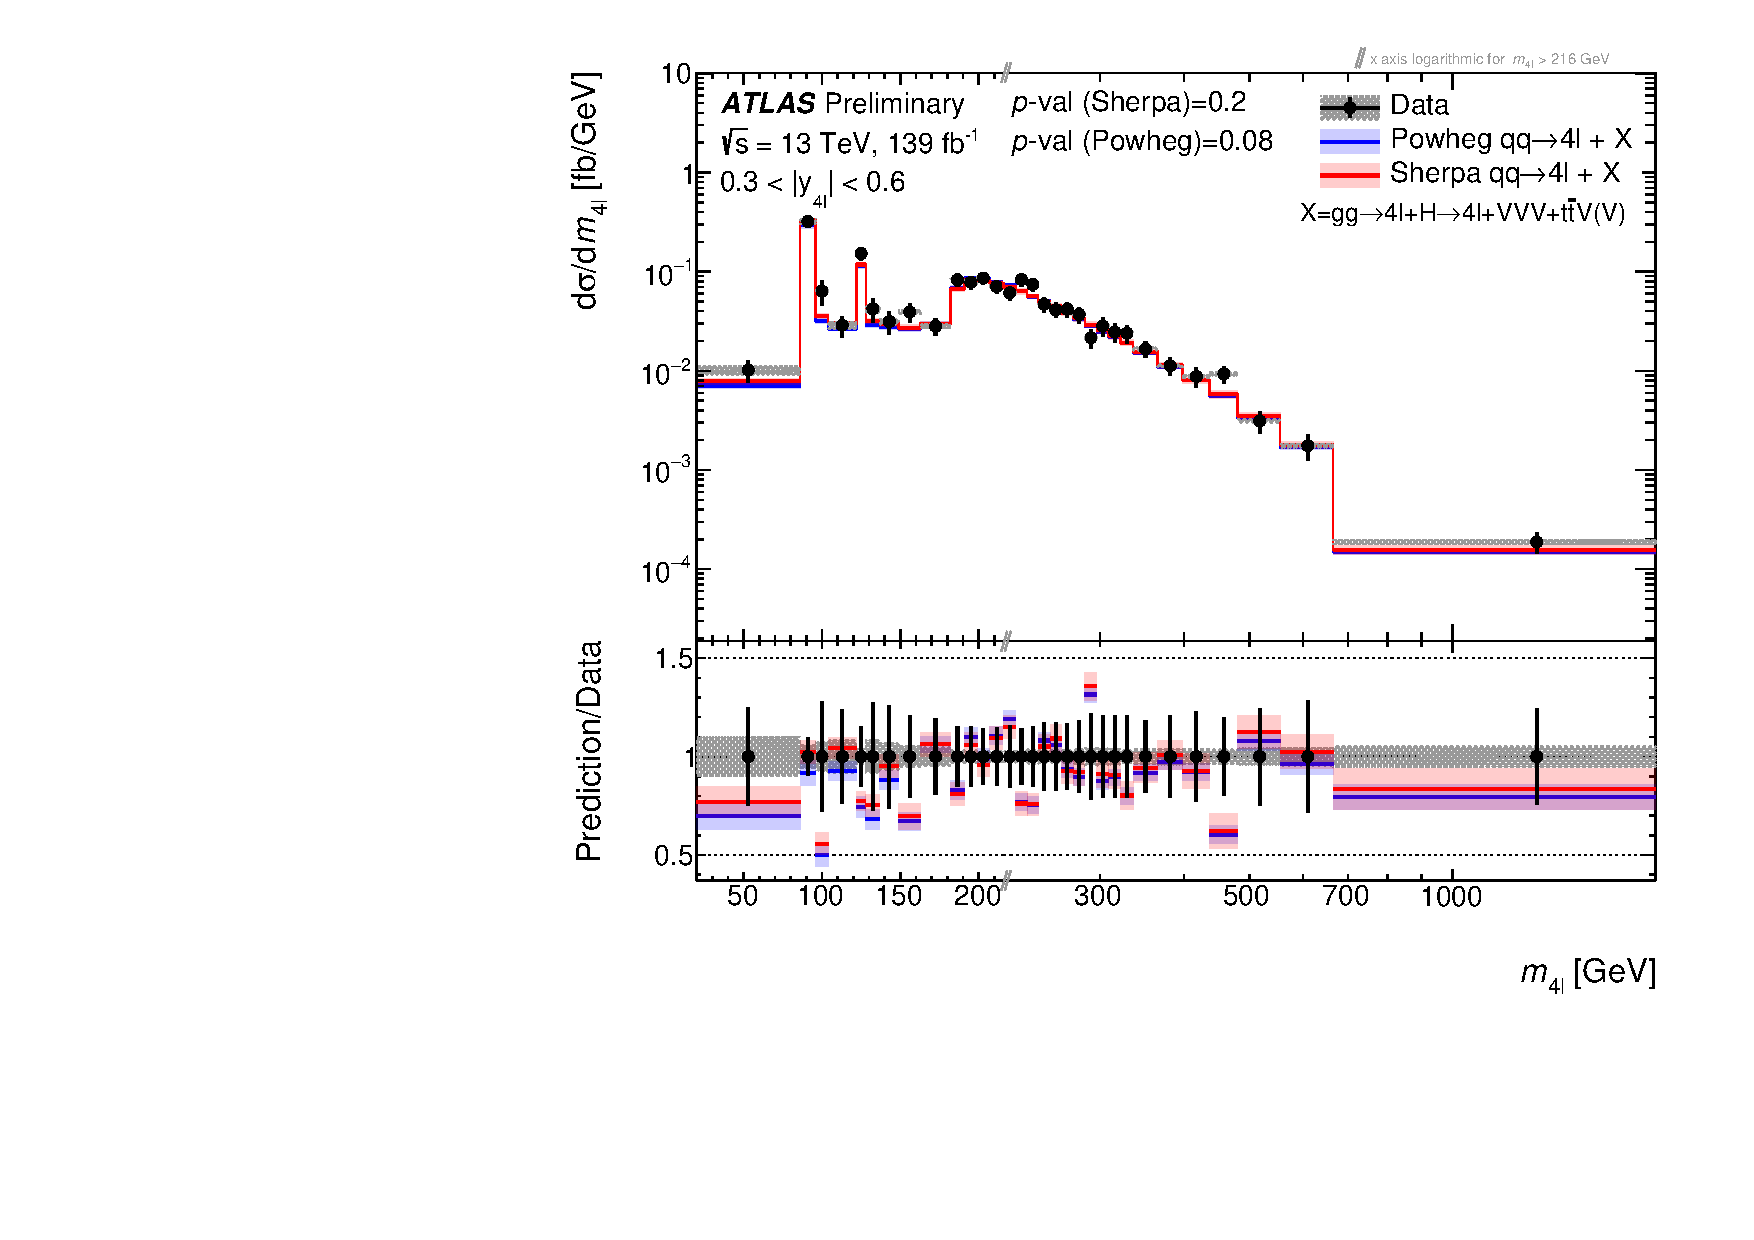
\includegraphics[width=.99\linewidth]{Figures/m4l/UnfoldedResults/linlog_Unfolded_Data_m4l_y4l0dot3-0dot6.pdf} \caption{0.3 < \yFourL{} < 0.6}\label{fig:sub-second}
    \end{subfigure}
    \begin{subfigure}{.49\textwidth}\centering
      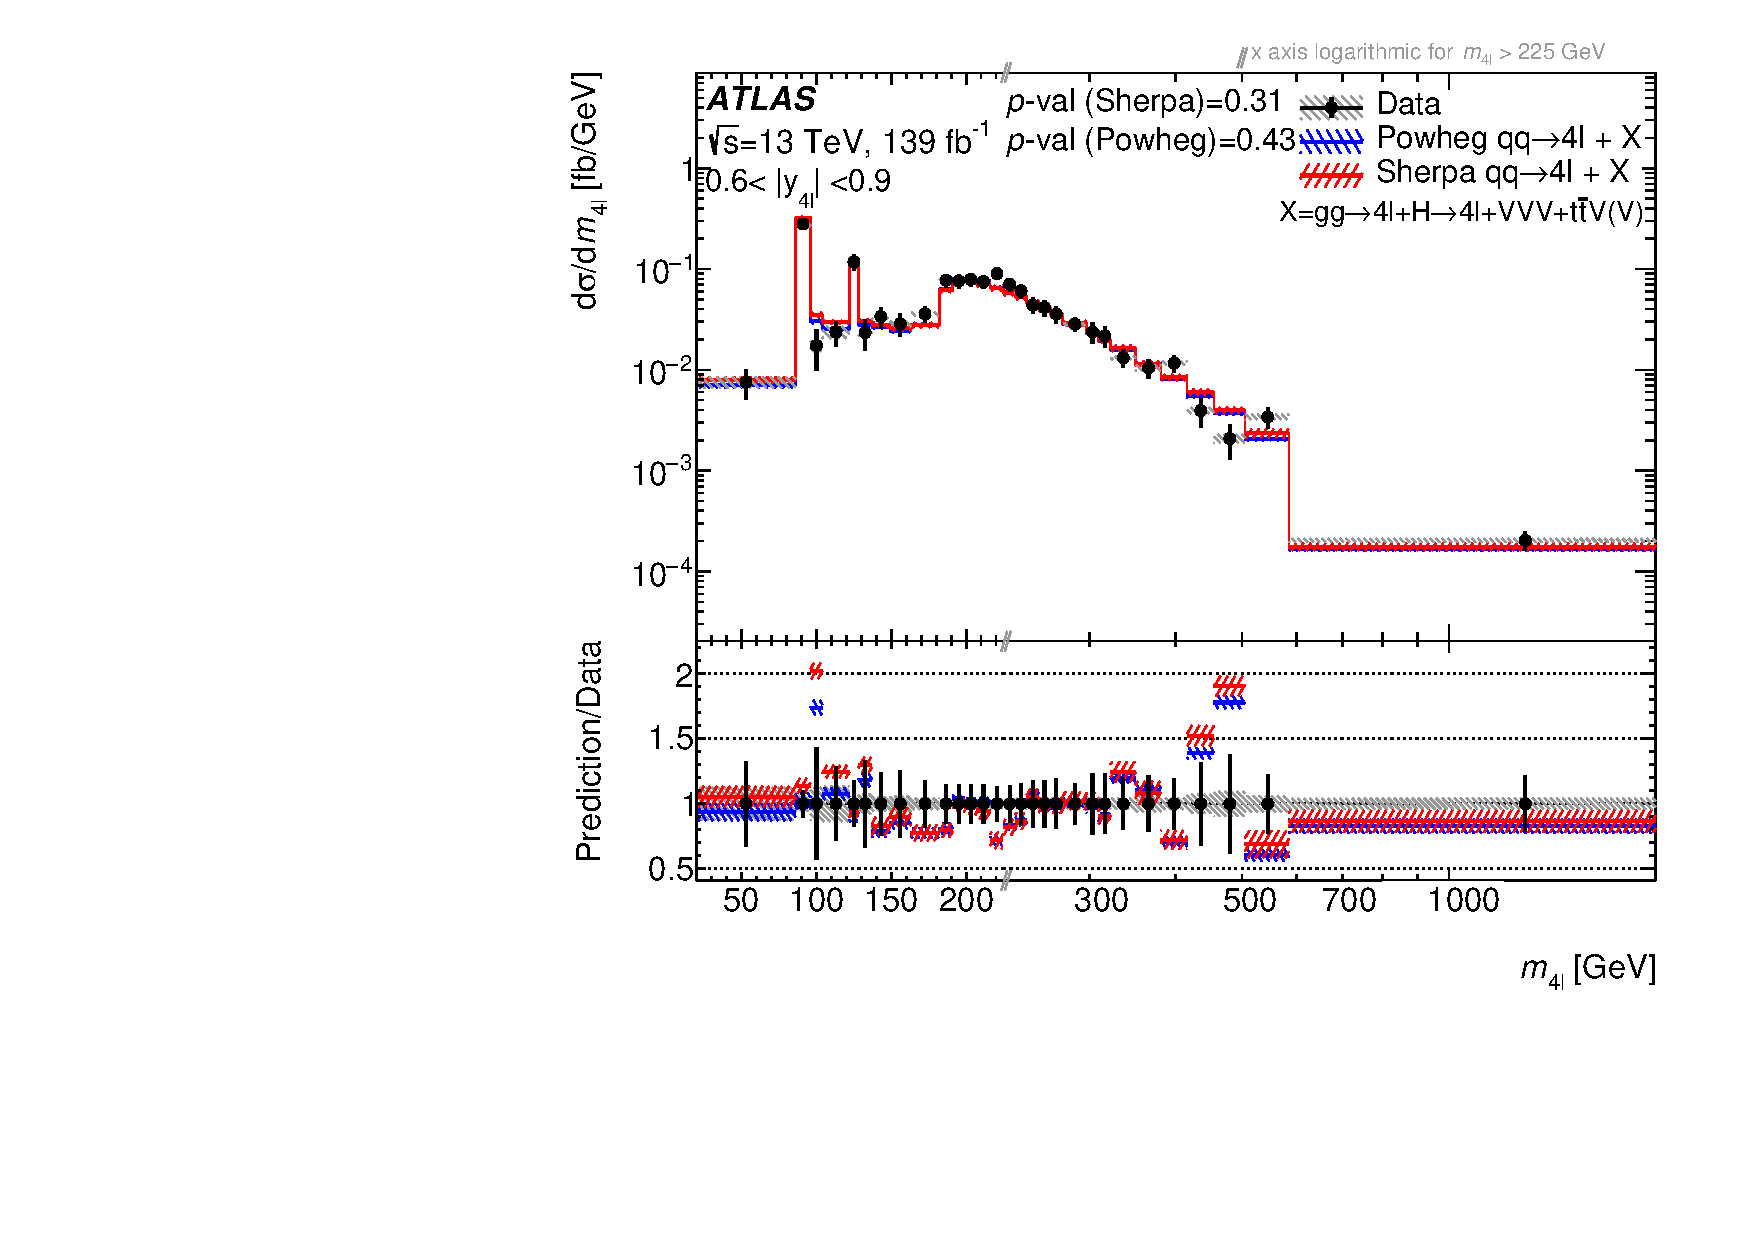
\includegraphics[width=.99\linewidth]{Figures/m4l/UnfoldedResults/linlog_Unfolded_Data_m4l_y4l0dot6-0dot9.pdf}  \caption{0.6 < \yFourL{} < 0.9}\label{fig:sub-third}
    \end{subfigure}
    \begin{subfigure}{.49\textwidth}\centering
      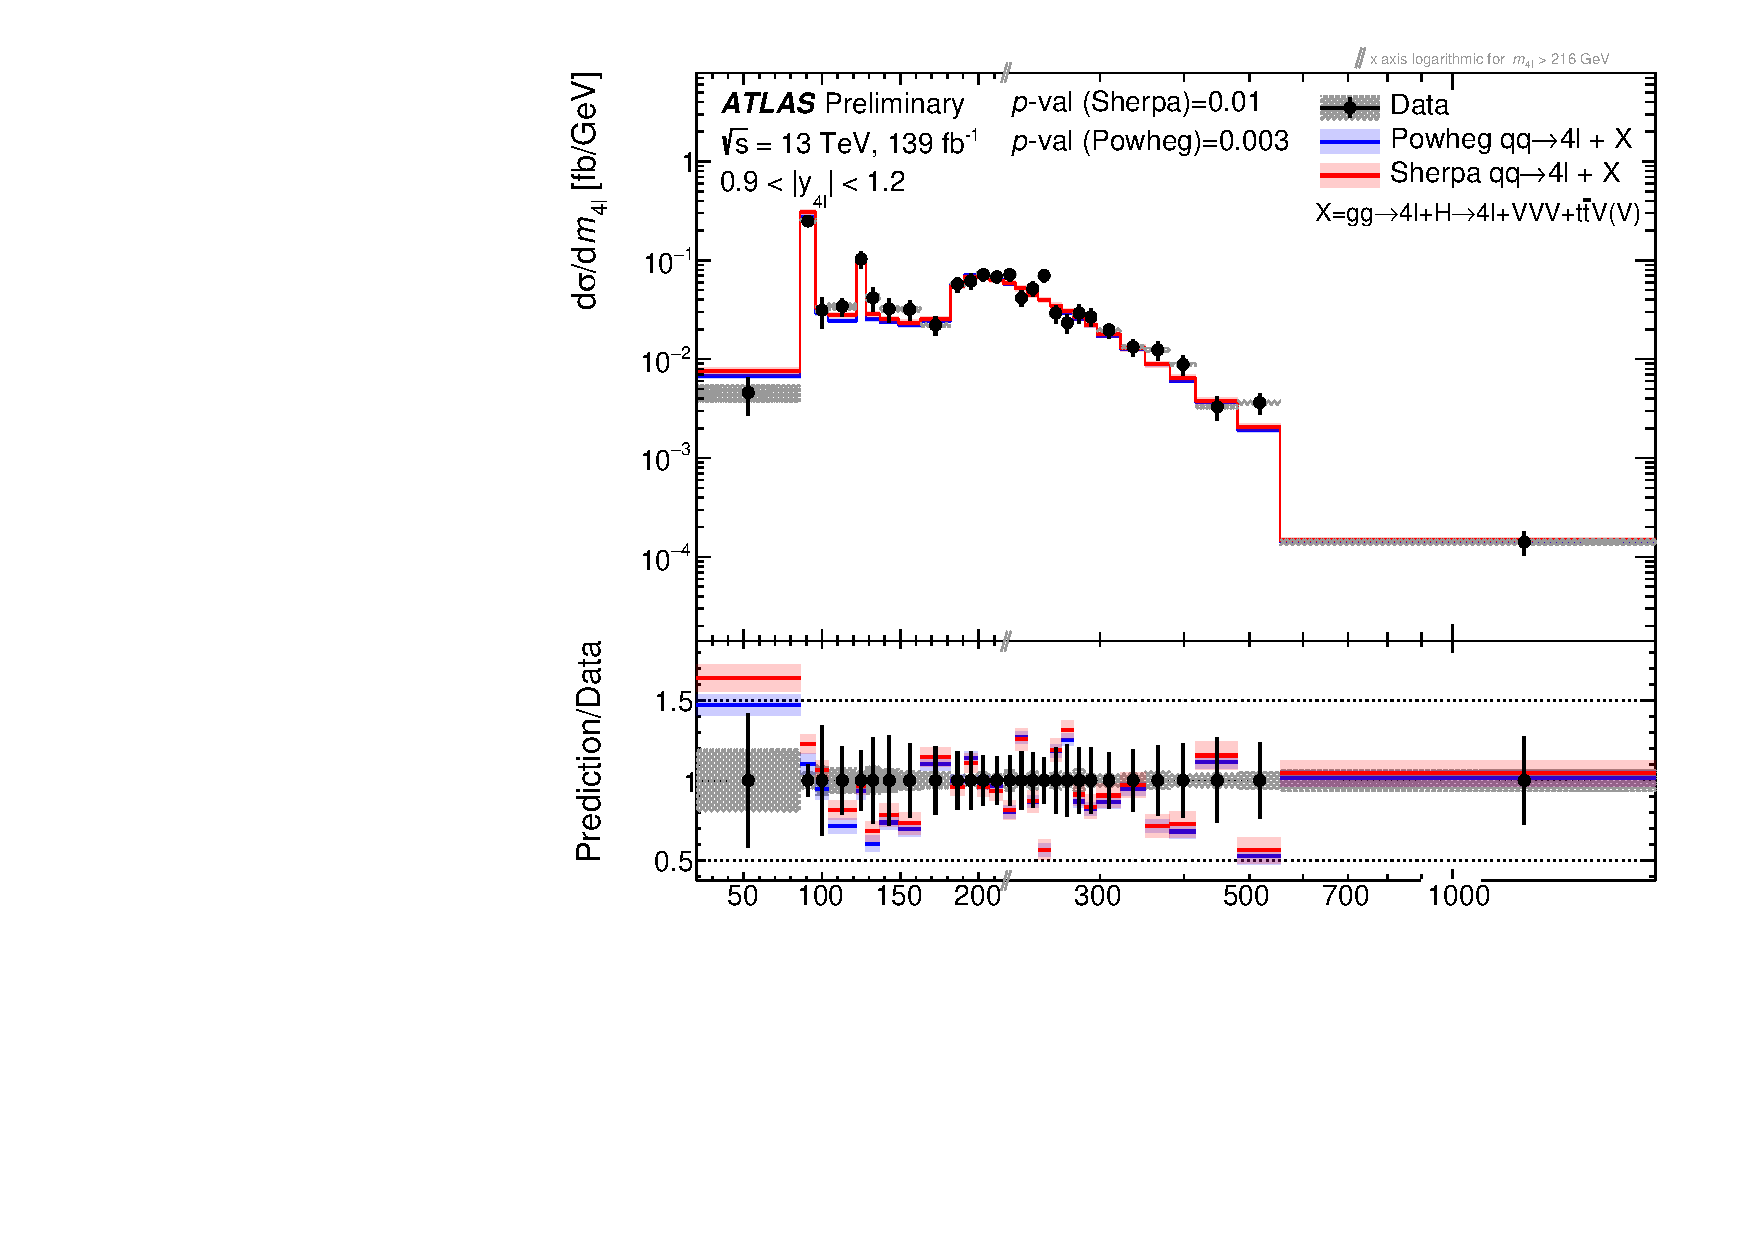
\includegraphics[width=.99\linewidth]{Figures/m4l/UnfoldedResults/linlog_Unfolded_Data_m4l_y4l0dot9-1dot2.pdf}  \caption{0.9 < \yFourL{} < 1.2}\label{fig:sub-fourth}
    \end{subfigure}
        \begin{subfigure}{.49\textwidth}\centering
      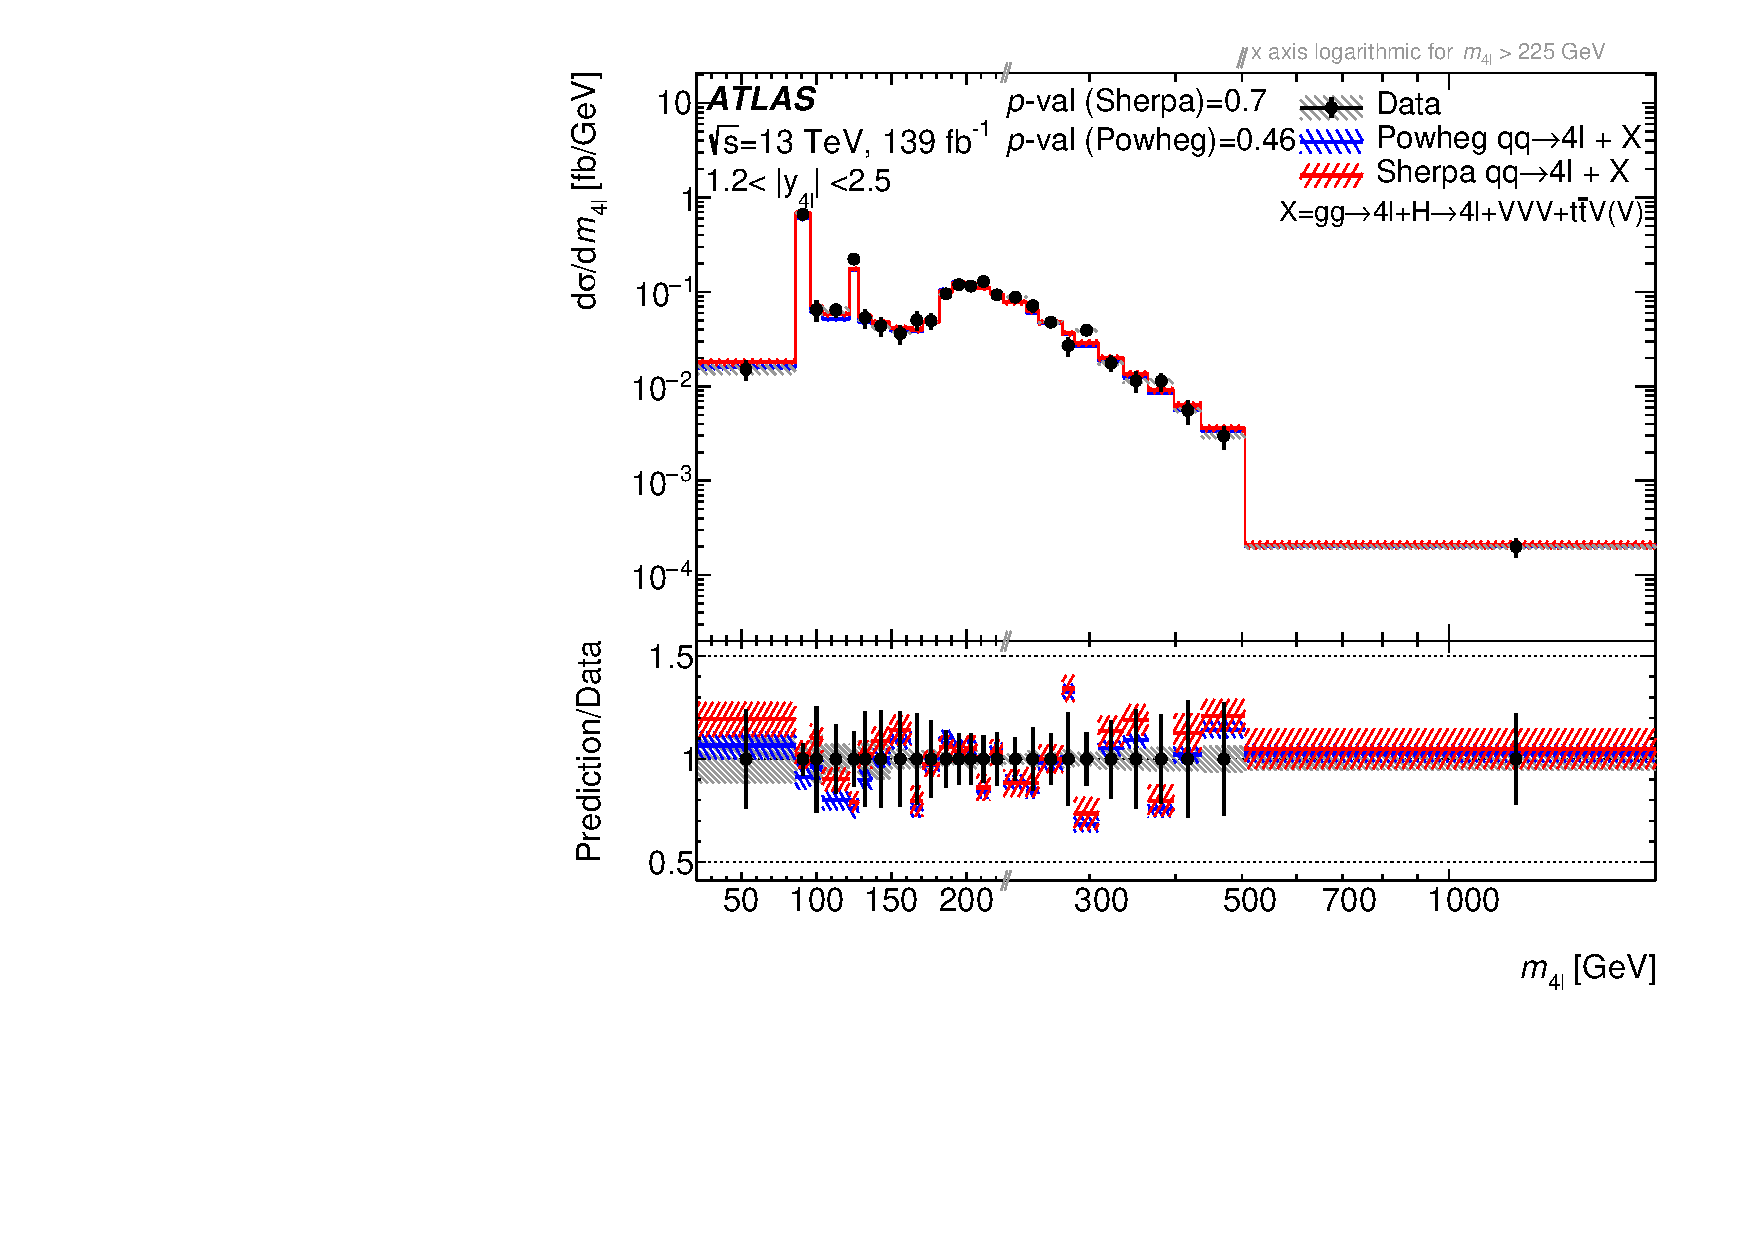
\includegraphics[width=.99\linewidth]{Figures/m4l/UnfoldedResults/linlog_Unfolded_Data_m4l_y4l1dot2-2dot5.pdf}  \caption{1.2 < \yFourL{} < 2.5}\label{fig:sub-fifth}
    \end{subfigure}
    \caption{Differential cross-section as a function of \mFourL{} in slices of \yFourL{}. The measured data (black points) are  compared with the SM prediction using either \SHERPA{} (red, with red hashed band for the uncertainty) or \POWHEG{} + \pythia{} (blue, with blue hashed band for the uncertainty) to model the \qqFourL{} contribution. The error bars on the data points give the total uncertainty and the grey hashed band gives the systematic uncertainty. \Pvalue{} The  lower panel shows the ratio of the SM predictions to the data.}
    \label{fig:m4l_y4l}
\end{figure}

%% m4l vs flavour
\begin{figure}[htb!]
    \begin{subfigure}{.49\textwidth}\centering
      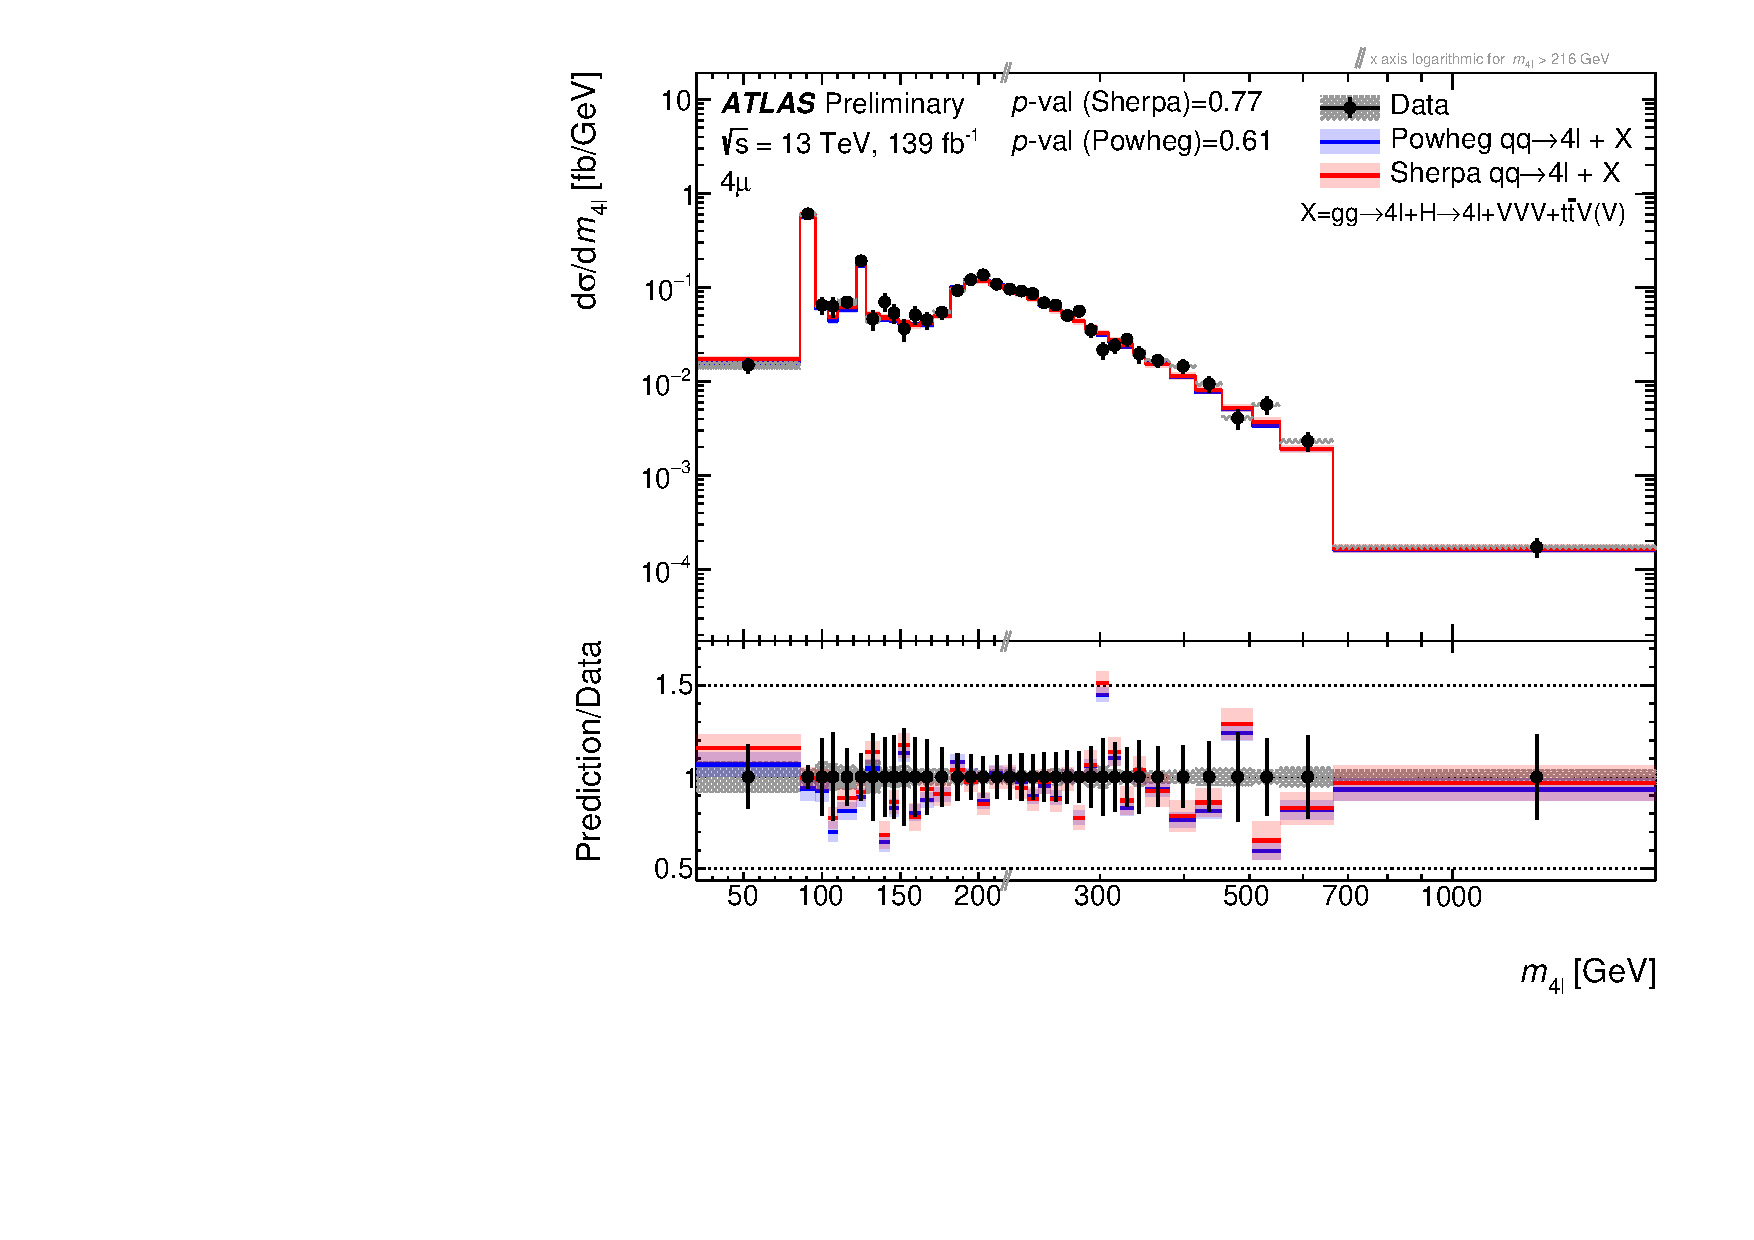
\includegraphics[width=.99\linewidth]{Figures/m4l/UnfoldedResults/linlog_Unfolded_Data_m4l_event_type4mu.pdf}\caption{$4\mu$ channel}\label{fig:sub-first}
    \end{subfigure}
    \begin{subfigure}{.49\textwidth}\centering
      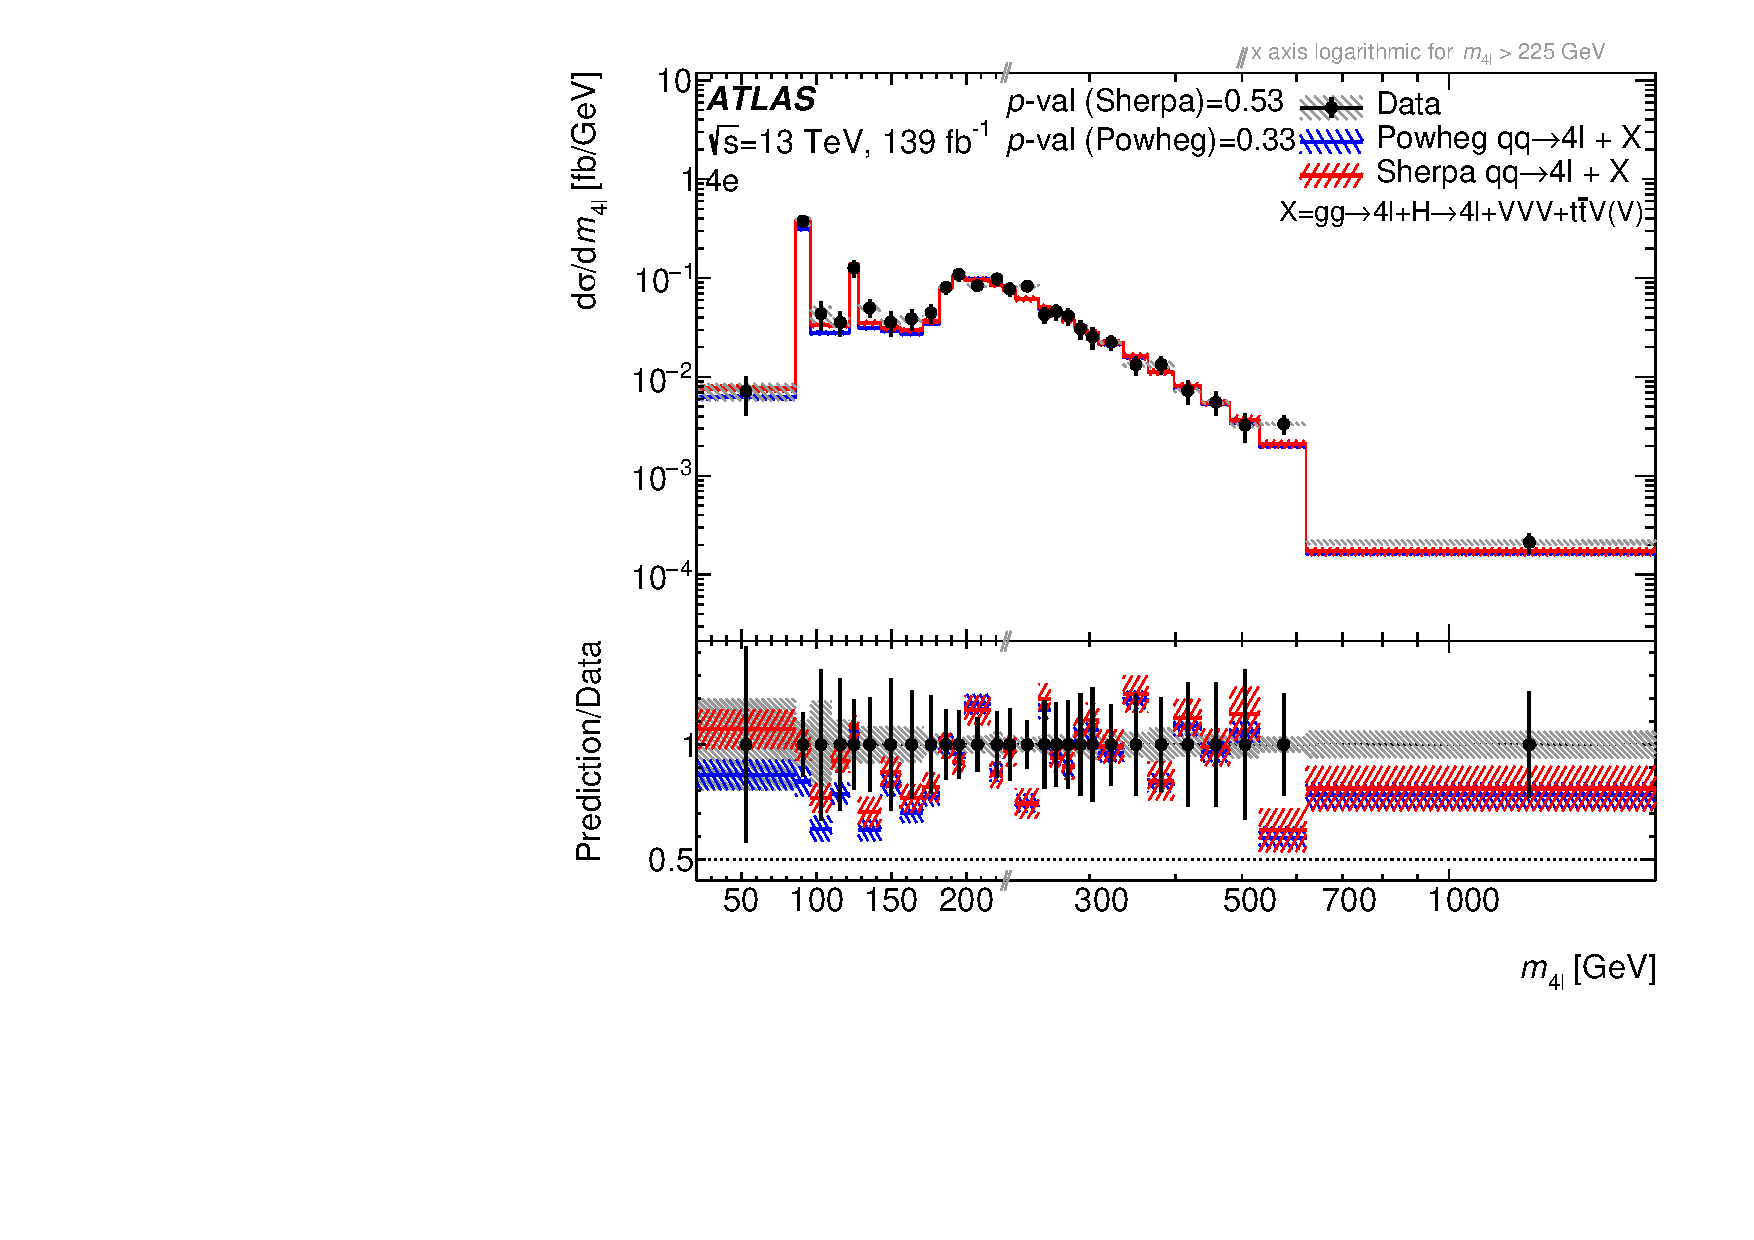
\includegraphics[width=.99\linewidth]{Figures/m4l/UnfoldedResults/linlog_Unfolded_Data_m4l_event_type4e.pdf} \caption{$4e$ channel}\label{fig:sub-second}
    \end{subfigure}
    \begin{subfigure}{.49\textwidth}\centering
      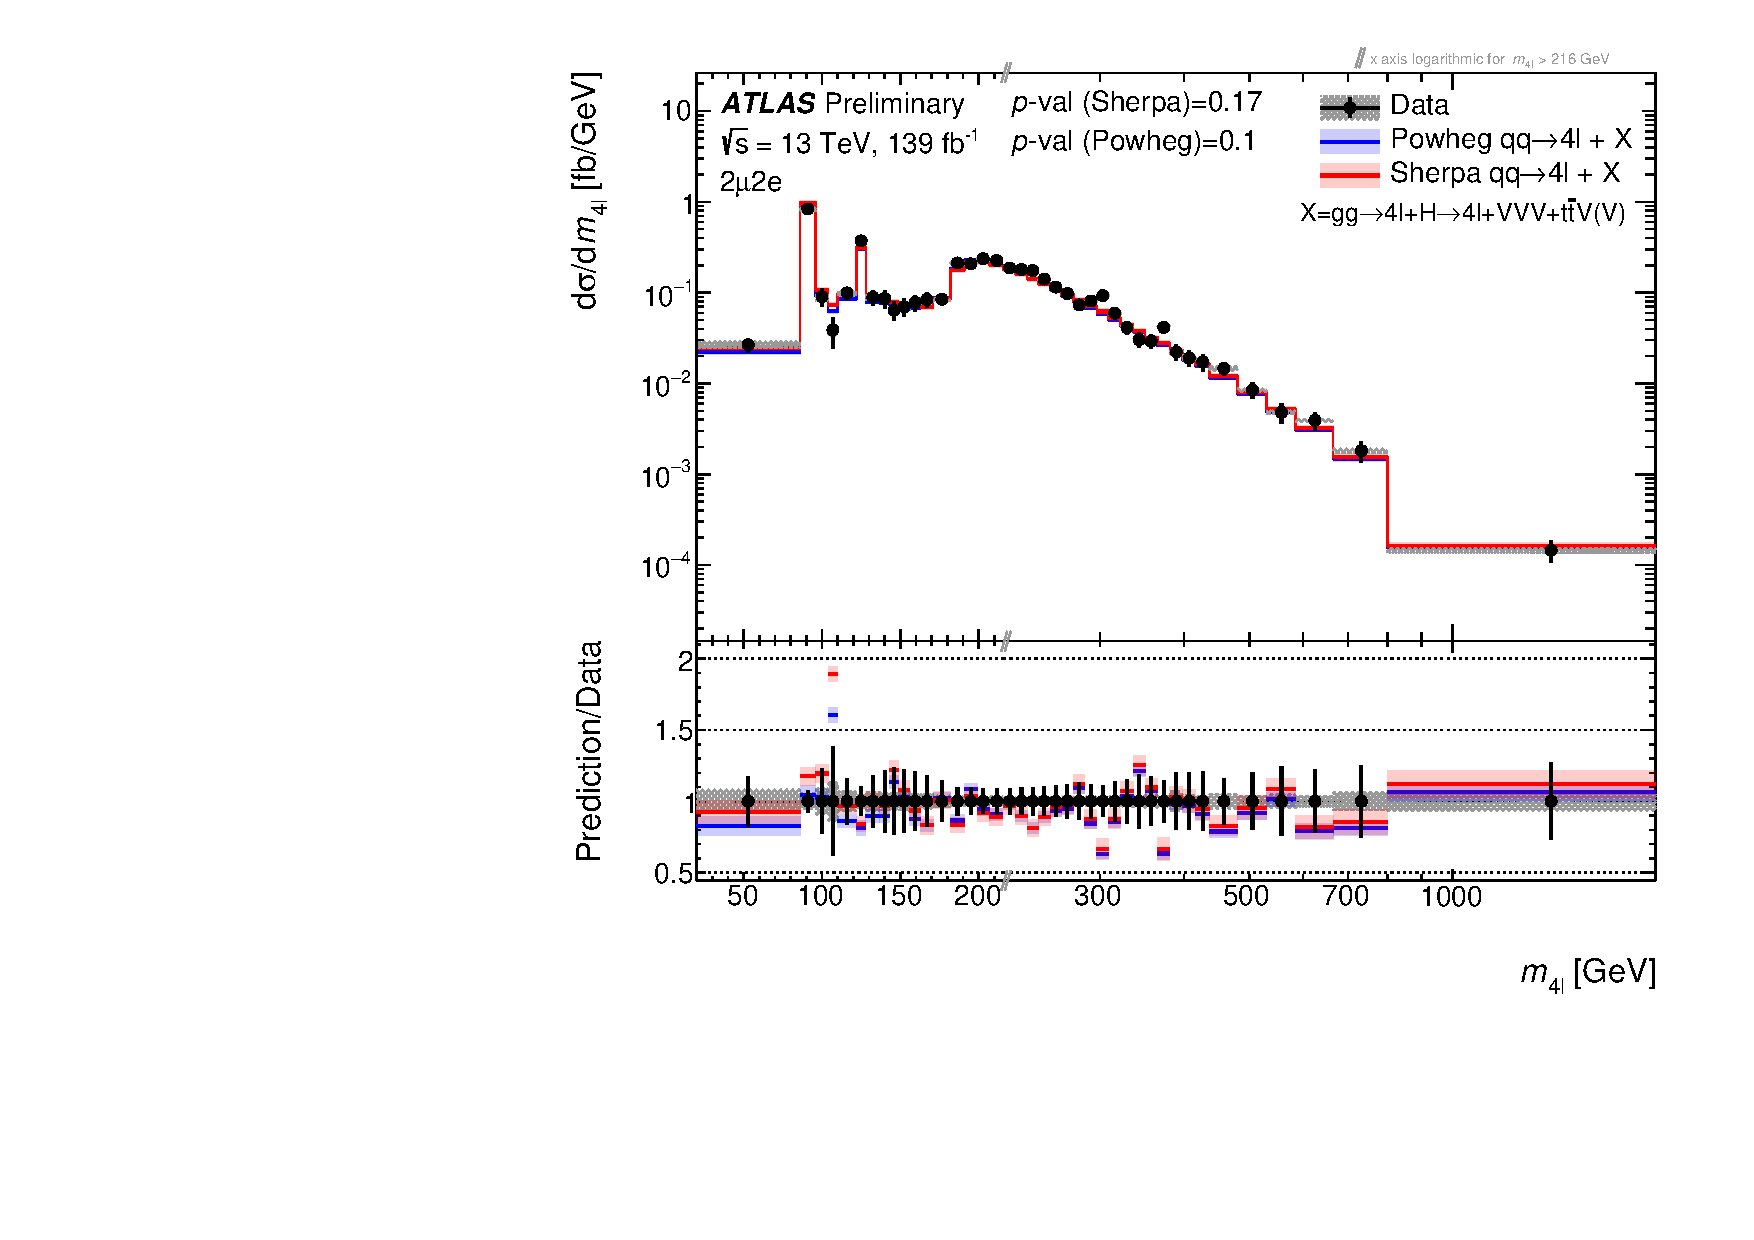
\includegraphics[width=.99\linewidth]{Figures/m4l/UnfoldedResults/linlog_Unfolded_Data_m4l_event_type2mu2e.pdf}  \caption{$2e2\mu$ channel}\label{fig:sub-third}
    \end{subfigure}
    \caption{Differential cross-section as a function of \mFourL{} for each lepton flavour channel. The measured data (black points)  are compared with the SM prediction using either \SHERPA{} (red, with red hashed band for the uncertainty) or \POWHEG{} + \pythia{} (blue, with blue hashed band for the uncertainty) to model the \qqFourL{} contribution. The error bars on the data points give the total uncertainty and the grey hashed band gives the systematic uncertainty. \Pvalue{} The lower panel shows the ratio of the SM predictions to the data.  The $x$-axis is on a linear scale until $\mFourL = 225$~\GeV, where it switches to a logarithmic scale.}
    \label{fig:m4l_flavour}
\end{figure}

%% m12 vs m4l
\begin{figure}[htb!]
    \begin{subfigure}{.49\textwidth}\centering
      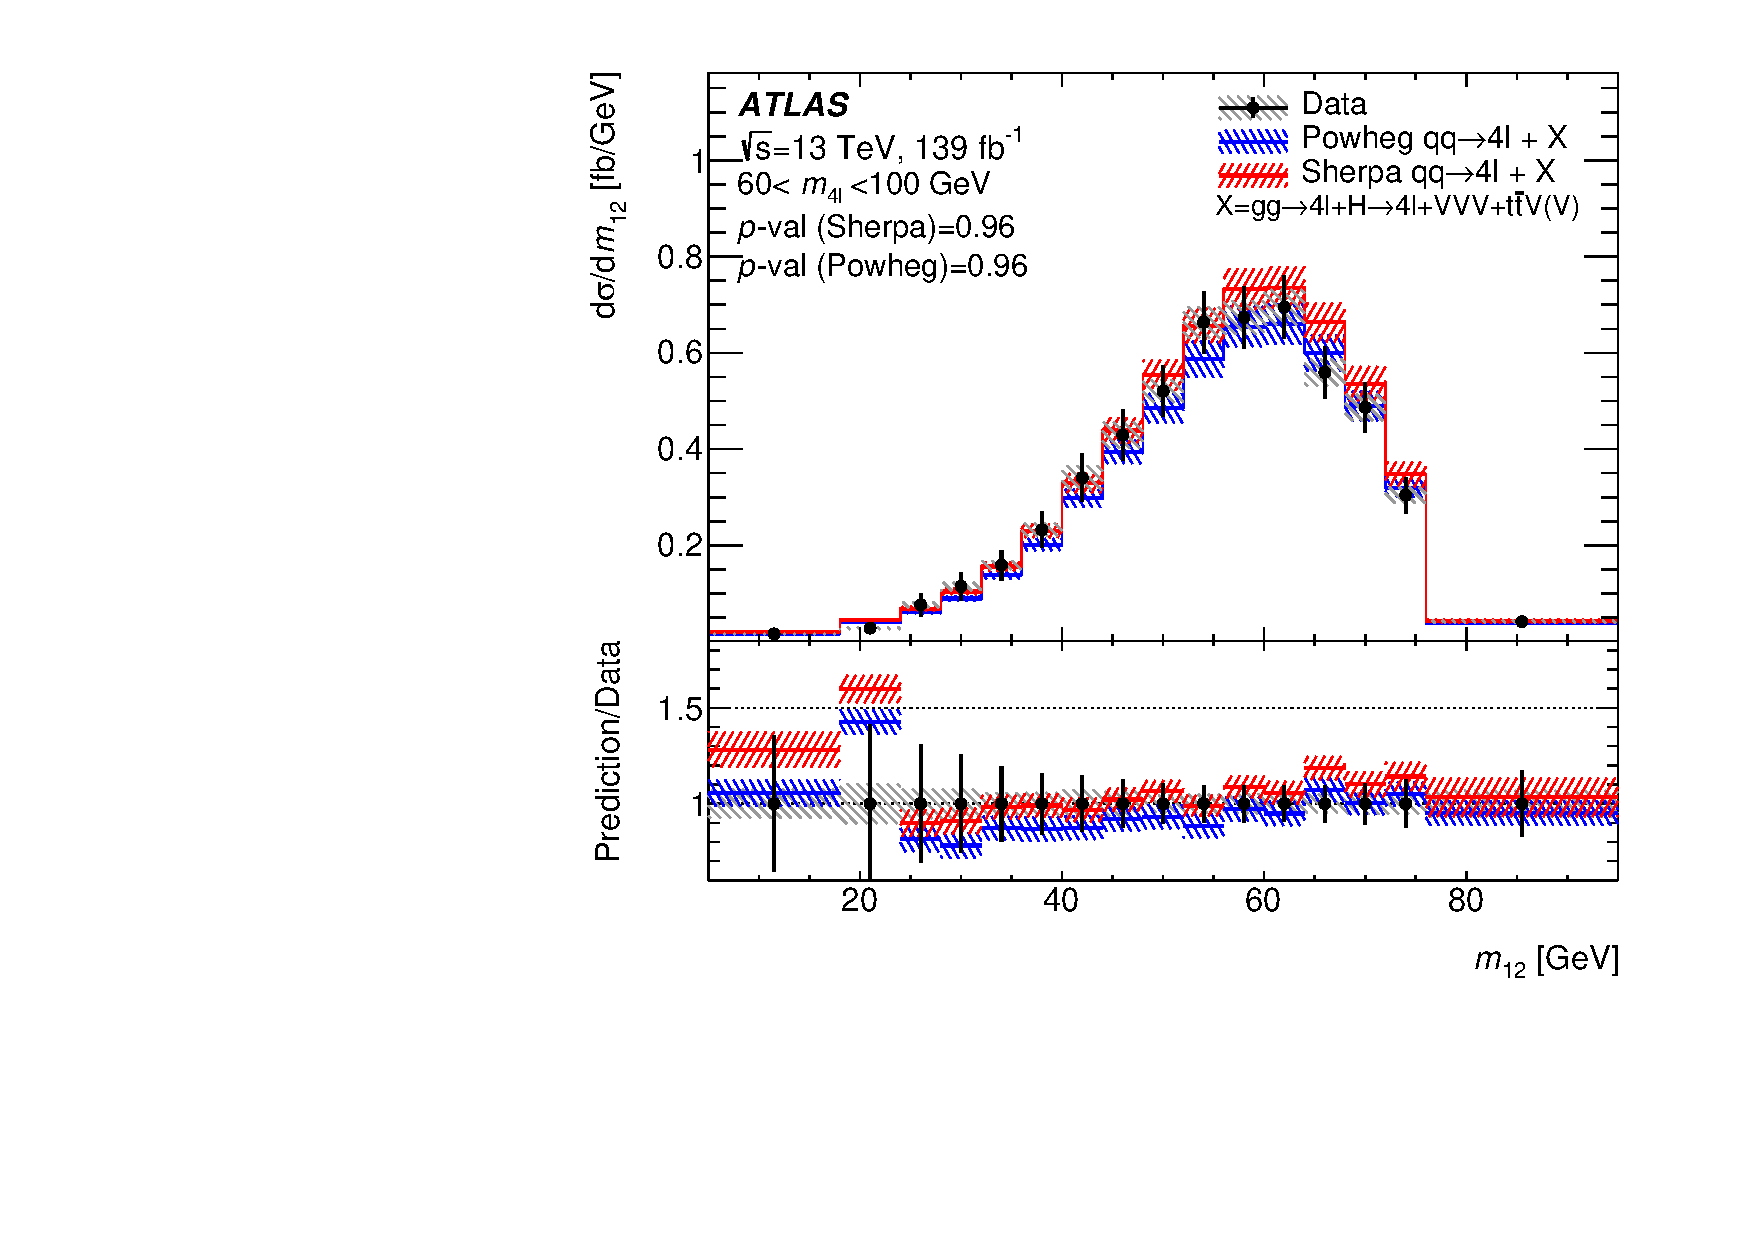
\includegraphics[width=.99\linewidth]{Figures/m4l/UnfoldedResults/linY_Unfolded_Data_m12_m4l60-100.pdf}  
      \caption{\ZFourL \ region}
      \label{fig:sub-first}
    \end{subfigure}
    \begin{subfigure}{.49\textwidth}\centering
      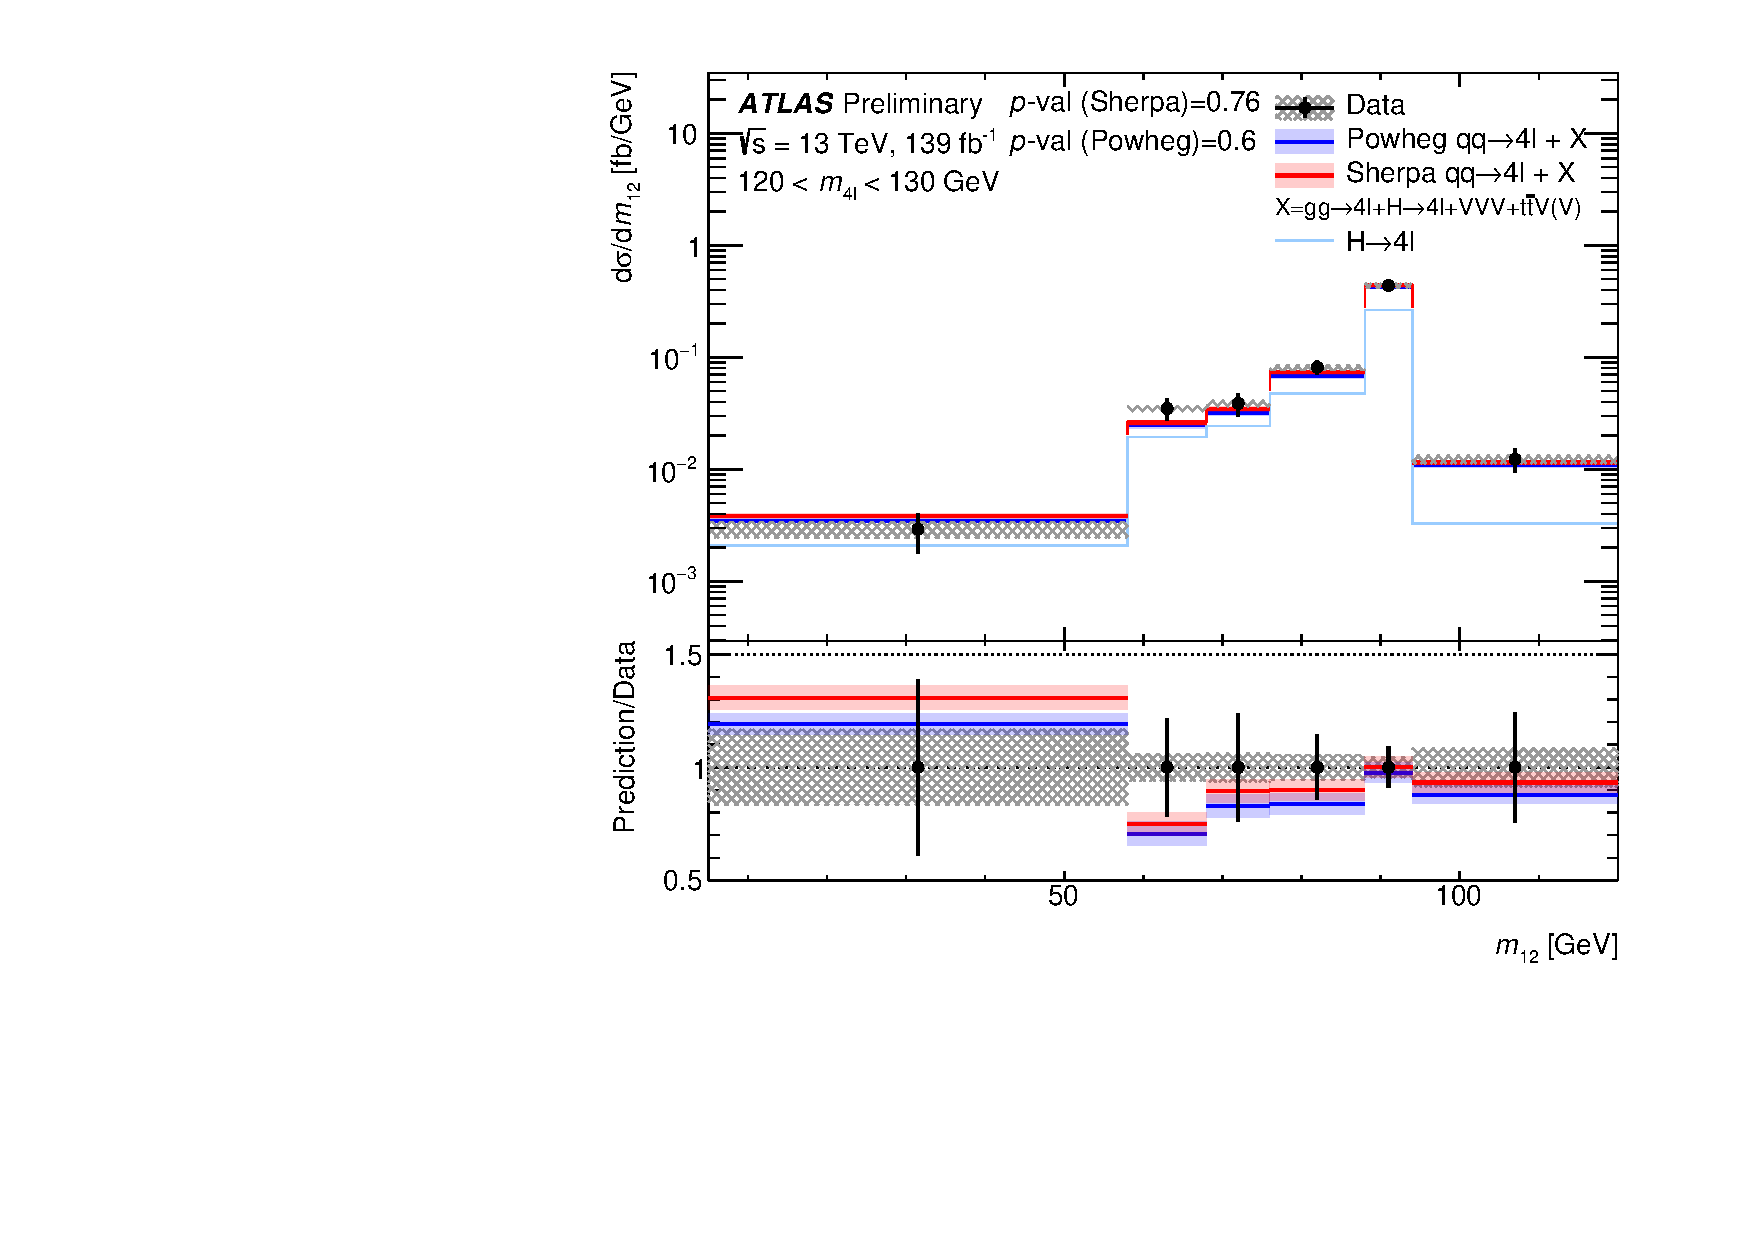
\includegraphics[width=.99\linewidth]{Figures/m4l/UnfoldedResults/higgs_Unfolded_Data_m12_m4l120-130.pdf}  
      \caption{\HFourL \ region}
      \label{fig:sub-second}
    \end{subfigure}
    \begin{subfigure}{.49\textwidth}
      \centering
      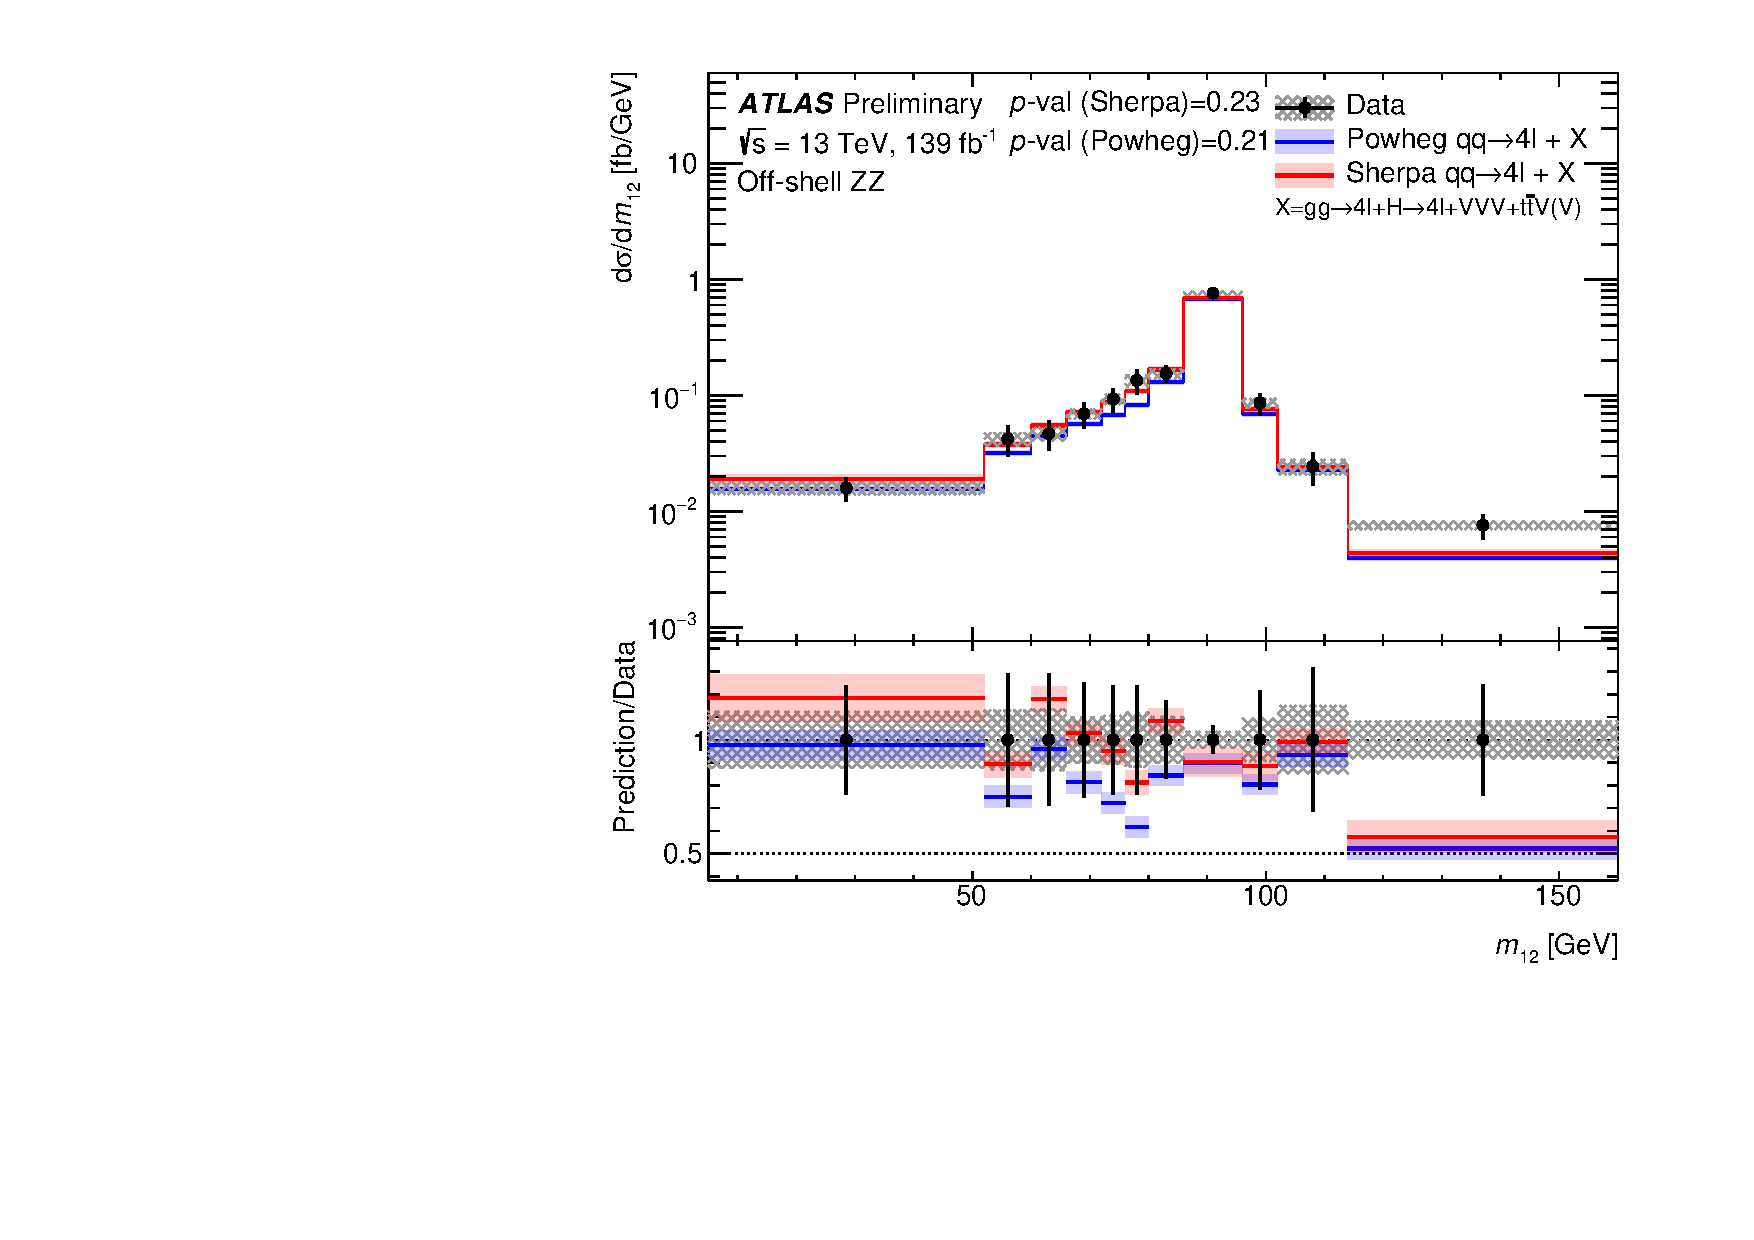
\includegraphics[width=.99\linewidth]{Figures/m4l/UnfoldedResults/Unfolded_Data_m12_m4loffshell.pdf}  
      \caption{Off-shell $\Z\Z$ region}
      \label{fig:sub-third}
    \end{subfigure}
    \begin{subfigure}{.49\textwidth}
      \centering
      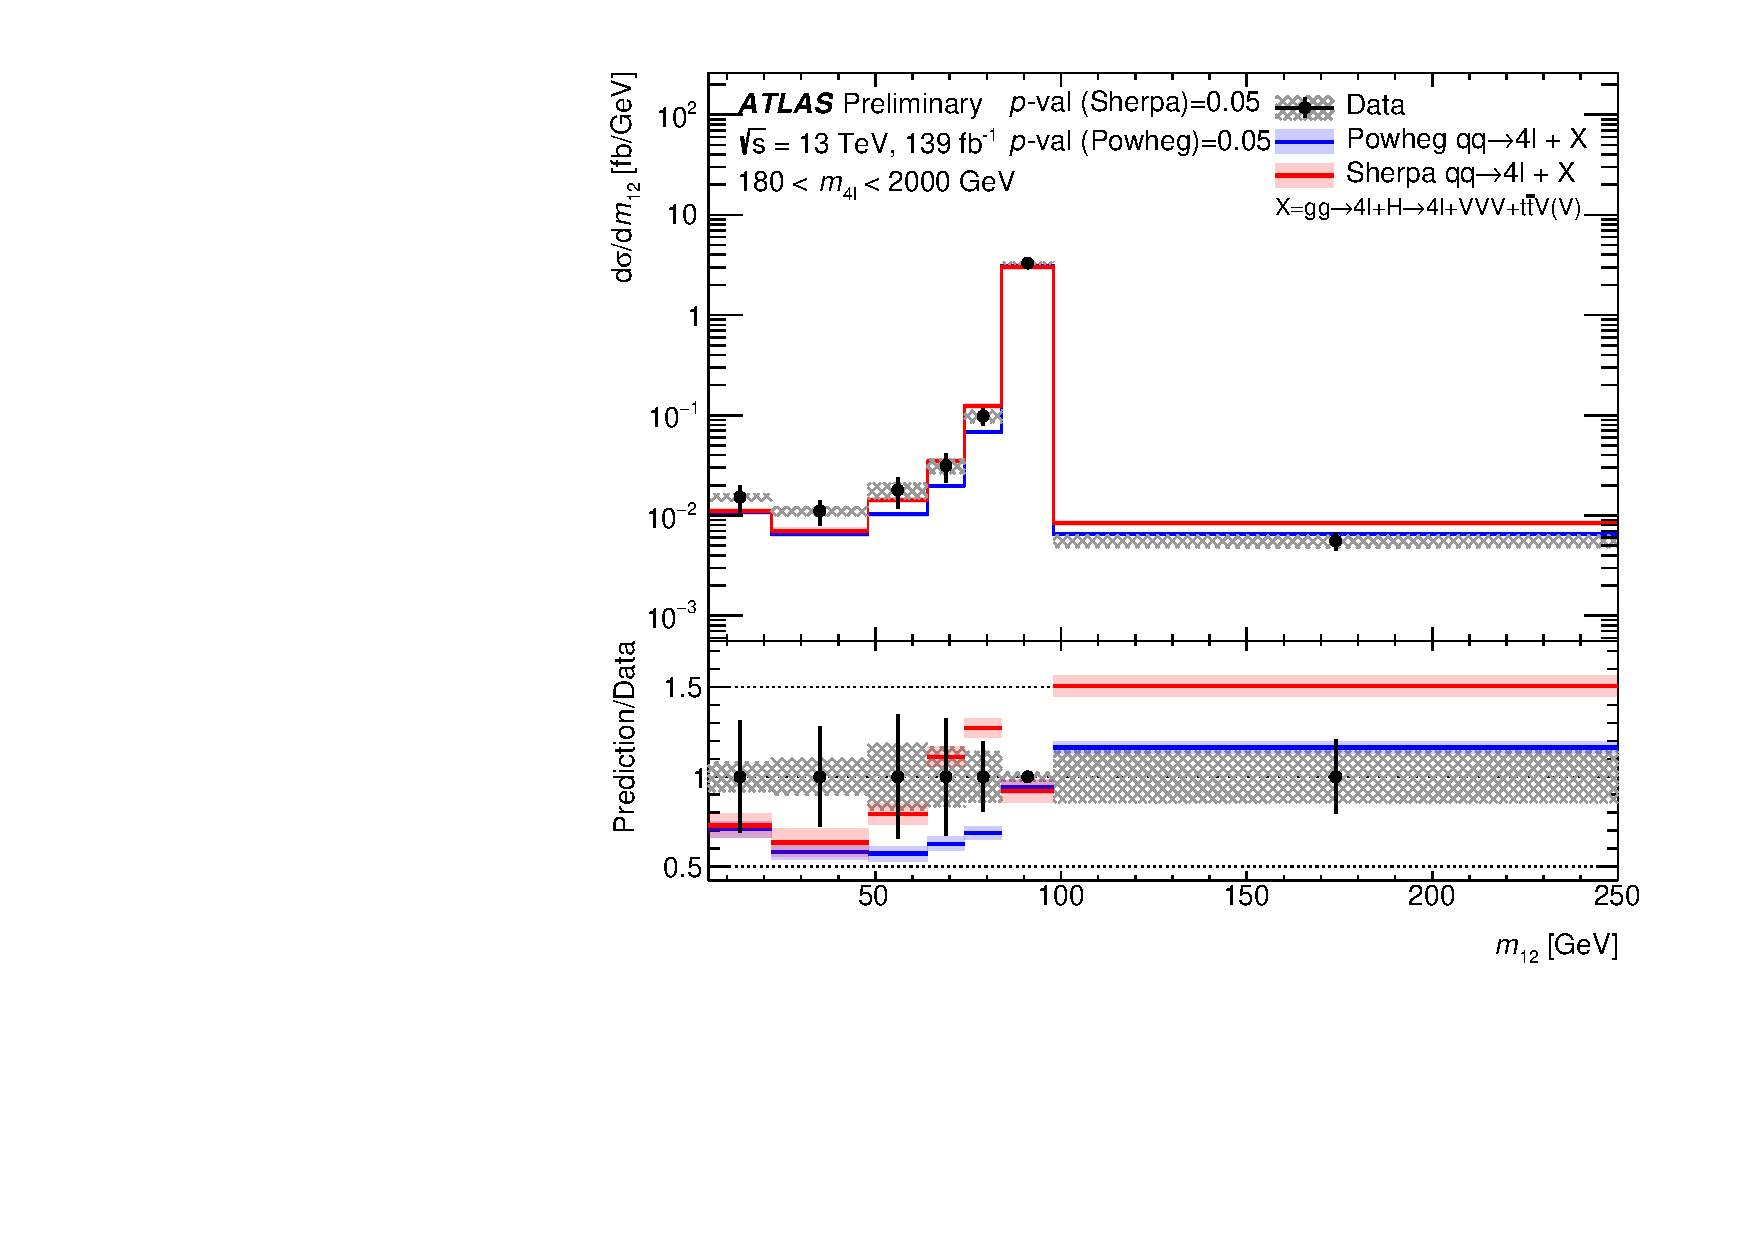
\includegraphics[width=.99\linewidth]{Figures/m4l/UnfoldedResults/Unfolded_Data_m12_m4l180-2000.pdf}  
      \caption{On-shell $\Z\Z$ region}
      \label{fig:sub-fourth}
    \end{subfigure}
    \caption{Differential cross-section as a function of \mZOne{} in the four
        \mFourL{} regions. The measured data (black points) are  compared with the SM prediction using either \SHERPA{} (red, with red hashed band for the uncertainty) or \POWHEG{} + \pythia{} (blue, with blue hashed band for the uncertainty) to model the \qqFourL{} contribution. In (b) the contribution from Higgs production is shown in addition to the total SM prediction. The error bars on the data points give the total uncertainty and the grey hashed band gives the systematic uncertainty. \Pvalue{} The  lower panel shows the ratio of the SM predictions to the data.}
    \label{fig:m12_m4l}
\end{figure}

%% m34 vs m4l
\begin{figure}[htb!]
    \begin{subfigure}{.49\textwidth}\centering
      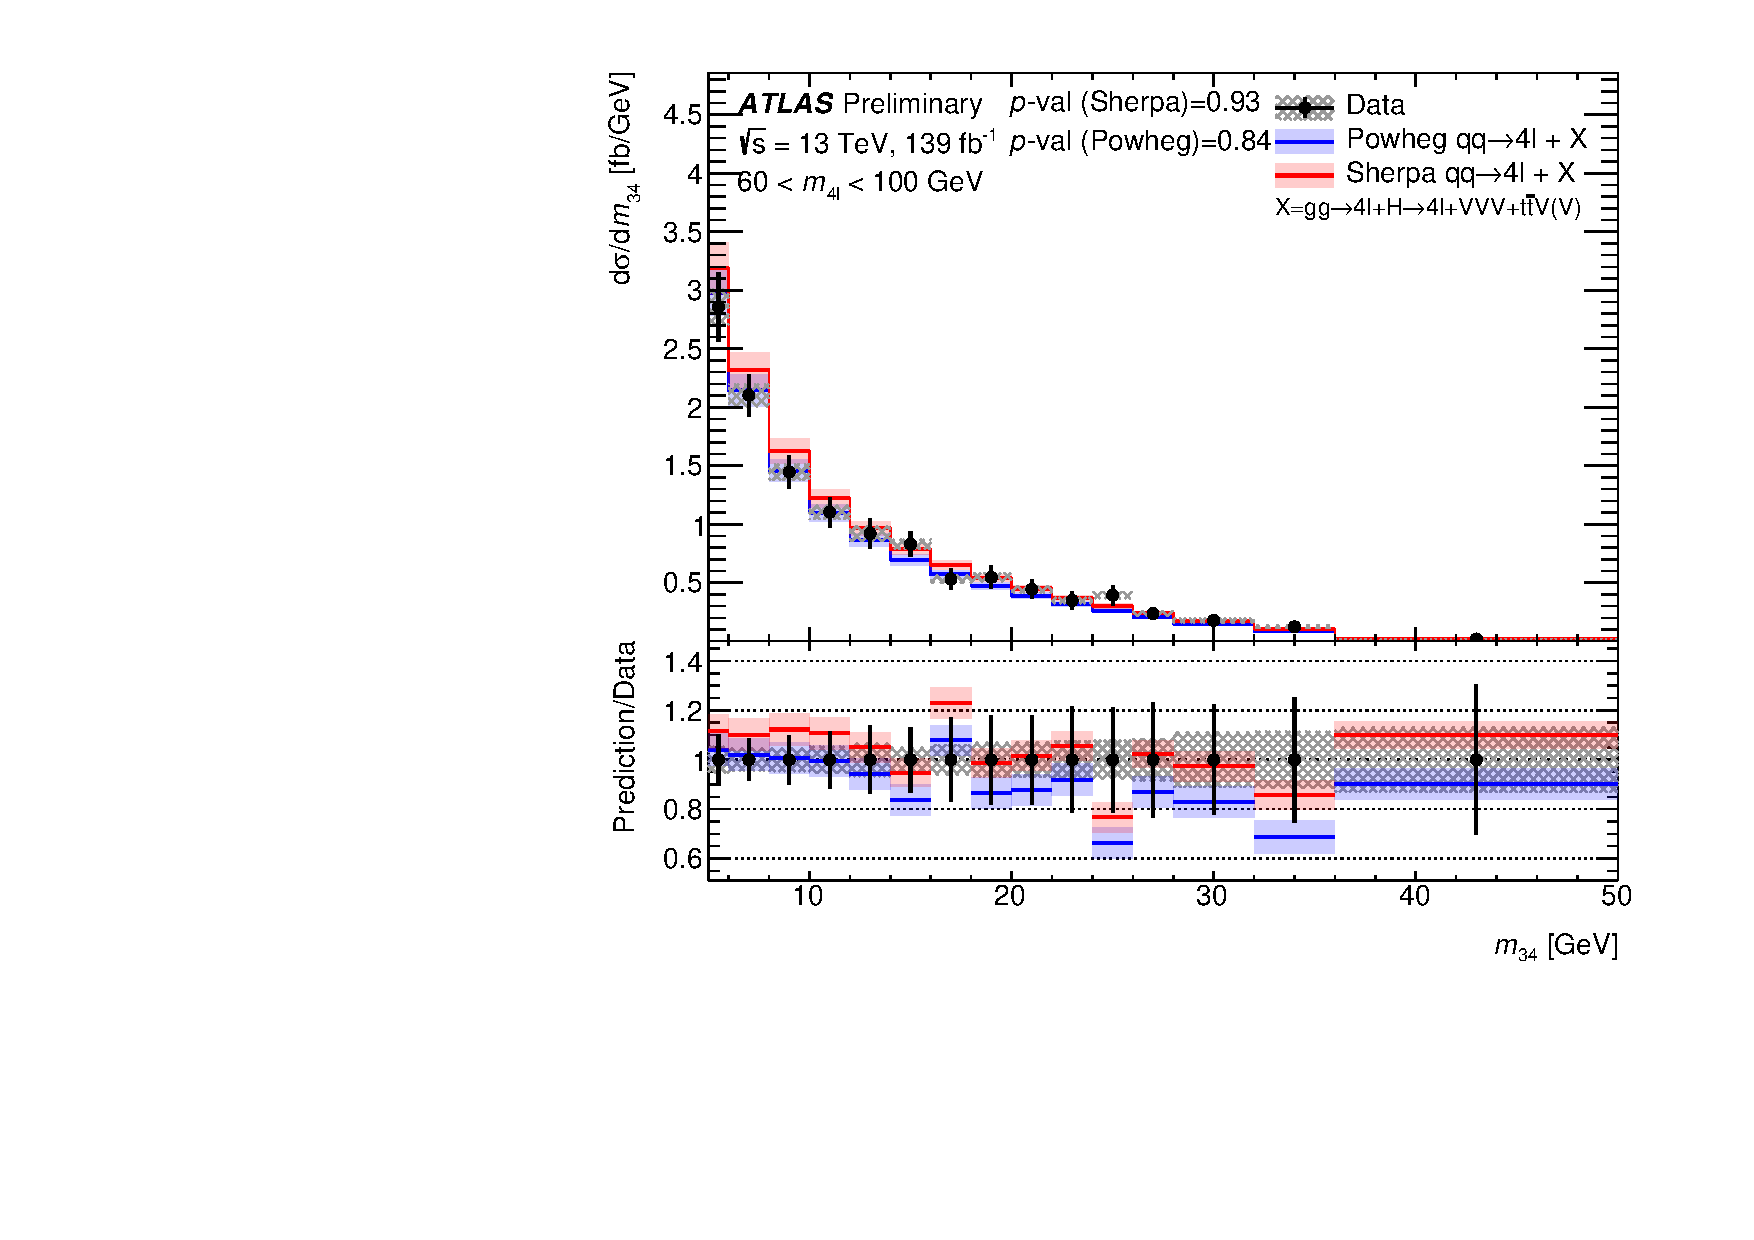
\includegraphics[width=.99\linewidth]{Figures/m4l/UnfoldedResults/linY_Unfolded_Data_m34_m4l60-100.pdf}\caption{\ZFourL \ region}\label{fig:sub-first}
    \end{subfigure}
    \begin{subfigure}{.49\textwidth}\centering
      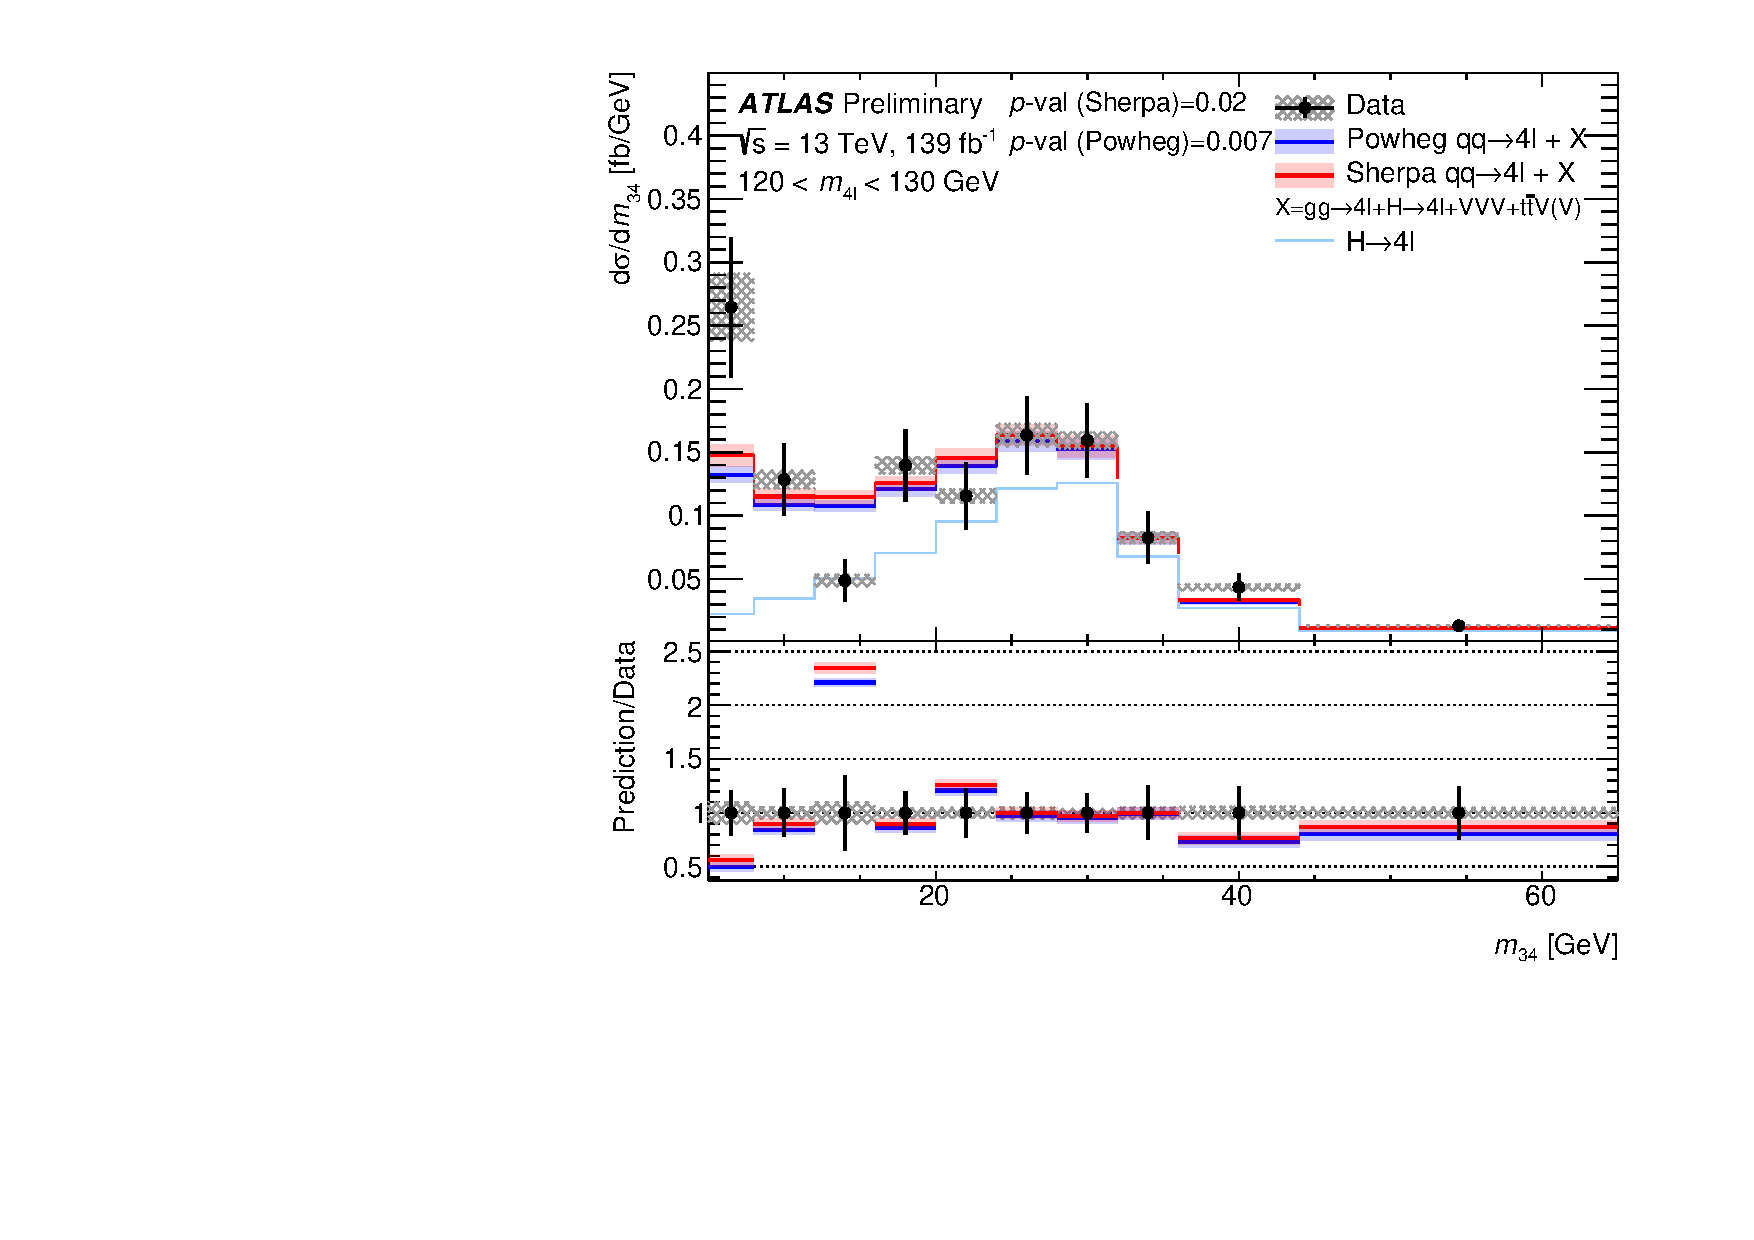
\includegraphics[width=.99\linewidth]{Figures/m4l/UnfoldedResults/higgs_linY_Unfolded_Data_m34_m4l120-130.pdf} \caption{\HFourL \ region}\label{fig:sub-second}
    \end{subfigure}
    \begin{subfigure}{.49\textwidth}\centering
      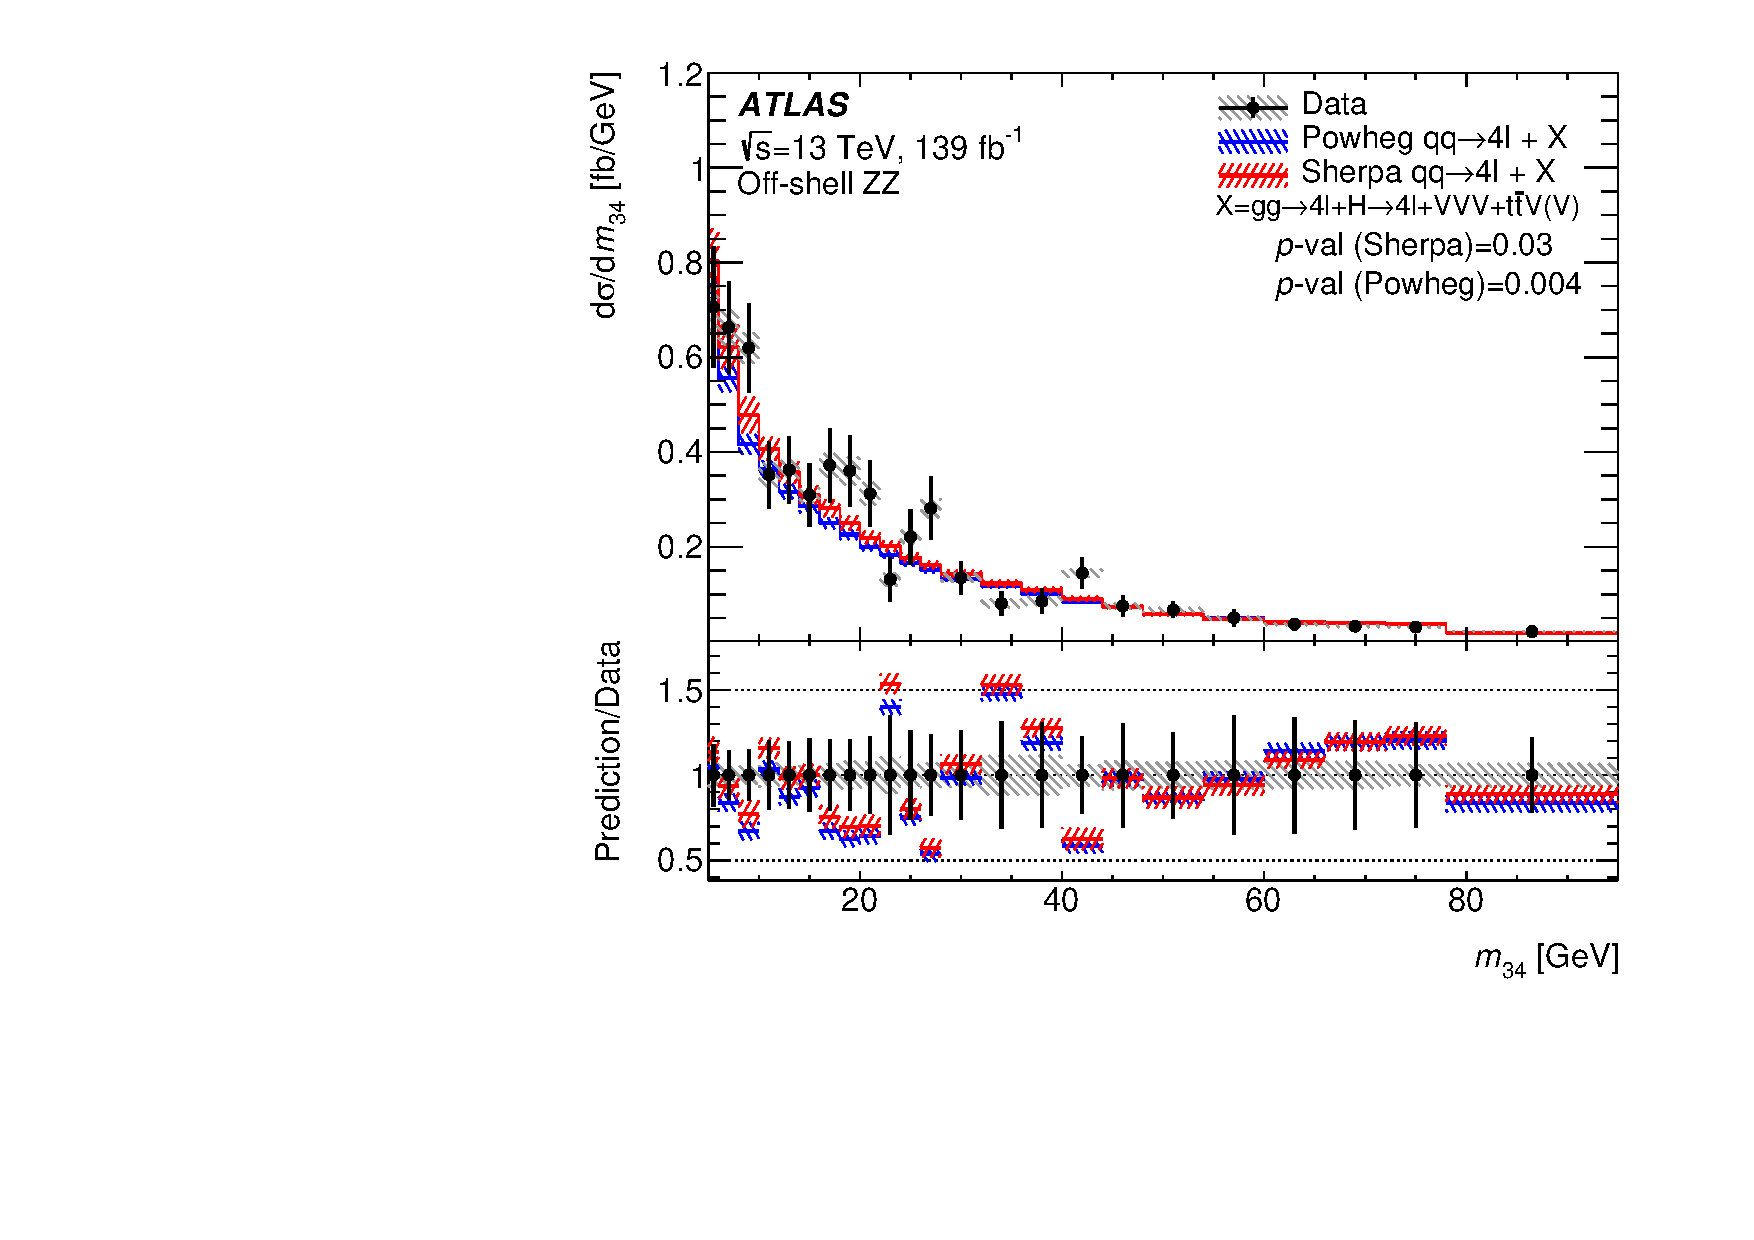
\includegraphics[width=.99\linewidth]{Figures/m4l/UnfoldedResults/linY_Unfolded_Data_m34_m4loffshell.pdf}  \caption{Off-shell $\Z\Z$ region}\label{fig:sub-third}
    \end{subfigure}
    \begin{subfigure}{.49\textwidth}\centering
      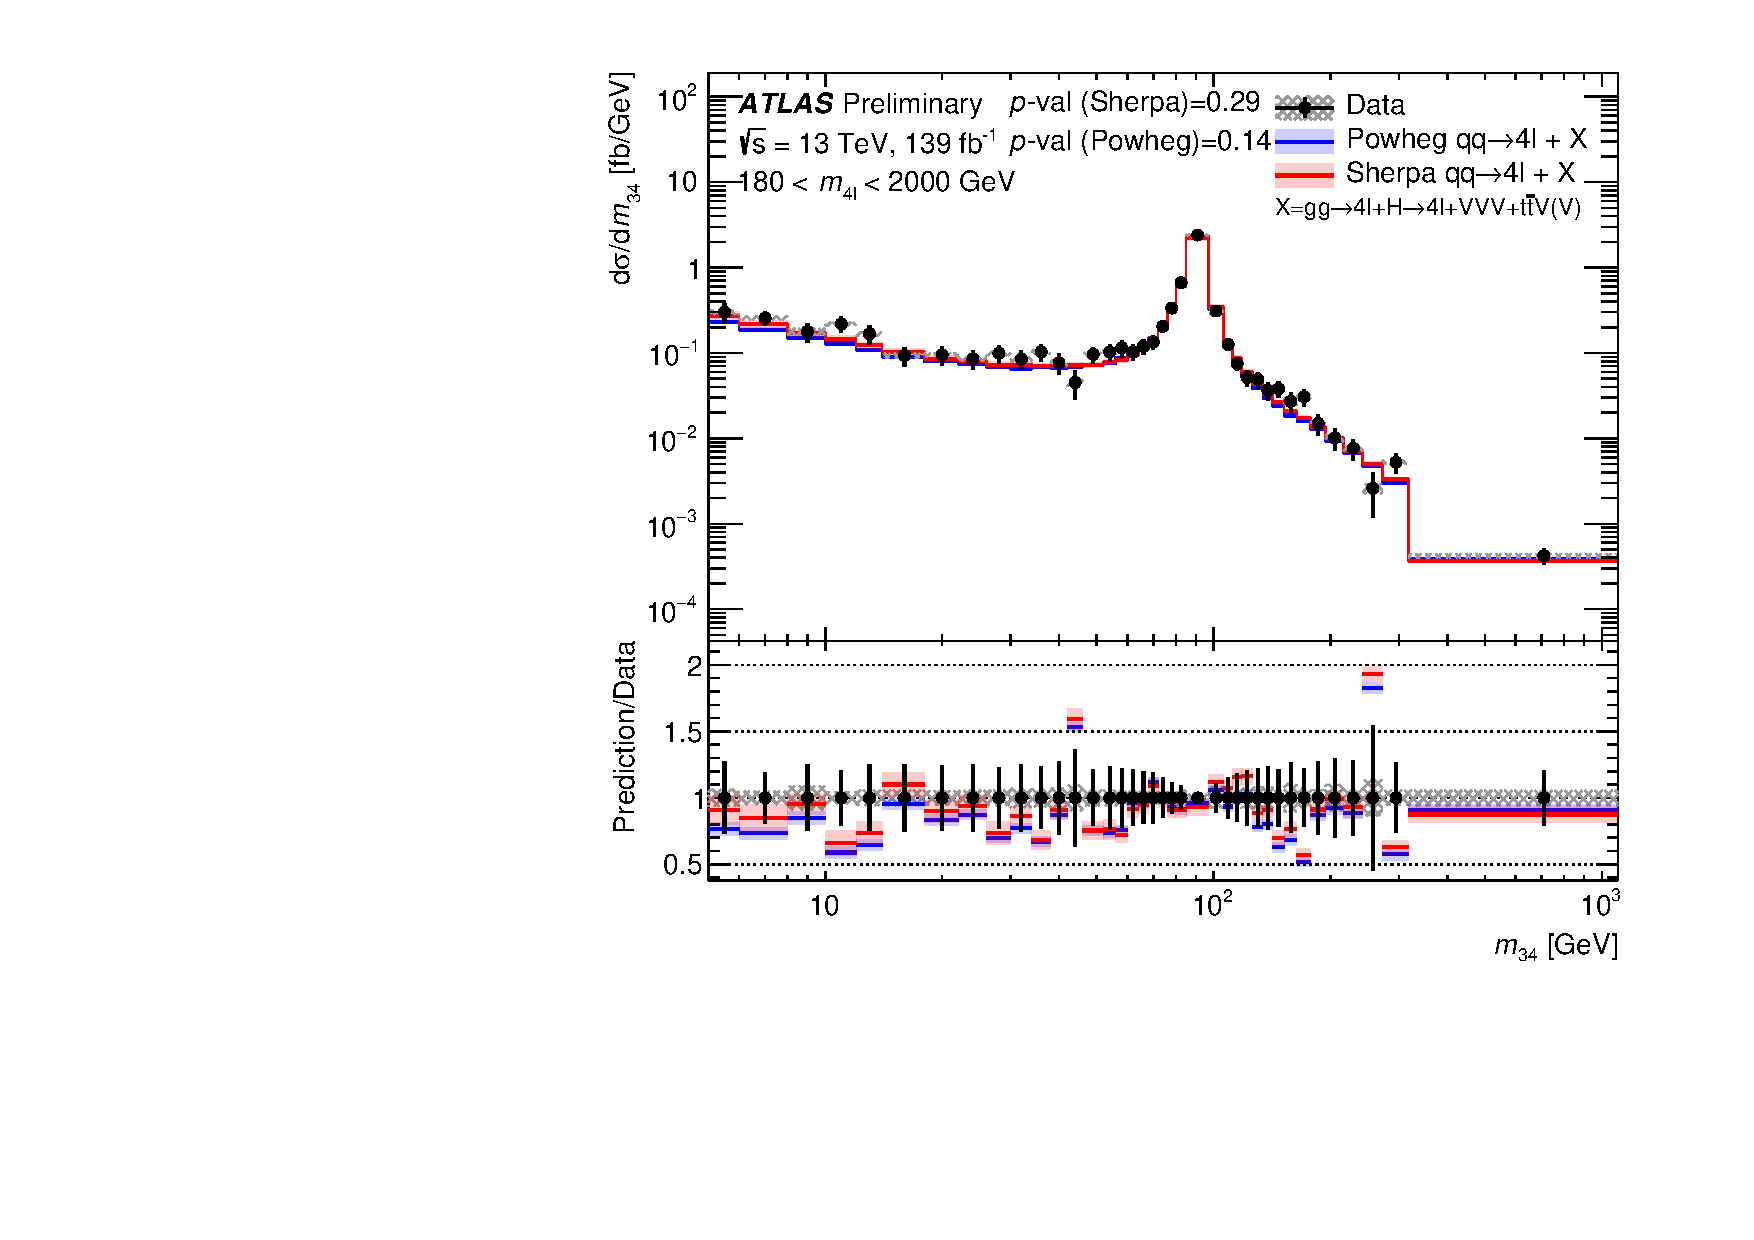
\includegraphics[width=.99\linewidth]{Figures/m4l/UnfoldedResults/Unfolded_Data_m34_m4l180-2000.pdf}  \caption{On-shell $\Z\Z$ region}\label{fig:sub-fourth}
    \end{subfigure}
    \caption{Differential cross-section as a function of \mZTwo{} in the four
        \mFourL{} regions. The measured data (black points) are  compared with the SM prediction using either \SHERPA{} (red, with red hashed band for the uncertainty) or \POWHEG{} + \pythia{} (blue, with blue hashed band for the uncertainty) to model the \qqFourL{} contribution. In (b) the contribution from Higgs production is shown in addition to the total SM prediction. The error bars on the data points give the total uncertainty and the grey hashed band gives the systematic uncertainty. \Pvalue{} The  lower panel shows the ratio of the SM predictions to the data.}
    \label{fig:m34_m4l}
\end{figure}

%% pt12 vs m4l
\begin{figure}[htb!]
    \begin{subfigure}{.49\textwidth}\centering
      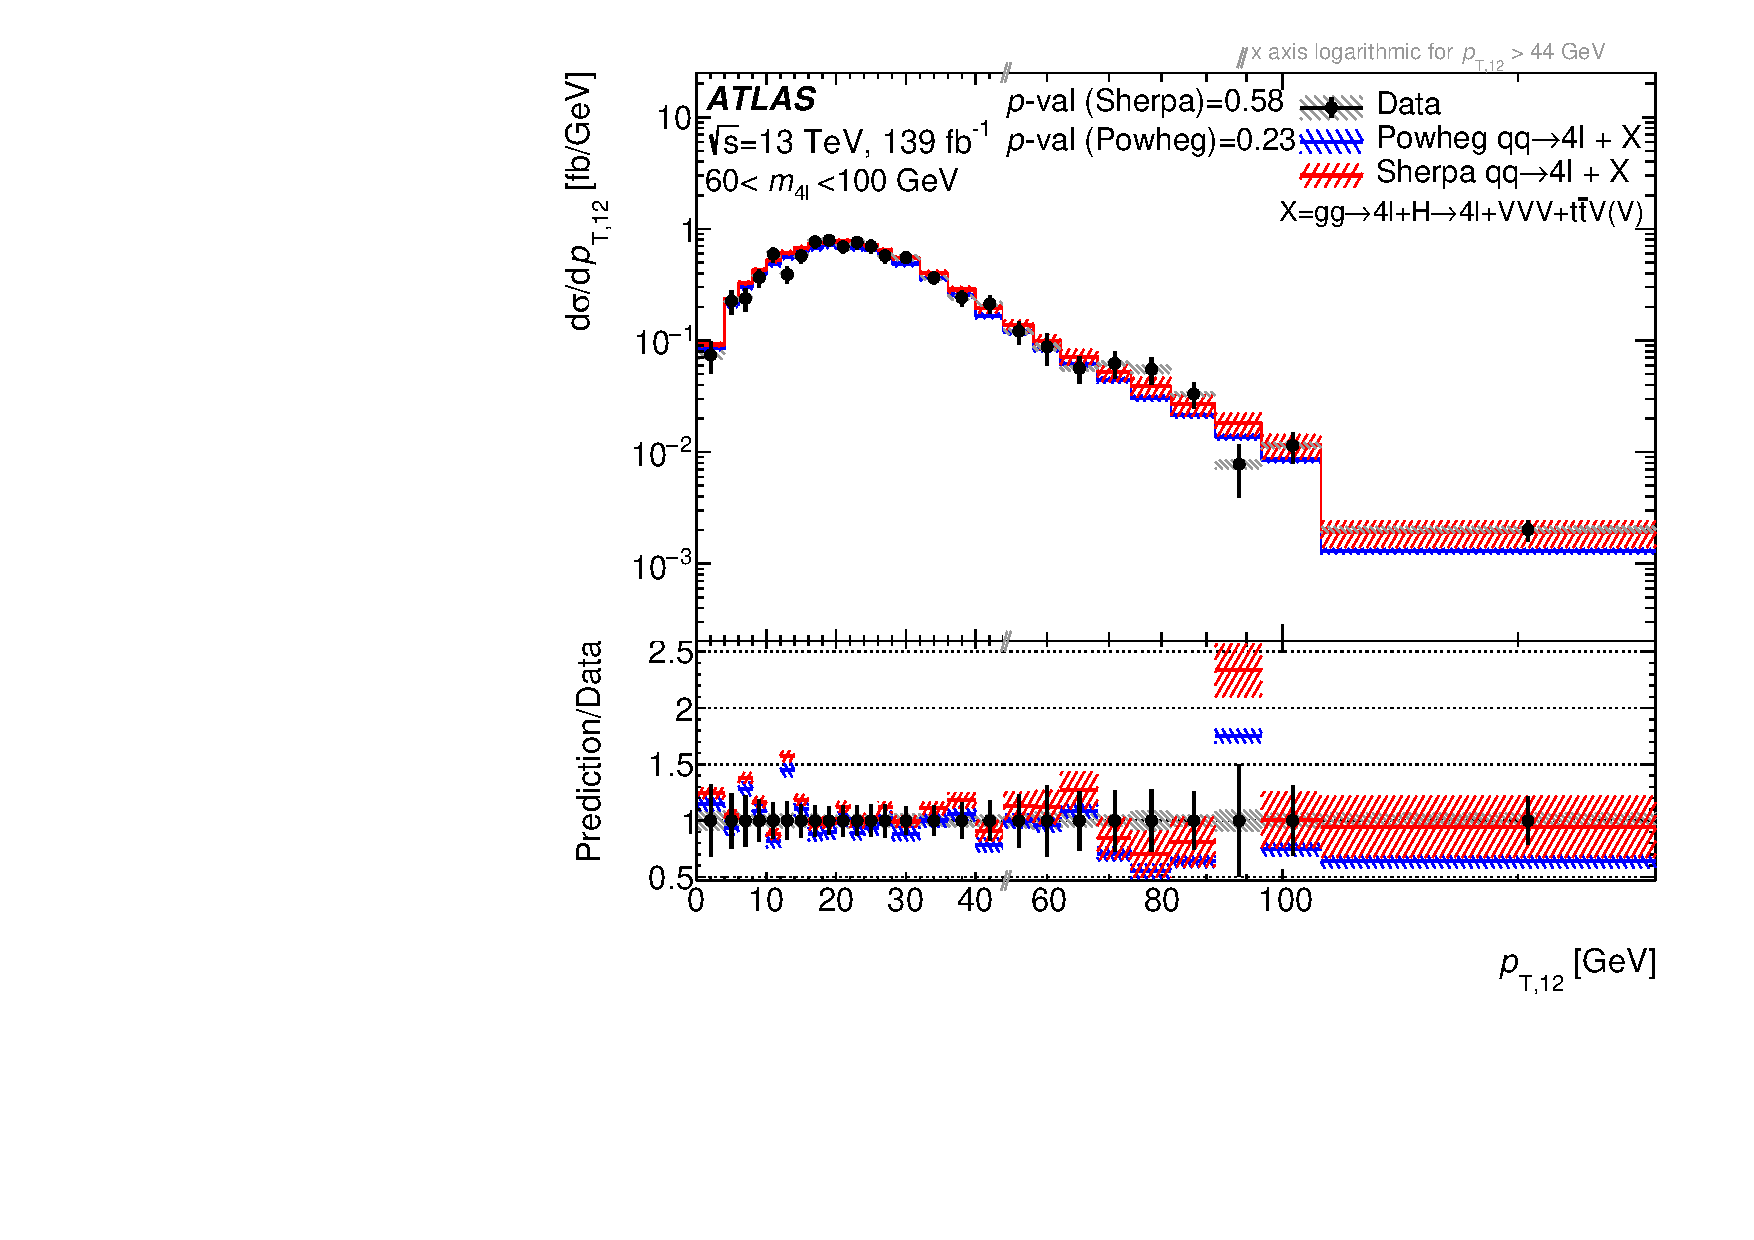
\includegraphics[width=.99\linewidth]{Figures/m4l/UnfoldedResults/linlog_Unfolded_Data_pt12_m4l60-100.pdf}\caption{\ZFourL \ region}\label{fig:sub-first}
    \end{subfigure}
    \begin{subfigure}{.49\textwidth}\centering
      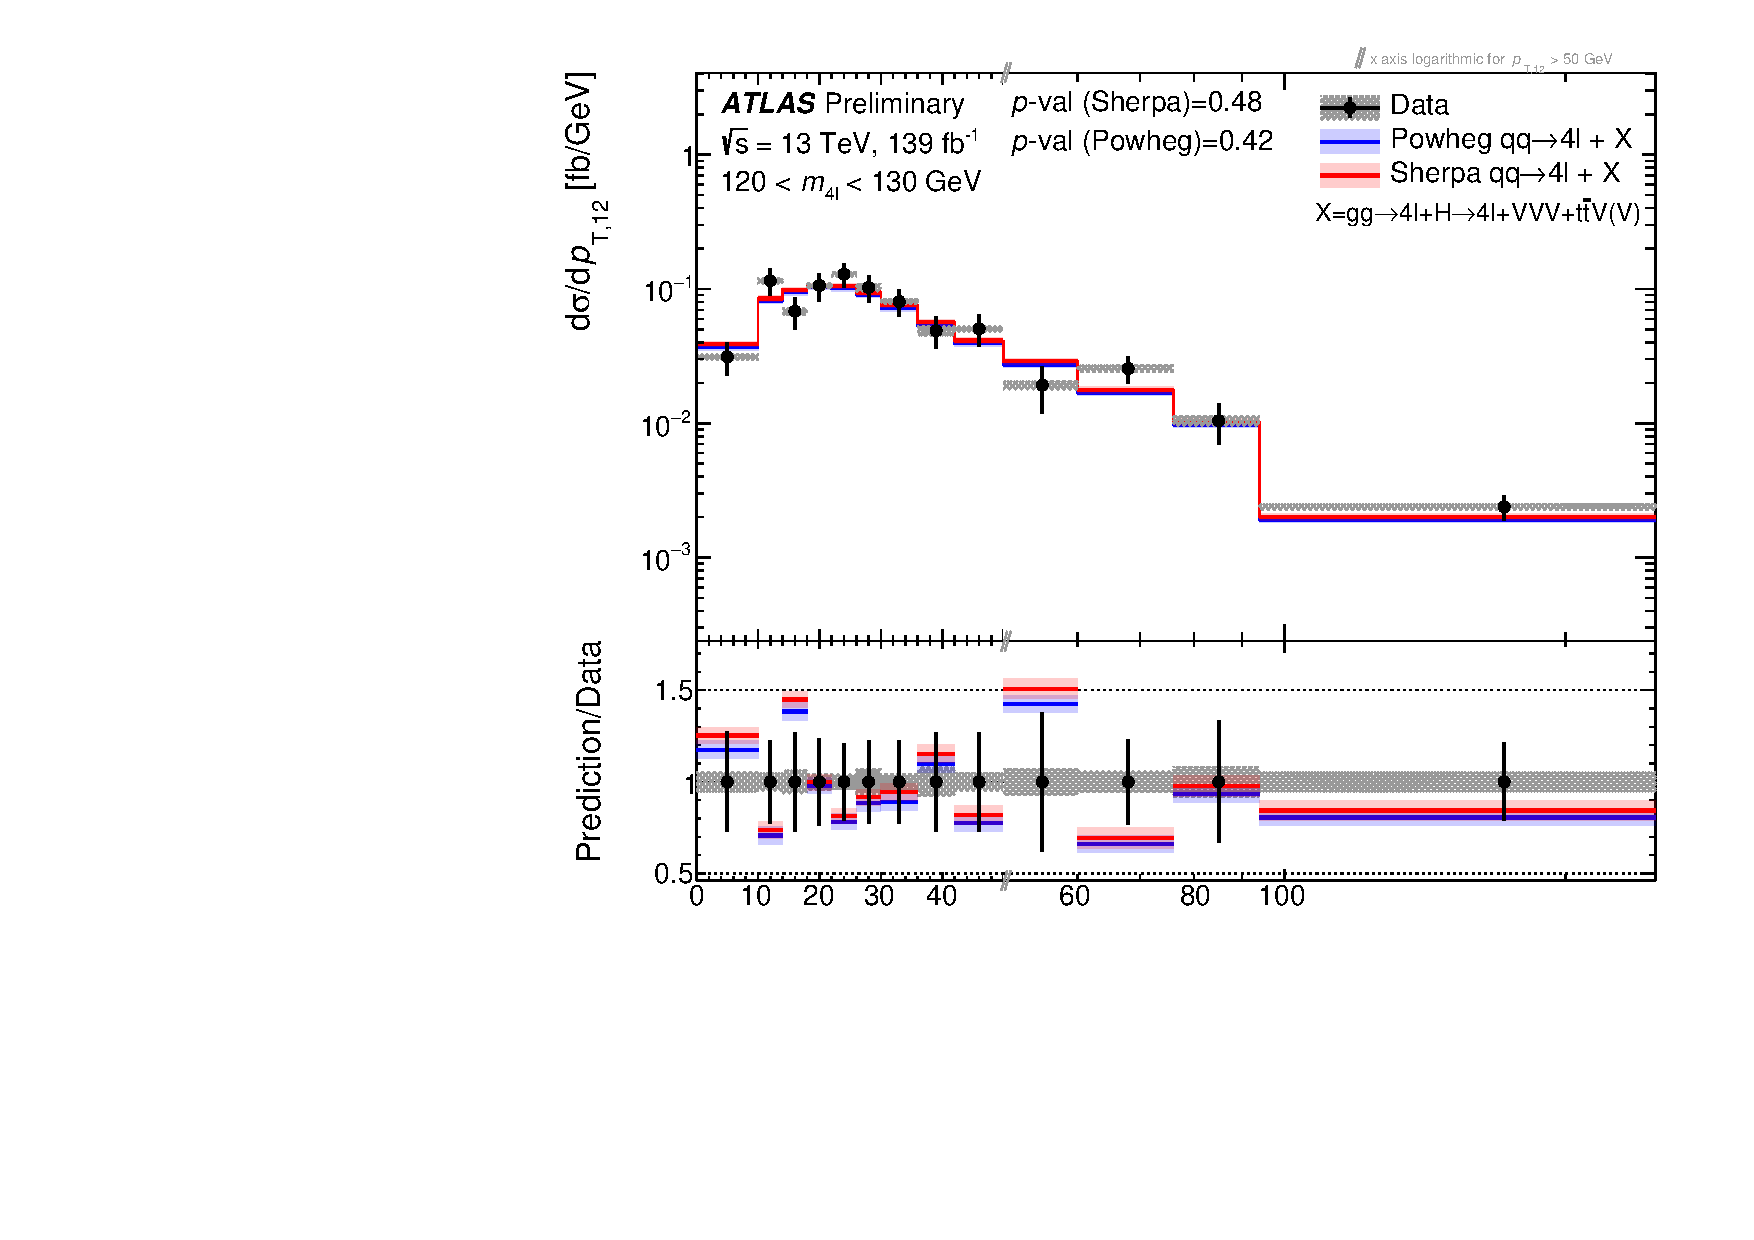
\includegraphics[width=.99\linewidth]{Figures/m4l/UnfoldedResults/linlog_Unfolded_Data_pt12_m4l120-130.pdf} \caption{\HFourL \ region}\label{fig:sub-second}
    \end{subfigure}
    \begin{subfigure}{.49\textwidth}\centering
      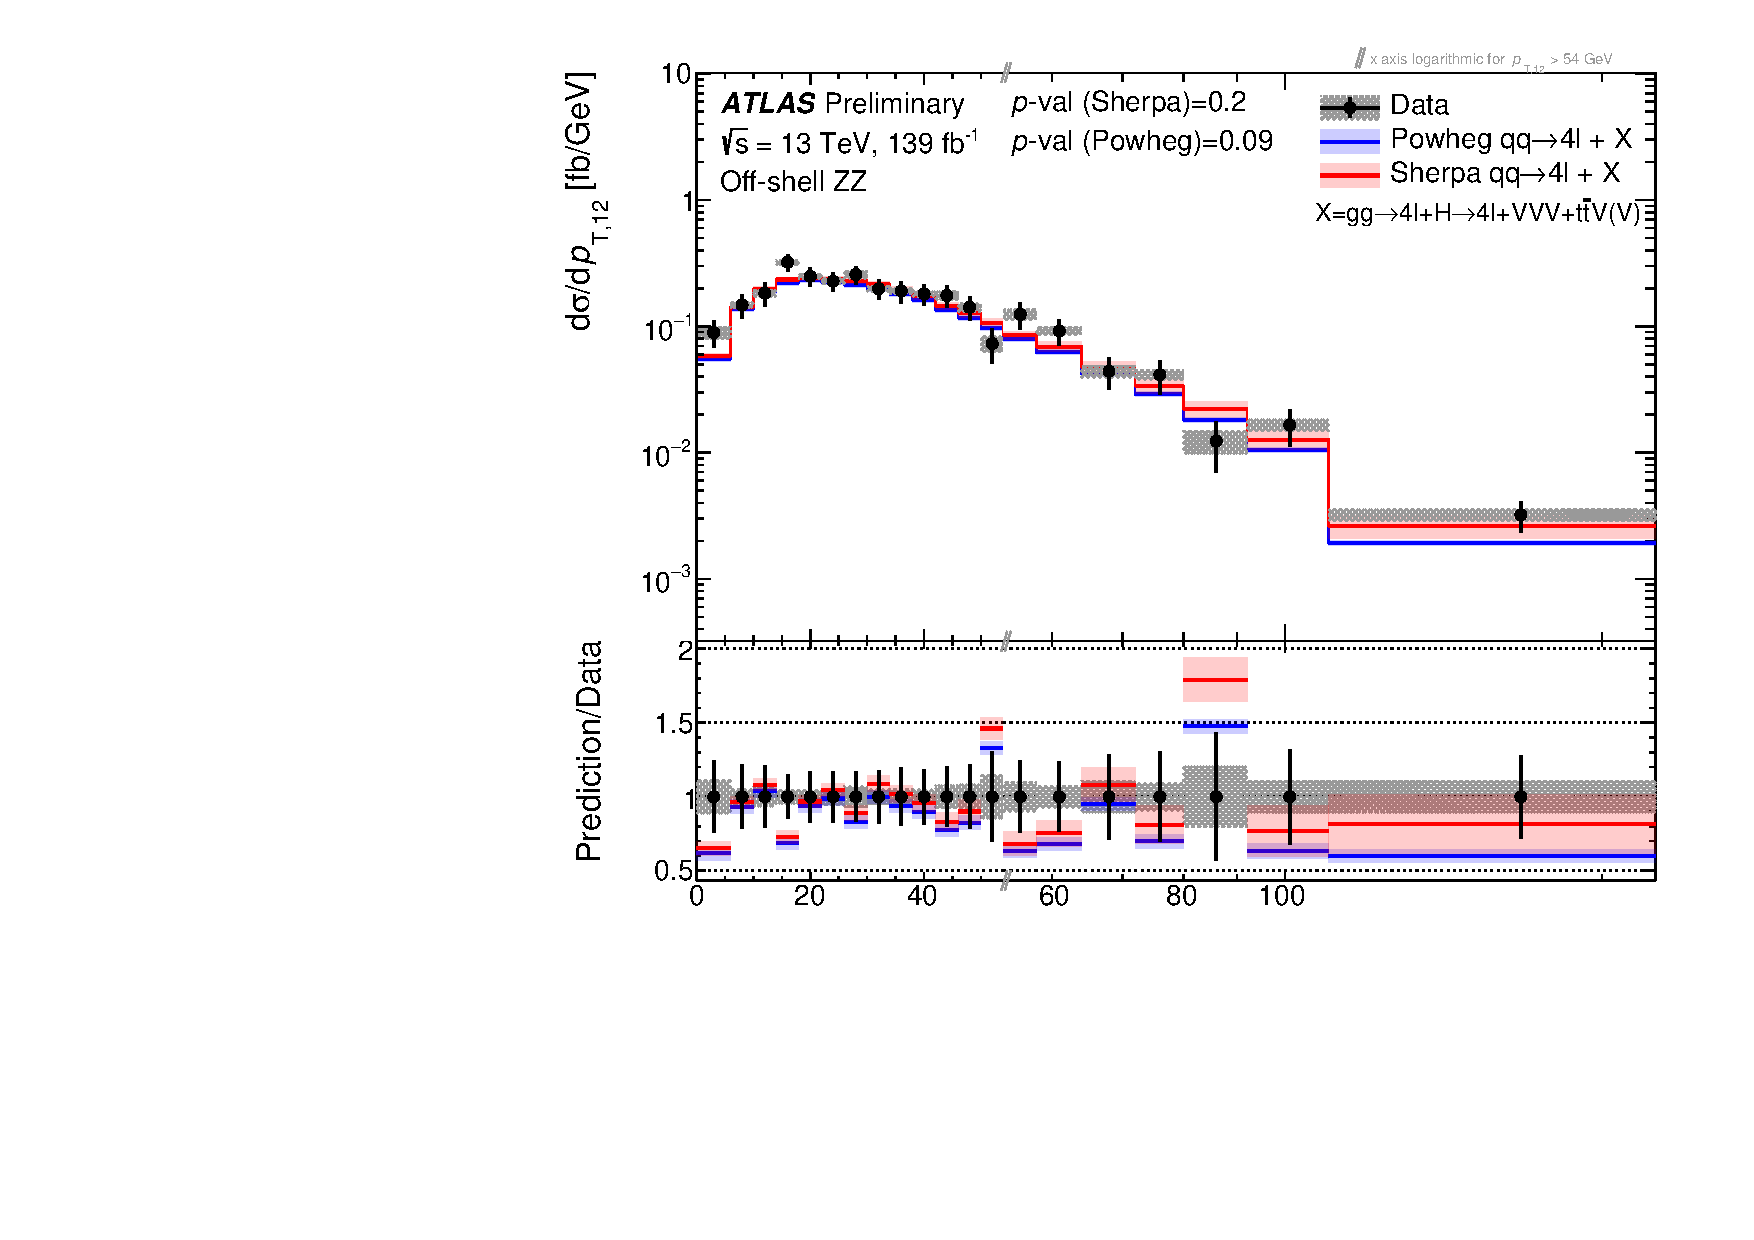
\includegraphics[width=.99\linewidth]{Figures/m4l/UnfoldedResults/linlog_Unfolded_Data_pt12_m4loffshell.pdf}  \caption{Off-shell $\Z\Z$ region}\label{fig:sub-third}
    \end{subfigure}
    \begin{subfigure}{.49\textwidth}\centering
      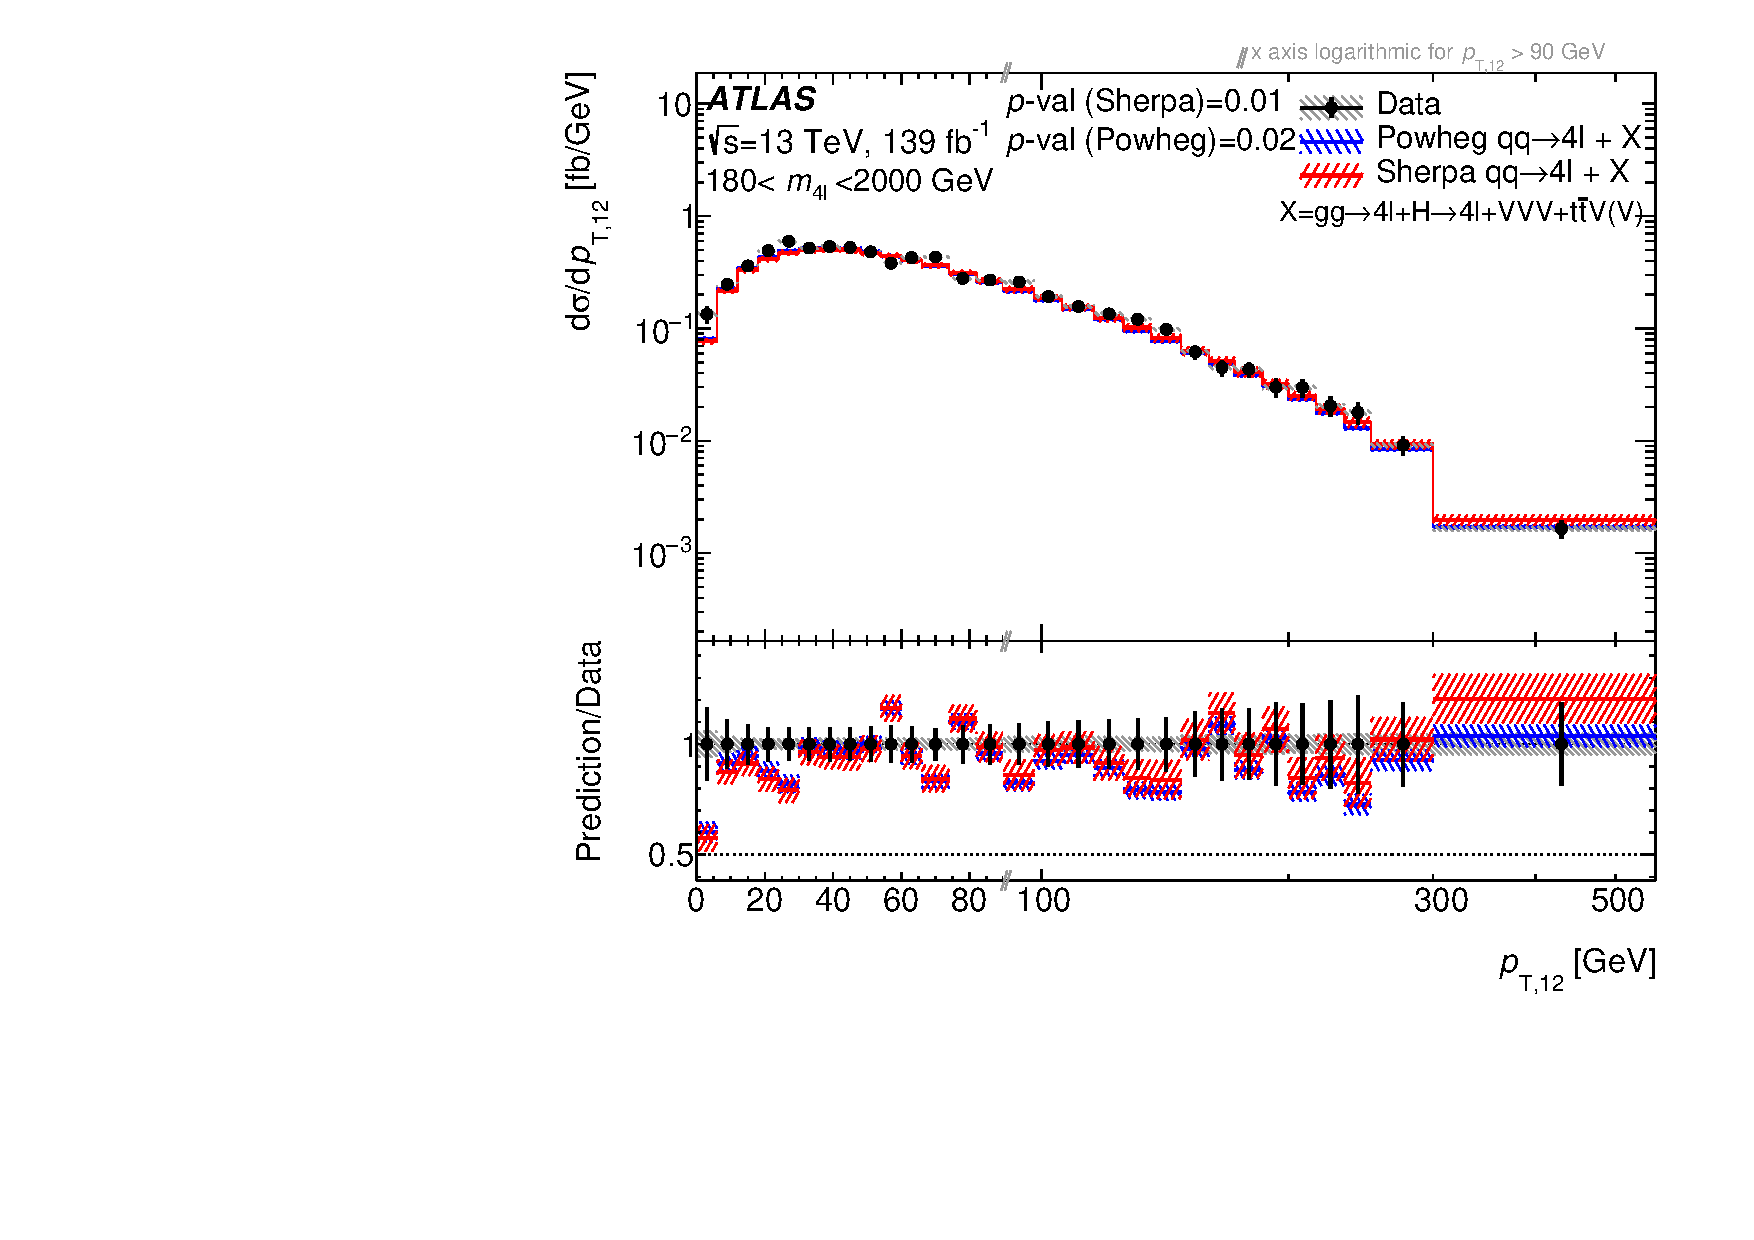
\includegraphics[width=.99\linewidth]{Figures/m4l/UnfoldedResults/linlog_Unfolded_Data_pt12_m4l180-2000.pdf}  \caption{On-shell $\Z\Z$ region}\label{fig:sub-fourth}
    \end{subfigure}
    \caption{Differential cross-section as a function of \ptZOne{} in the four
        \mFourL{} regions. The measured data (black points) are  compared with the SM prediction using either \SHERPA{} (red, with red hashed band for the uncertainty) or \POWHEG{} + \pythia{} (blue, with blue hashed band for the uncertainty) to model the \qqFourL{} contribution. In (b) the contribution from Higgs production is shown in addition to the total SM prediction. The error bars on the data points give the total uncertainty and the grey hashed band gives the systematic uncertainty. \Pvalue{} The  lower panel shows the ratio of the SM predictions to the data.}
    \label{fig:pt12_m4l}
\end{figure}

%% pt34 vs m4l
\begin{figure}[htb!]
    \begin{subfigure}{.49\textwidth}\centering
      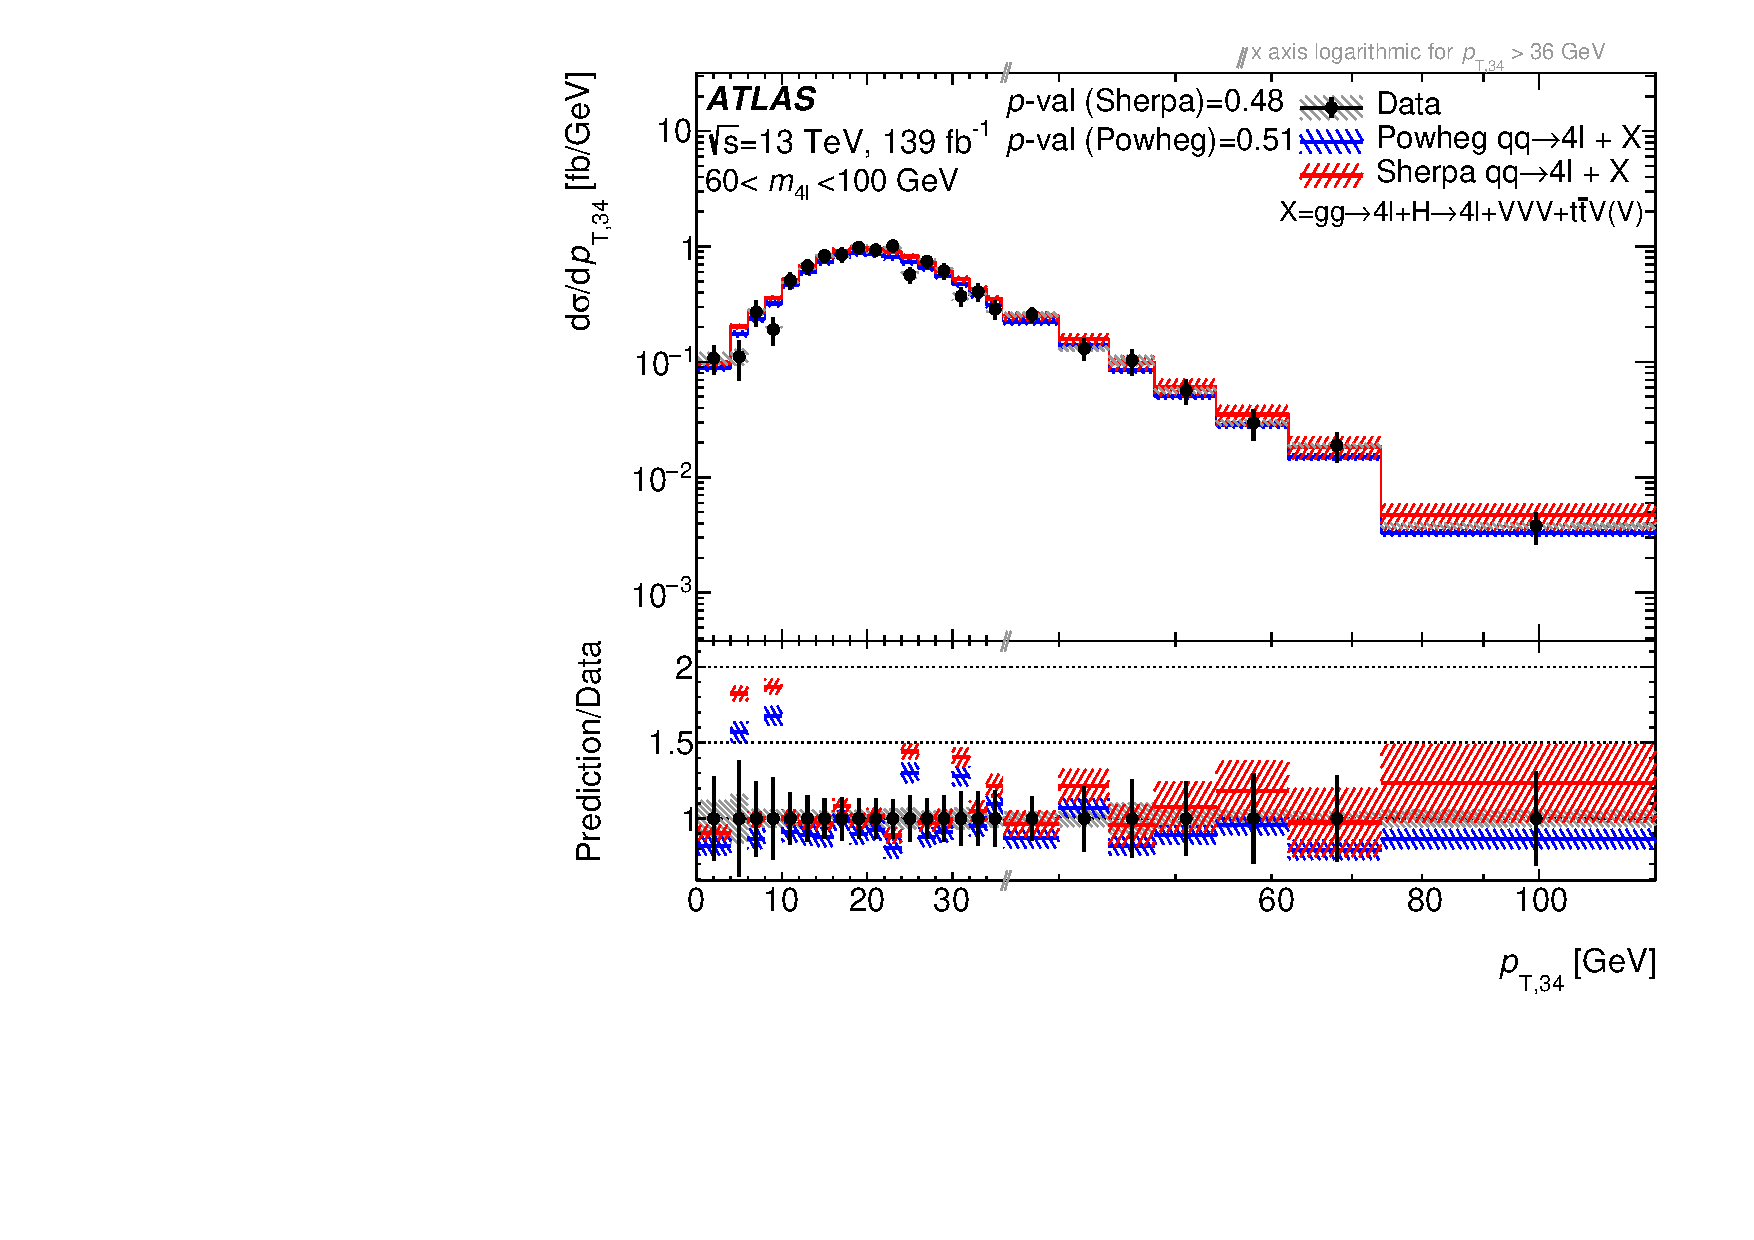
\includegraphics[width=.99\linewidth]{Figures/m4l/UnfoldedResults/linlog_Unfolded_Data_pt34_m4l60-100.pdf}\caption{\ZFourL \ region}\label{fig:sub-first}
    \end{subfigure}
    \begin{subfigure}{.49\textwidth}\centering
      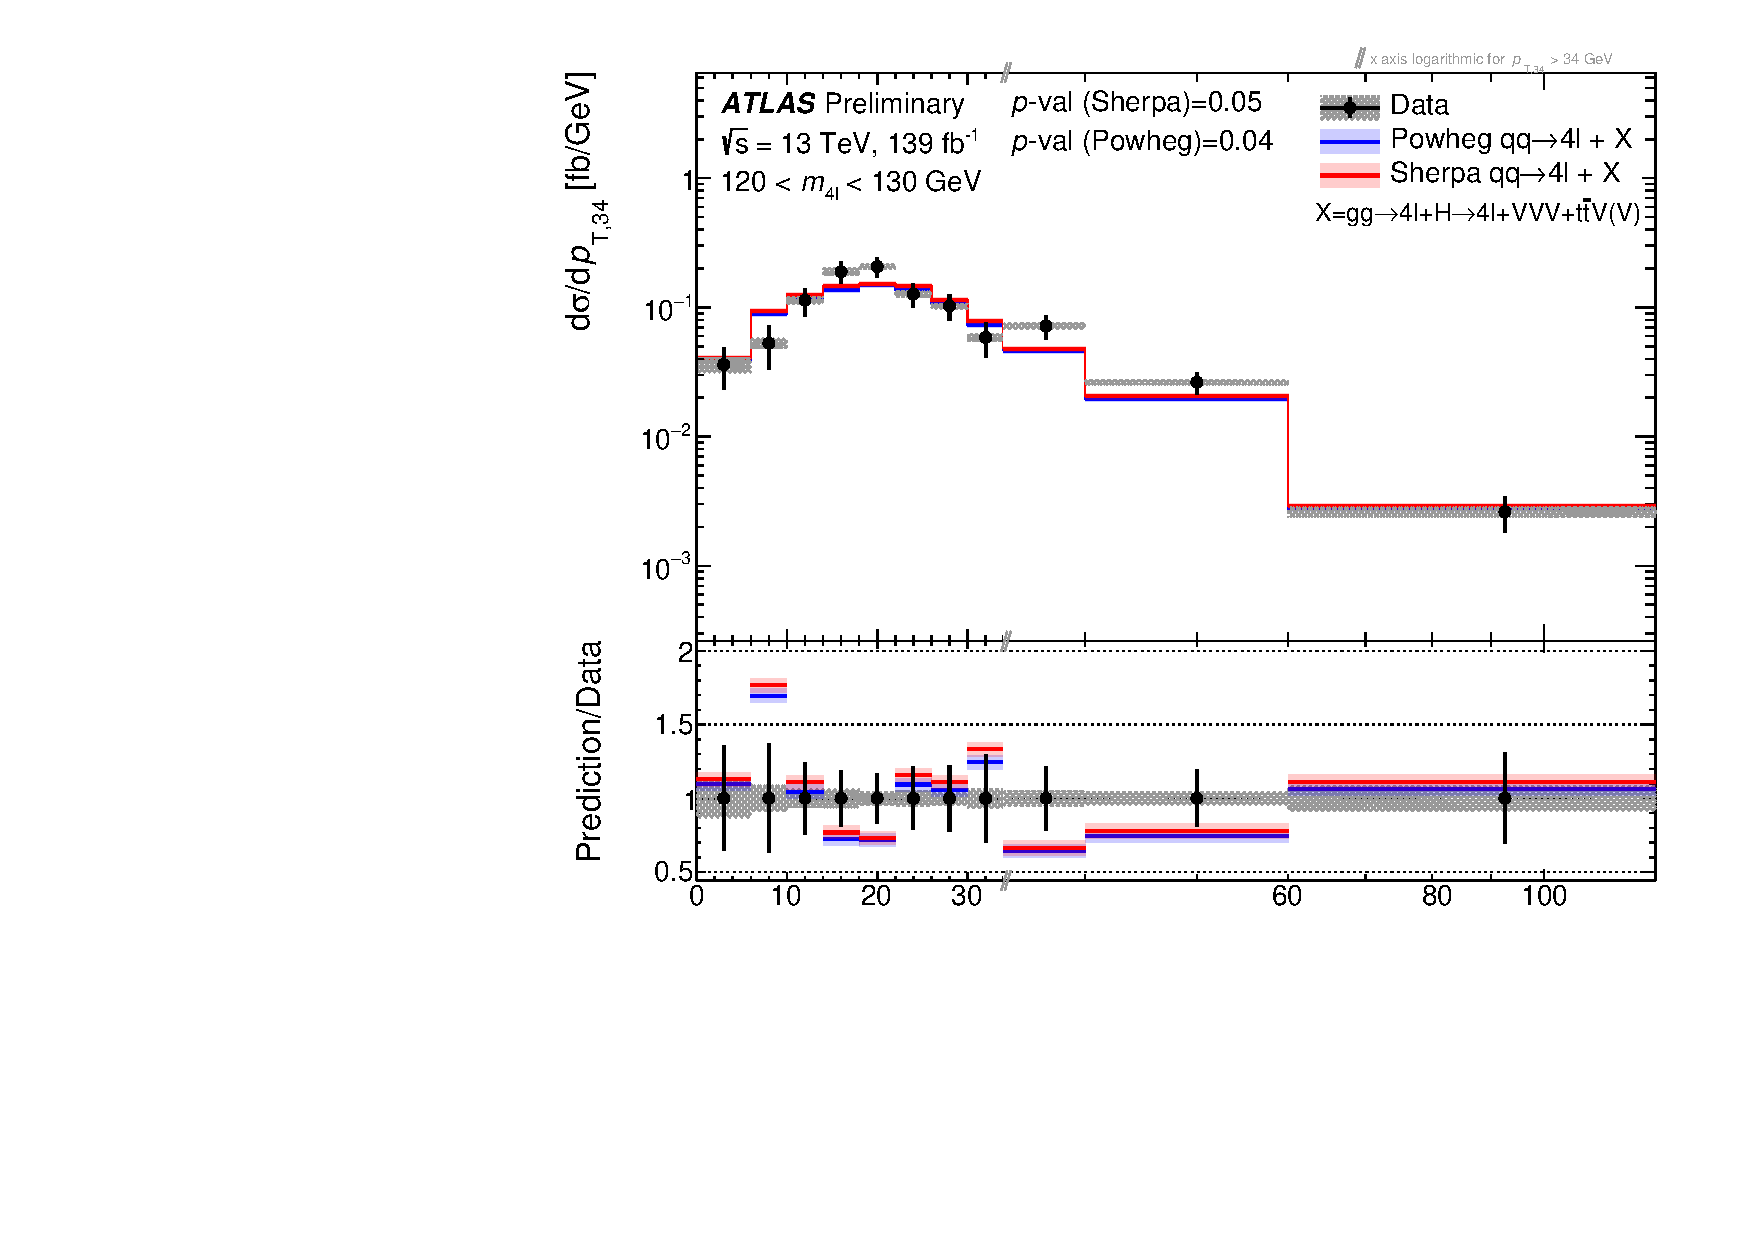
\includegraphics[width=.99\linewidth]{Figures/m4l/UnfoldedResults/linlog_Unfolded_Data_pt34_m4l120-130.pdf} \caption{\HFourL \ region}\label{fig:sub-second}
    \end{subfigure}
    \begin{subfigure}{.49\textwidth}\centering
      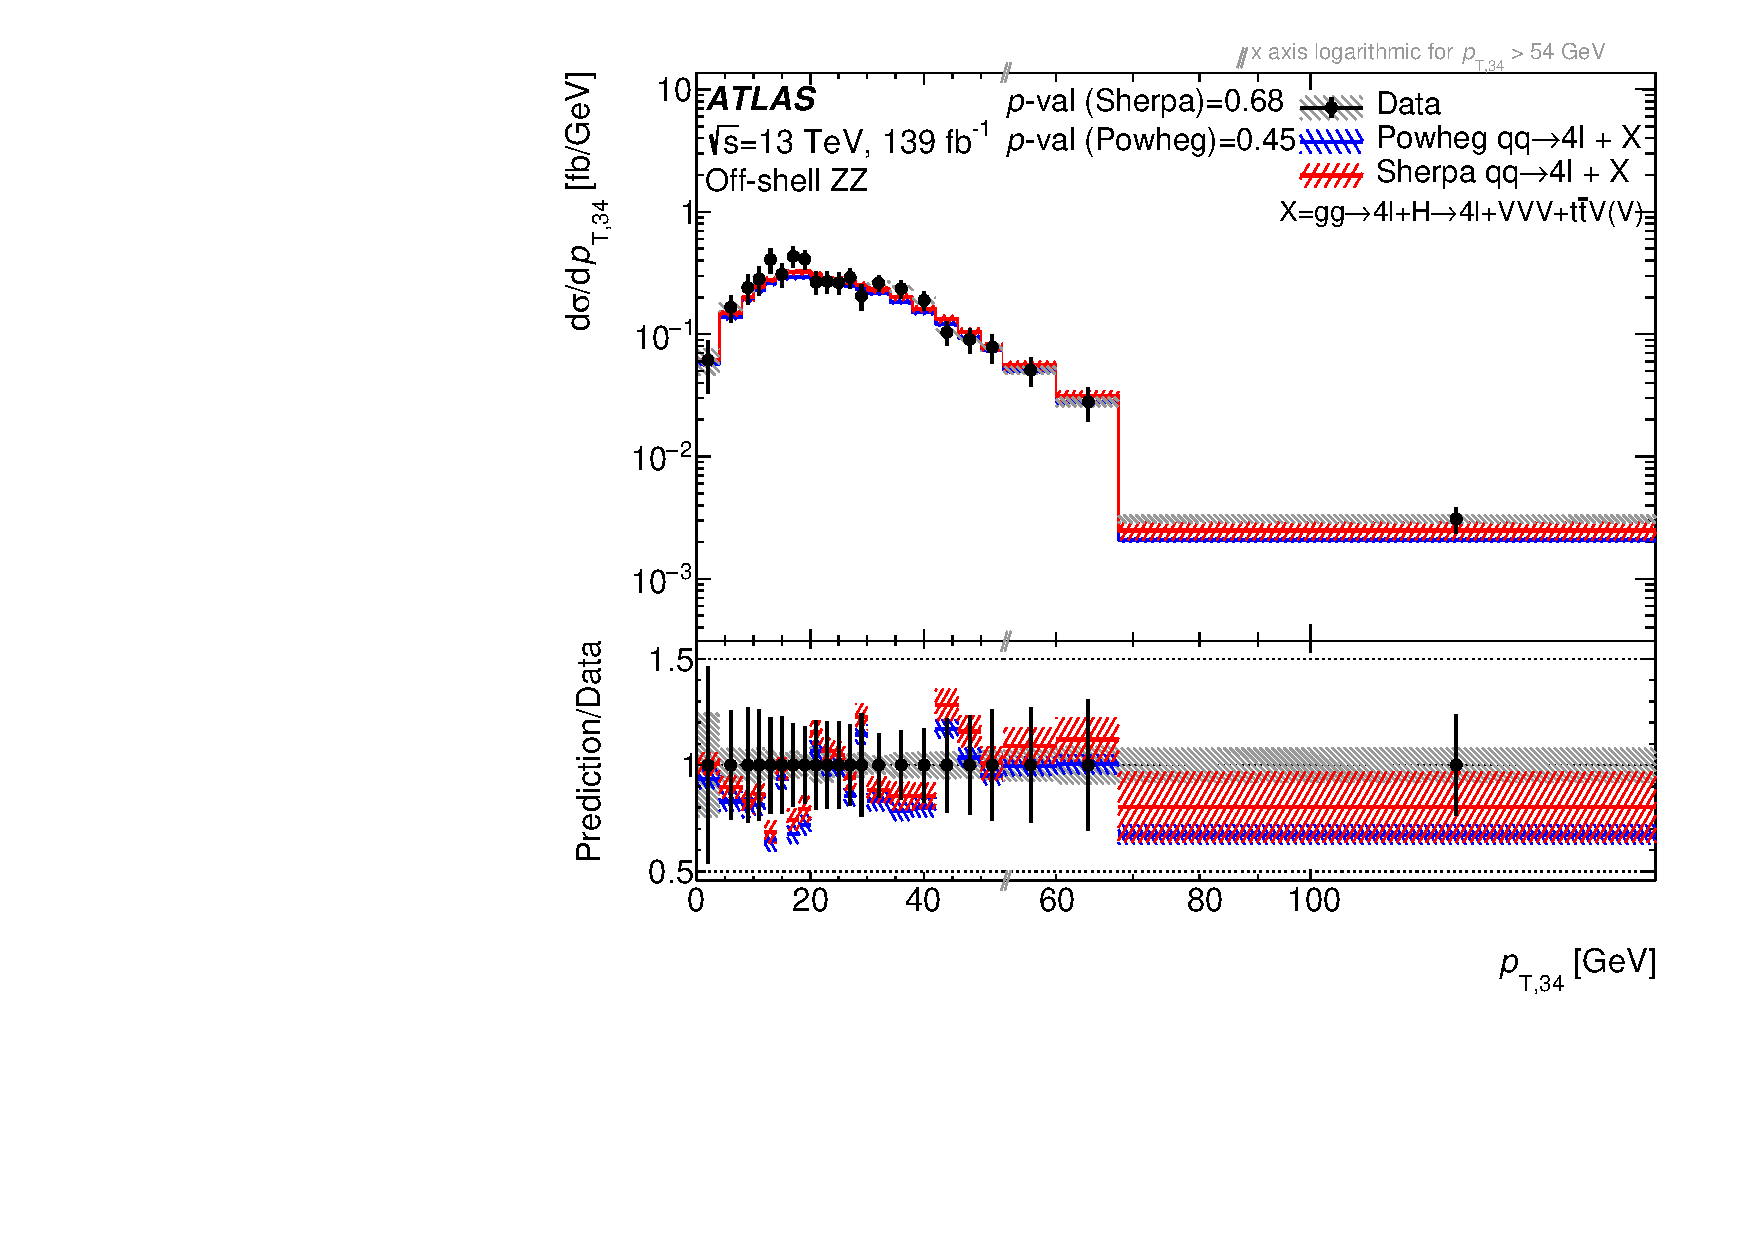
\includegraphics[width=.99\linewidth]{Figures/m4l/UnfoldedResults/linlog_Unfolded_Data_pt34_m4loffshell.pdf}  \caption{Off-shell $\Z\Z$ region}\label{fig:sub-third}
    \end{subfigure}
    \begin{subfigure}{.49\textwidth}\centering
      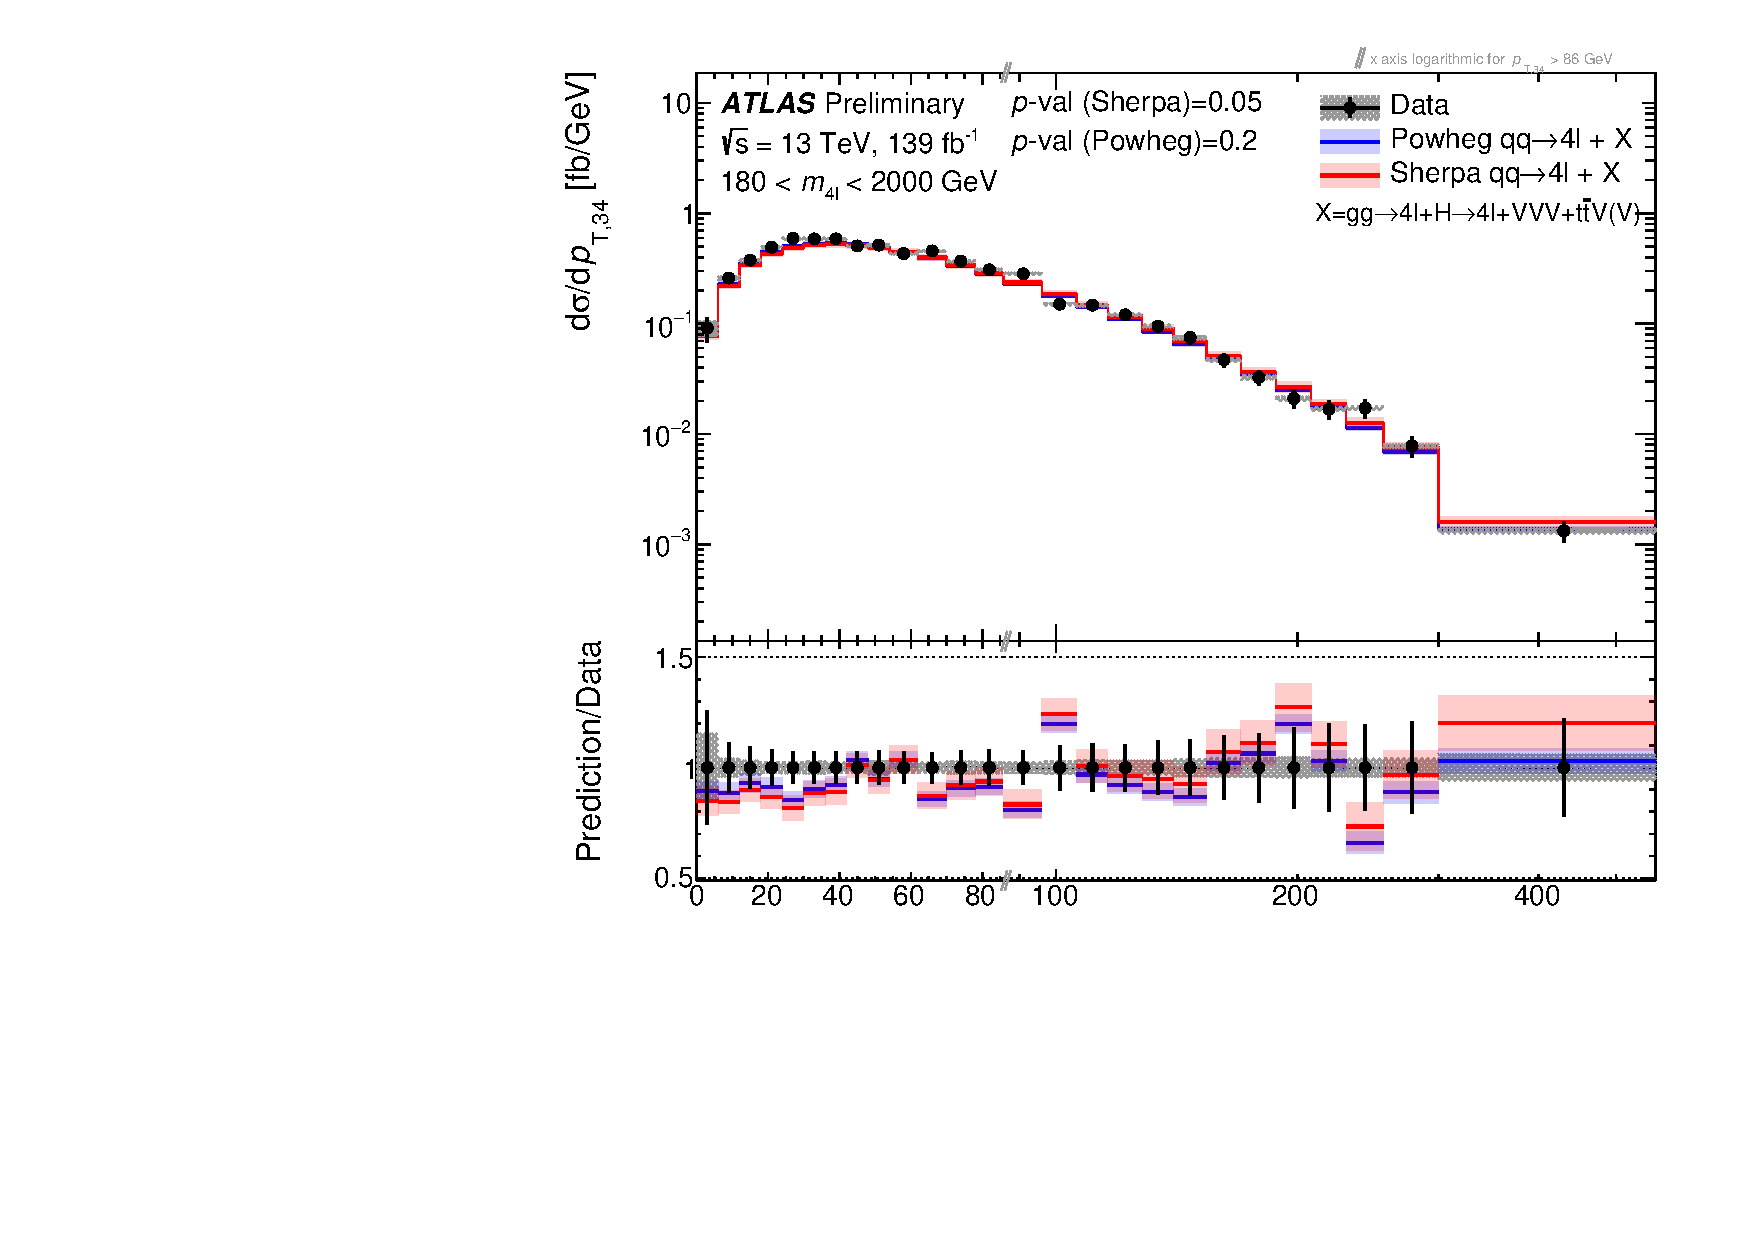
\includegraphics[width=.99\linewidth]{Figures/m4l/UnfoldedResults/linlog_Unfolded_Data_pt34_m4l180-2000.pdf}  \caption{On-shell $\Z\Z$ region}\label{fig:sub-fourth}
    \end{subfigure}
    \caption{Differential cross-section as a function of \ptZTwo{} in the four
        \mFourL{} regions. The measured data (black points) are  compared with the SM prediction using either \SHERPA{} (red, with red hashed band for the uncertainty) or \POWHEG{} + \pythia{} (blue, with blue hashed band for the uncertainty) to model the \qqFourL{} contribution. The error bars on the data points give the total uncertainty and the grey hashed band gives the systematic uncertainty. \Pvalue{} The  lower panel shows the ratio of the SM predictions to the data.}
    \label{fig:pt23_m4l}
\end{figure}

%% cosThetaStar1 vs m4l
\begin{figure}[htb!]
    \begin{subfigure}{.49\textwidth}\centering
      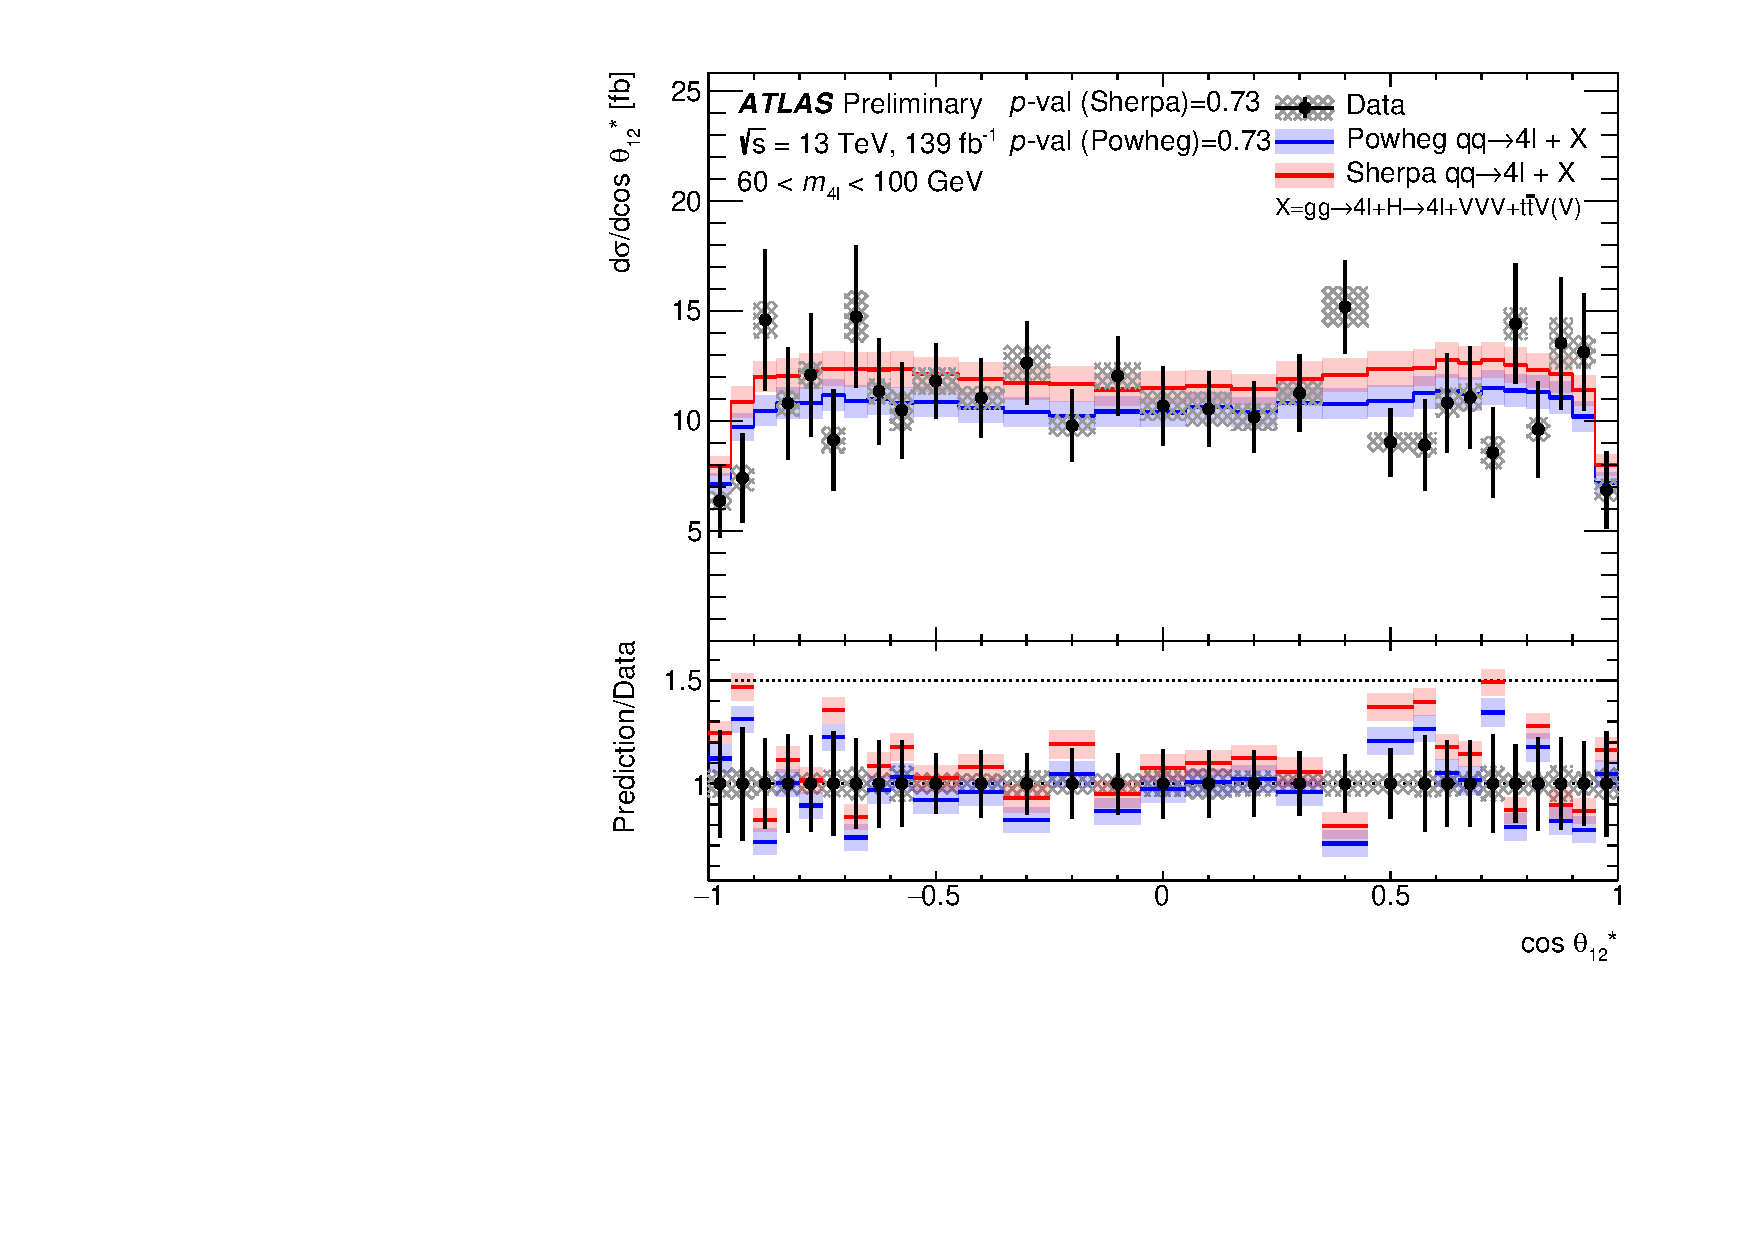
\includegraphics[width=.99\linewidth]{Figures/m4l/UnfoldedResults/linY_Unfolded_Data_cosThetaStar1_m4l60-100.pdf}\caption{\ZFourL \ region}\label{fig:sub-first}
    \end{subfigure}
    \begin{subfigure}{.49\textwidth}\centering
      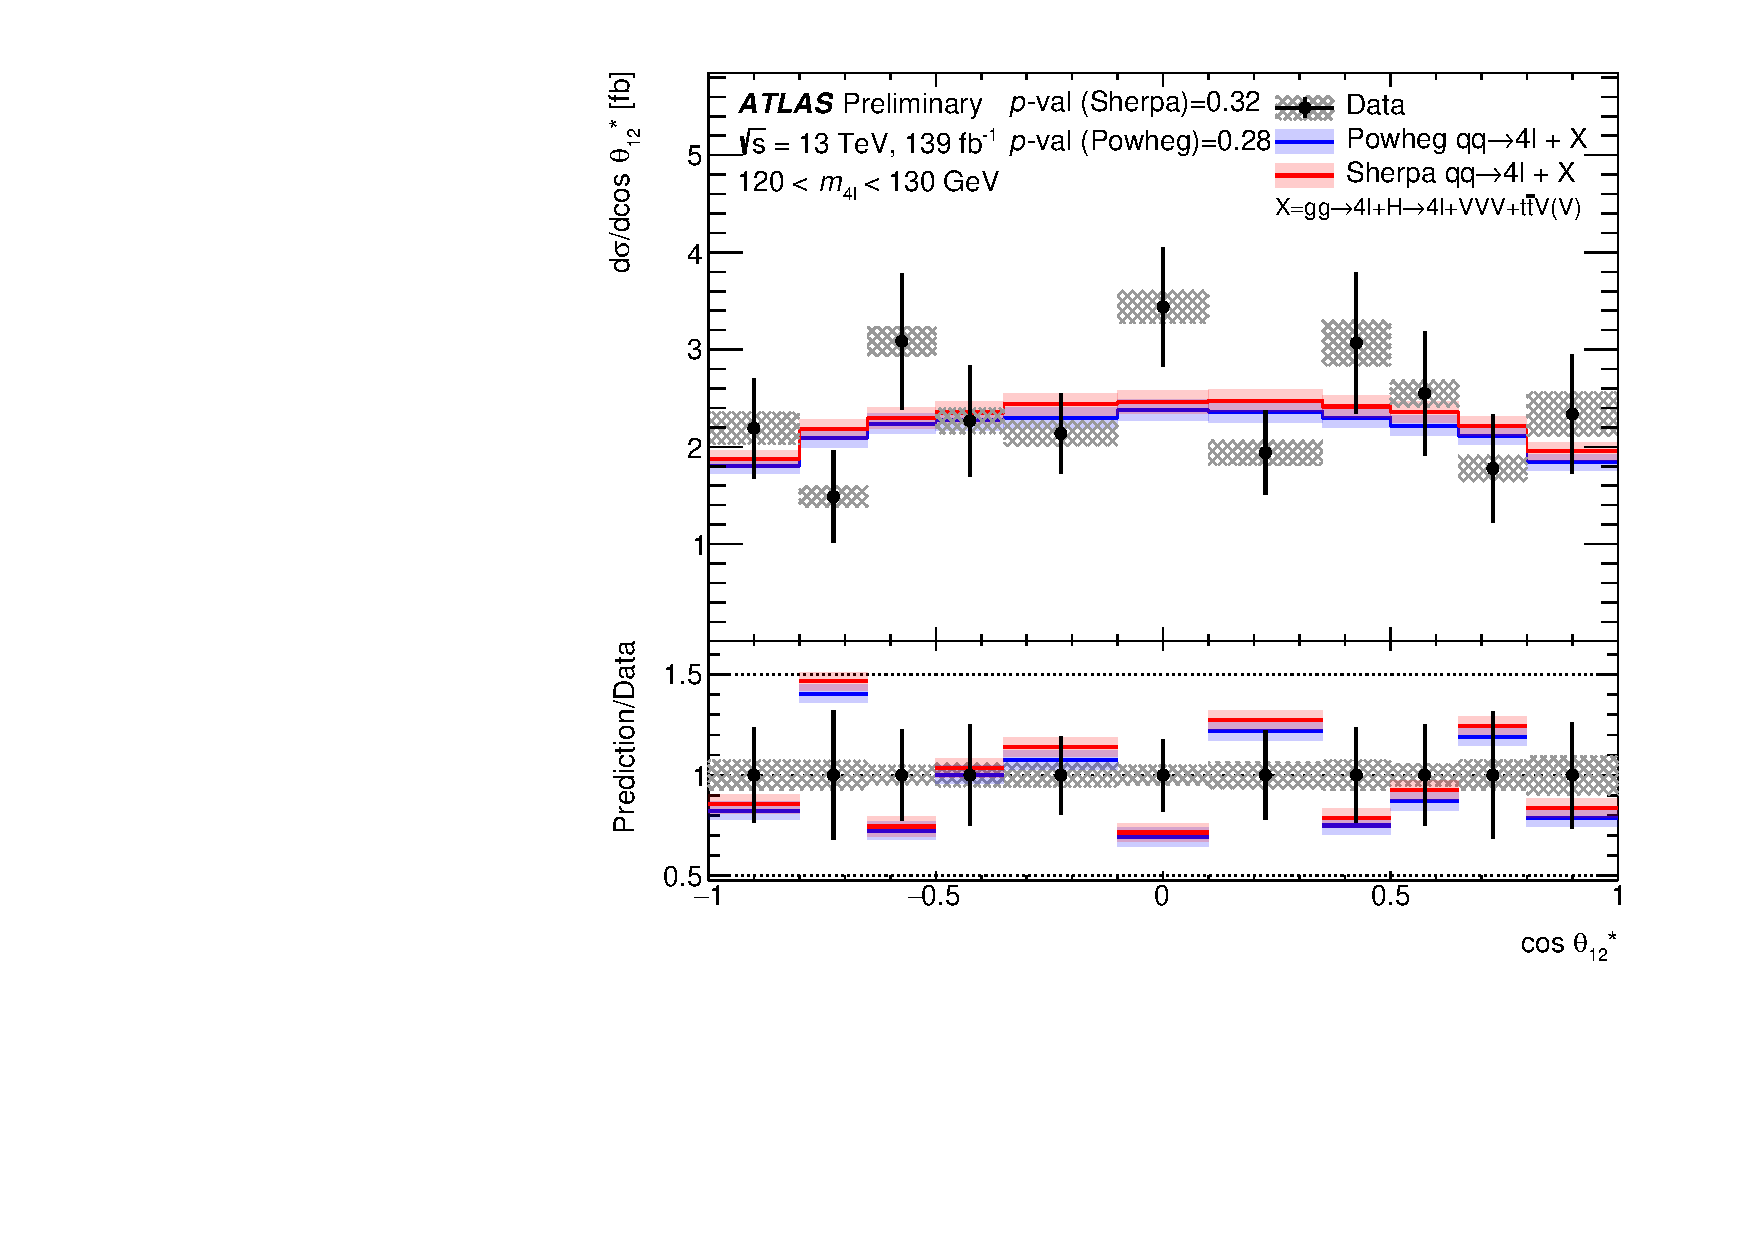
\includegraphics[width=.99\linewidth]{Figures/m4l/UnfoldedResults/linY_Unfolded_Data_cosThetaStar1_m4l120-130.pdf} \caption{\HFourL \ region}\label{fig:sub-second}
    \end{subfigure}
    \begin{subfigure}{.49\textwidth}\centering
      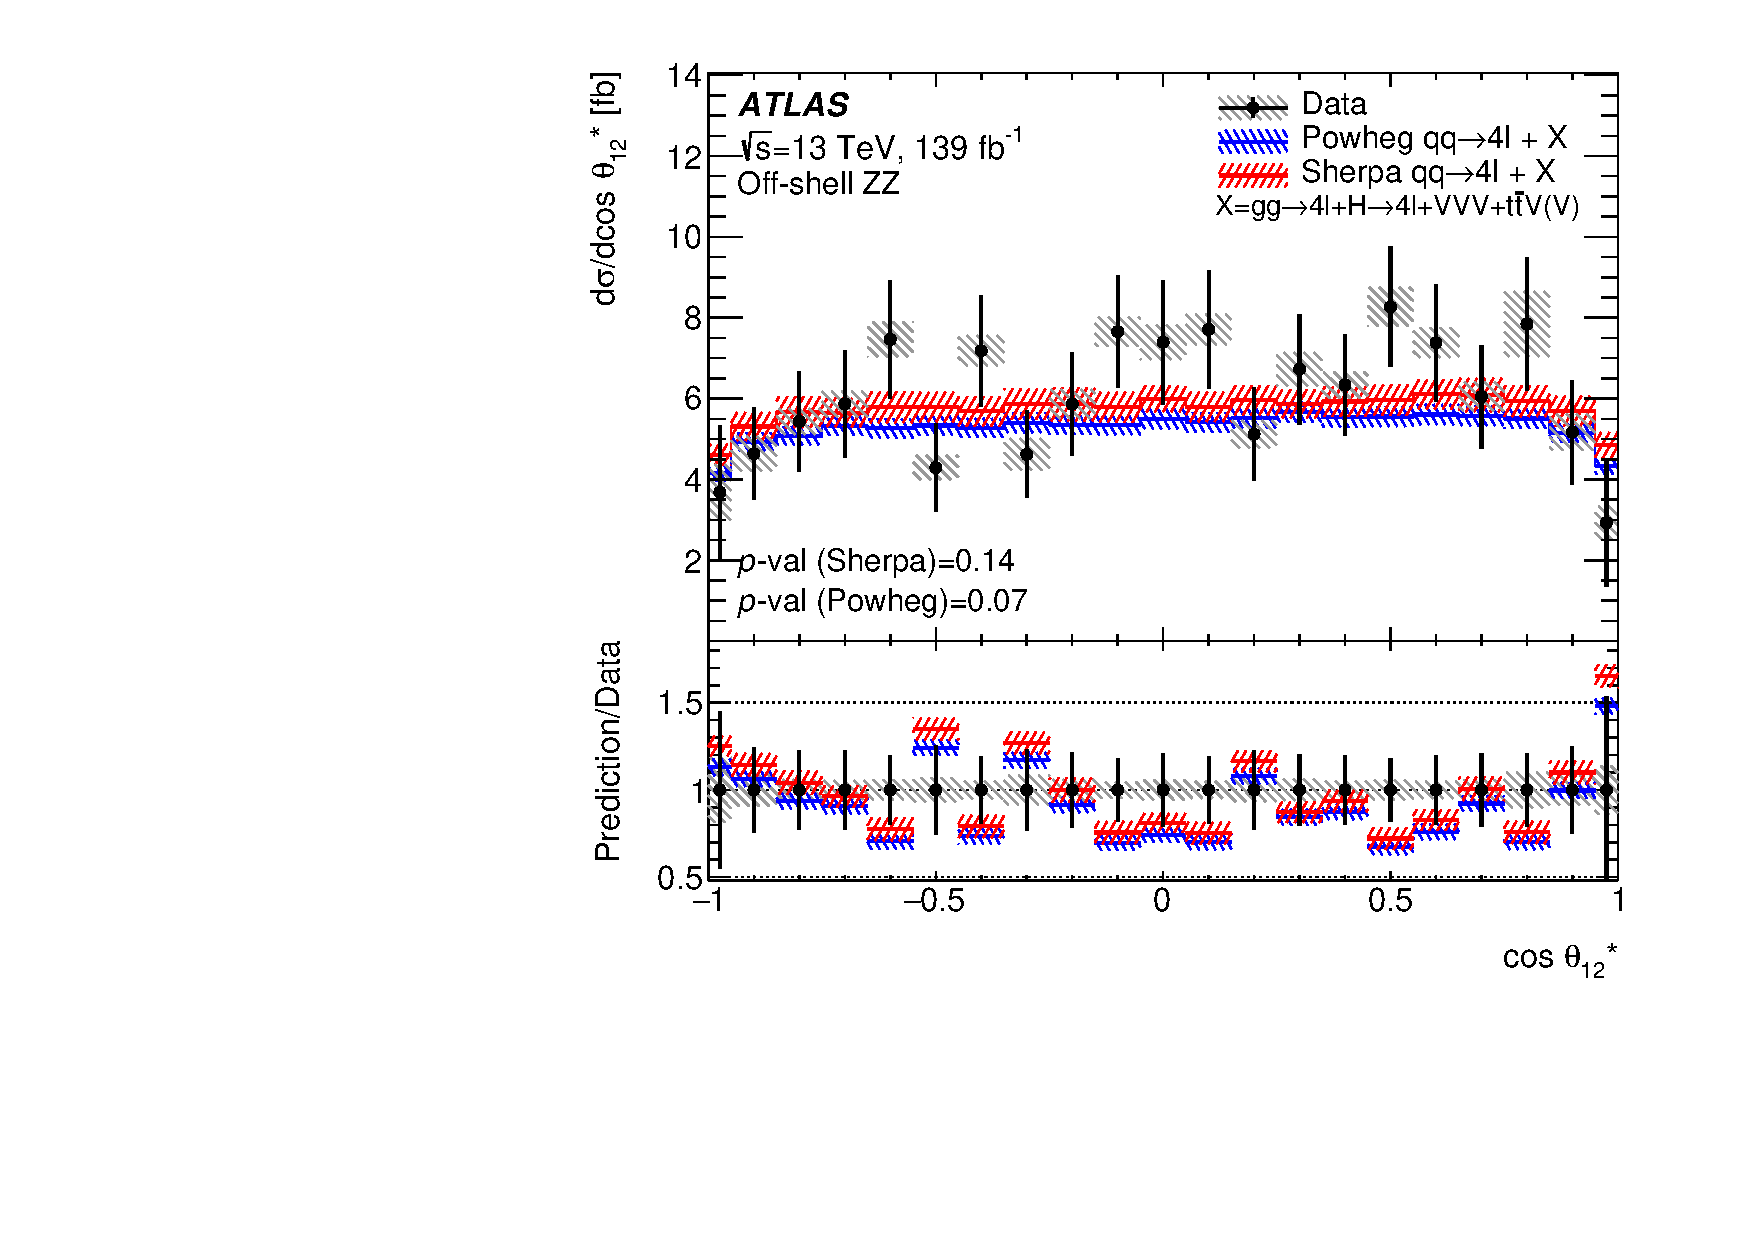
\includegraphics[width=.99\linewidth]{Figures/m4l/UnfoldedResults/linY_Unfolded_Data_cosThetaStar1_m4loffshell.pdf}  \caption{Off-shell $\Z\Z$ region}\label{fig:sub-third}
    \end{subfigure}
    \begin{subfigure}{.49\textwidth}\centering
      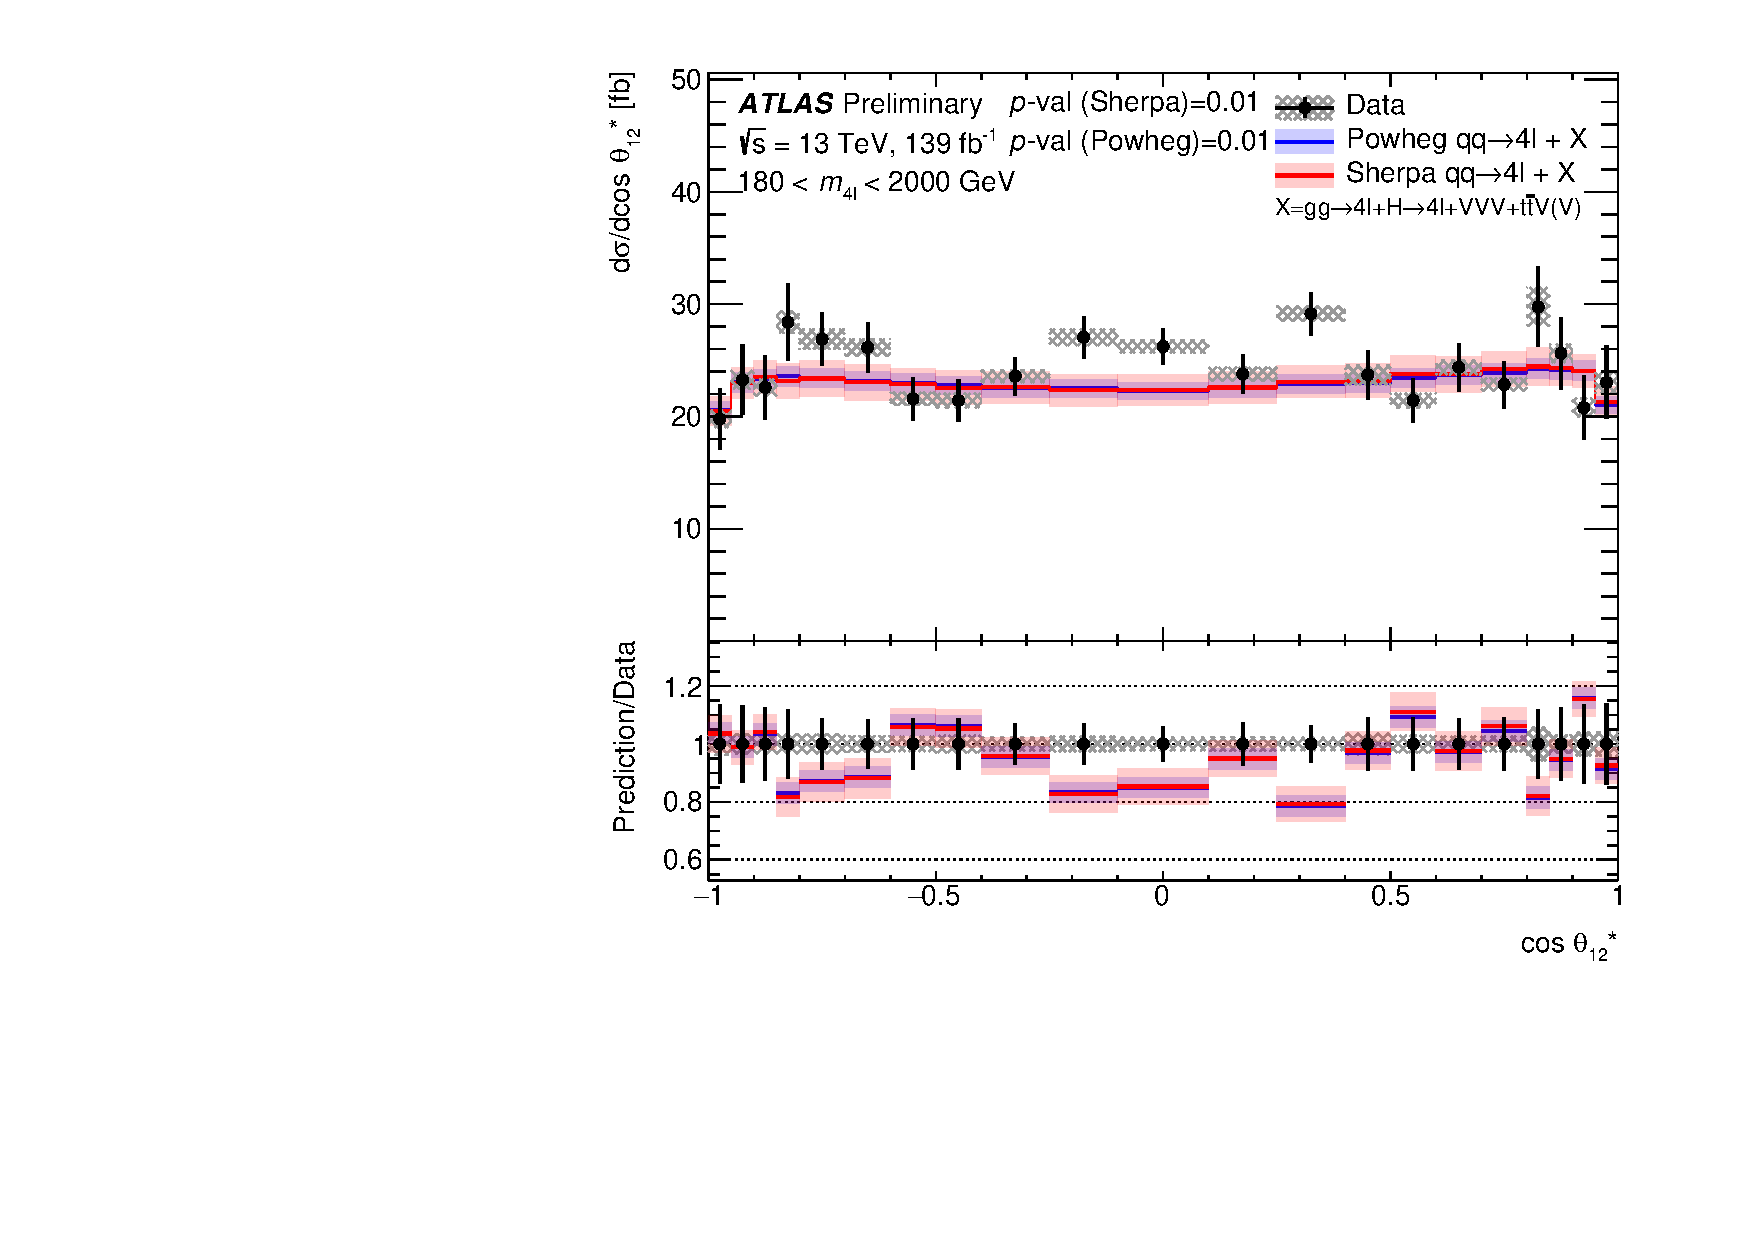
\includegraphics[width=.99\linewidth]{Figures/m4l/UnfoldedResults/linY_Unfolded_Data_cosThetaStar1_m4l180-2000.pdf}  \caption{On-shell $\Z\Z$ region}\label{fig:sub-fourth}
    \end{subfigure}
    \caption{Differential cross-section as a function of \CTSOneTwo{} in the four
        \mFourL{} regions. The measured data (black points) are  compared with the SM prediction using either \SHERPA{} (red, with red hashed band for the uncertainty) or \POWHEG{} + \pythia{} (blue, with blue hashed band for the uncertainty) to model the \qqFourL{} contribution. The error bars on the data points give the total uncertainty and the grey hashed band gives the systematic uncertainty. \Pvalue{} The  lower panel shows the ratio of the SM predictions to the data.}
    \label{fig:cts12_m4l}
\end{figure}

%% cosThetaStar3 vs m4l
\begin{figure}[htb!]
    \begin{subfigure}{.49\textwidth}\centering
      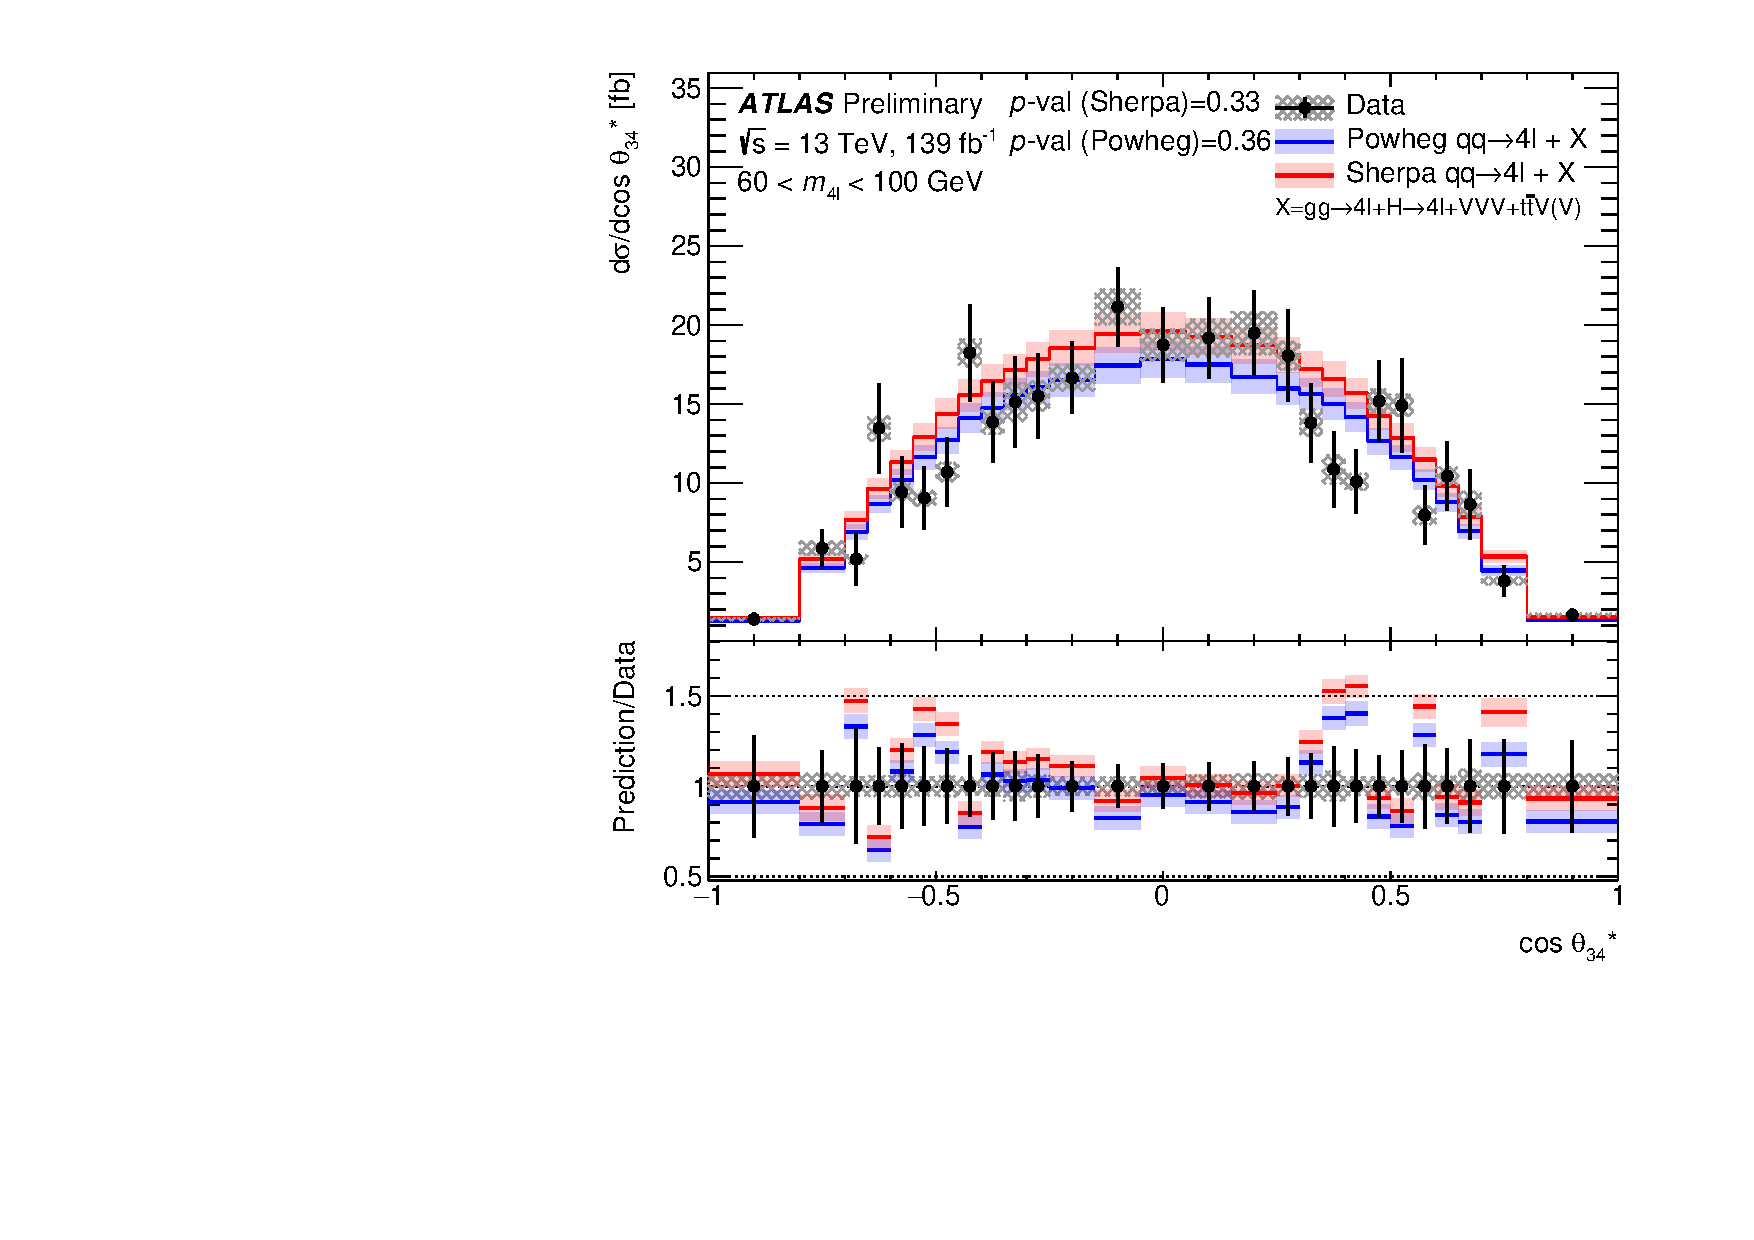
\includegraphics[width=.99\linewidth]{Figures/m4l/UnfoldedResults/linY_Unfolded_Data_cosThetaStar3_m4l60-100.pdf}\caption{\ZFourL \ region}\label{fig:sub-first}
    \end{subfigure}
    \begin{subfigure}{.49\textwidth}\centering
      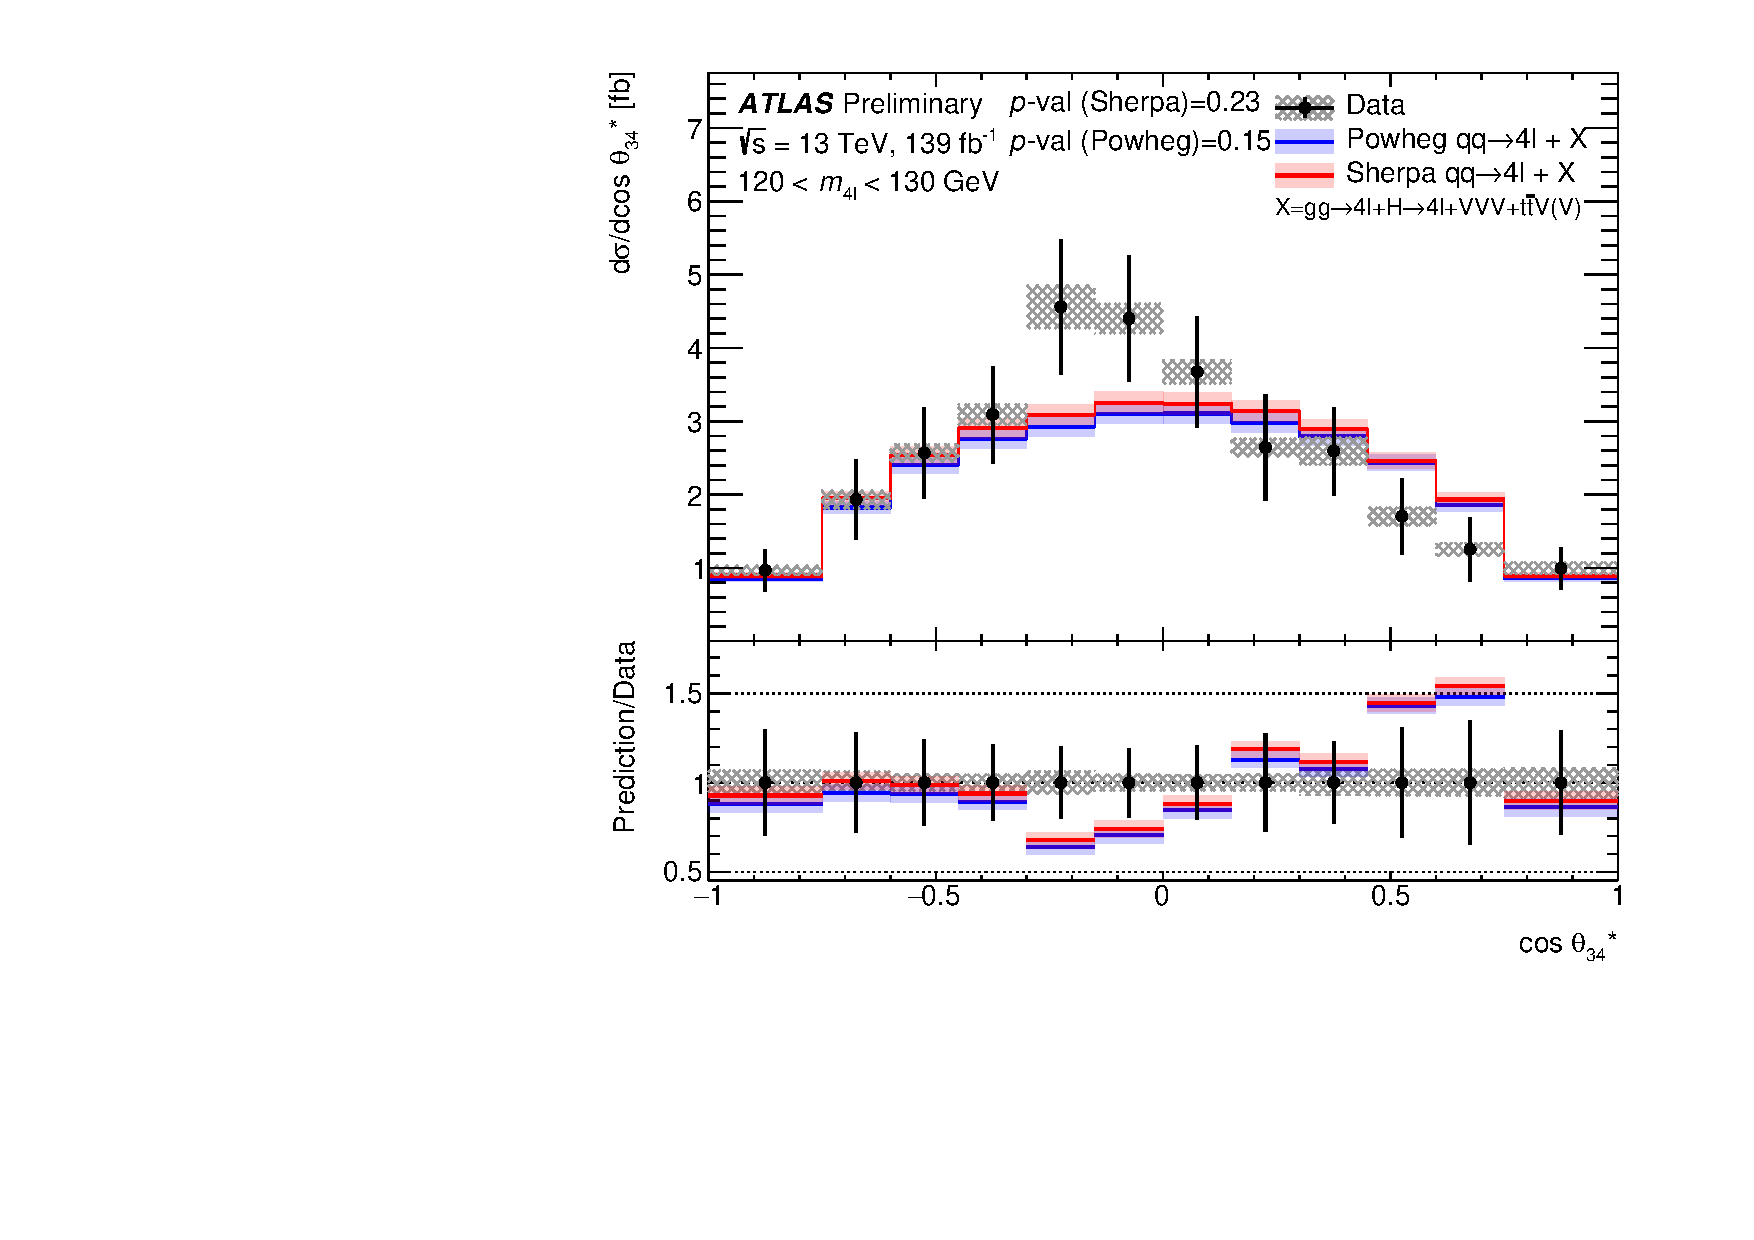
\includegraphics[width=.99\linewidth]{Figures/m4l/UnfoldedResults/linY_Unfolded_Data_cosThetaStar3_m4l120-130.pdf} \caption{\HFourL \ region}\label{fig:sub-second}
    \end{subfigure}
    \begin{subfigure}{.49\textwidth}\centering
      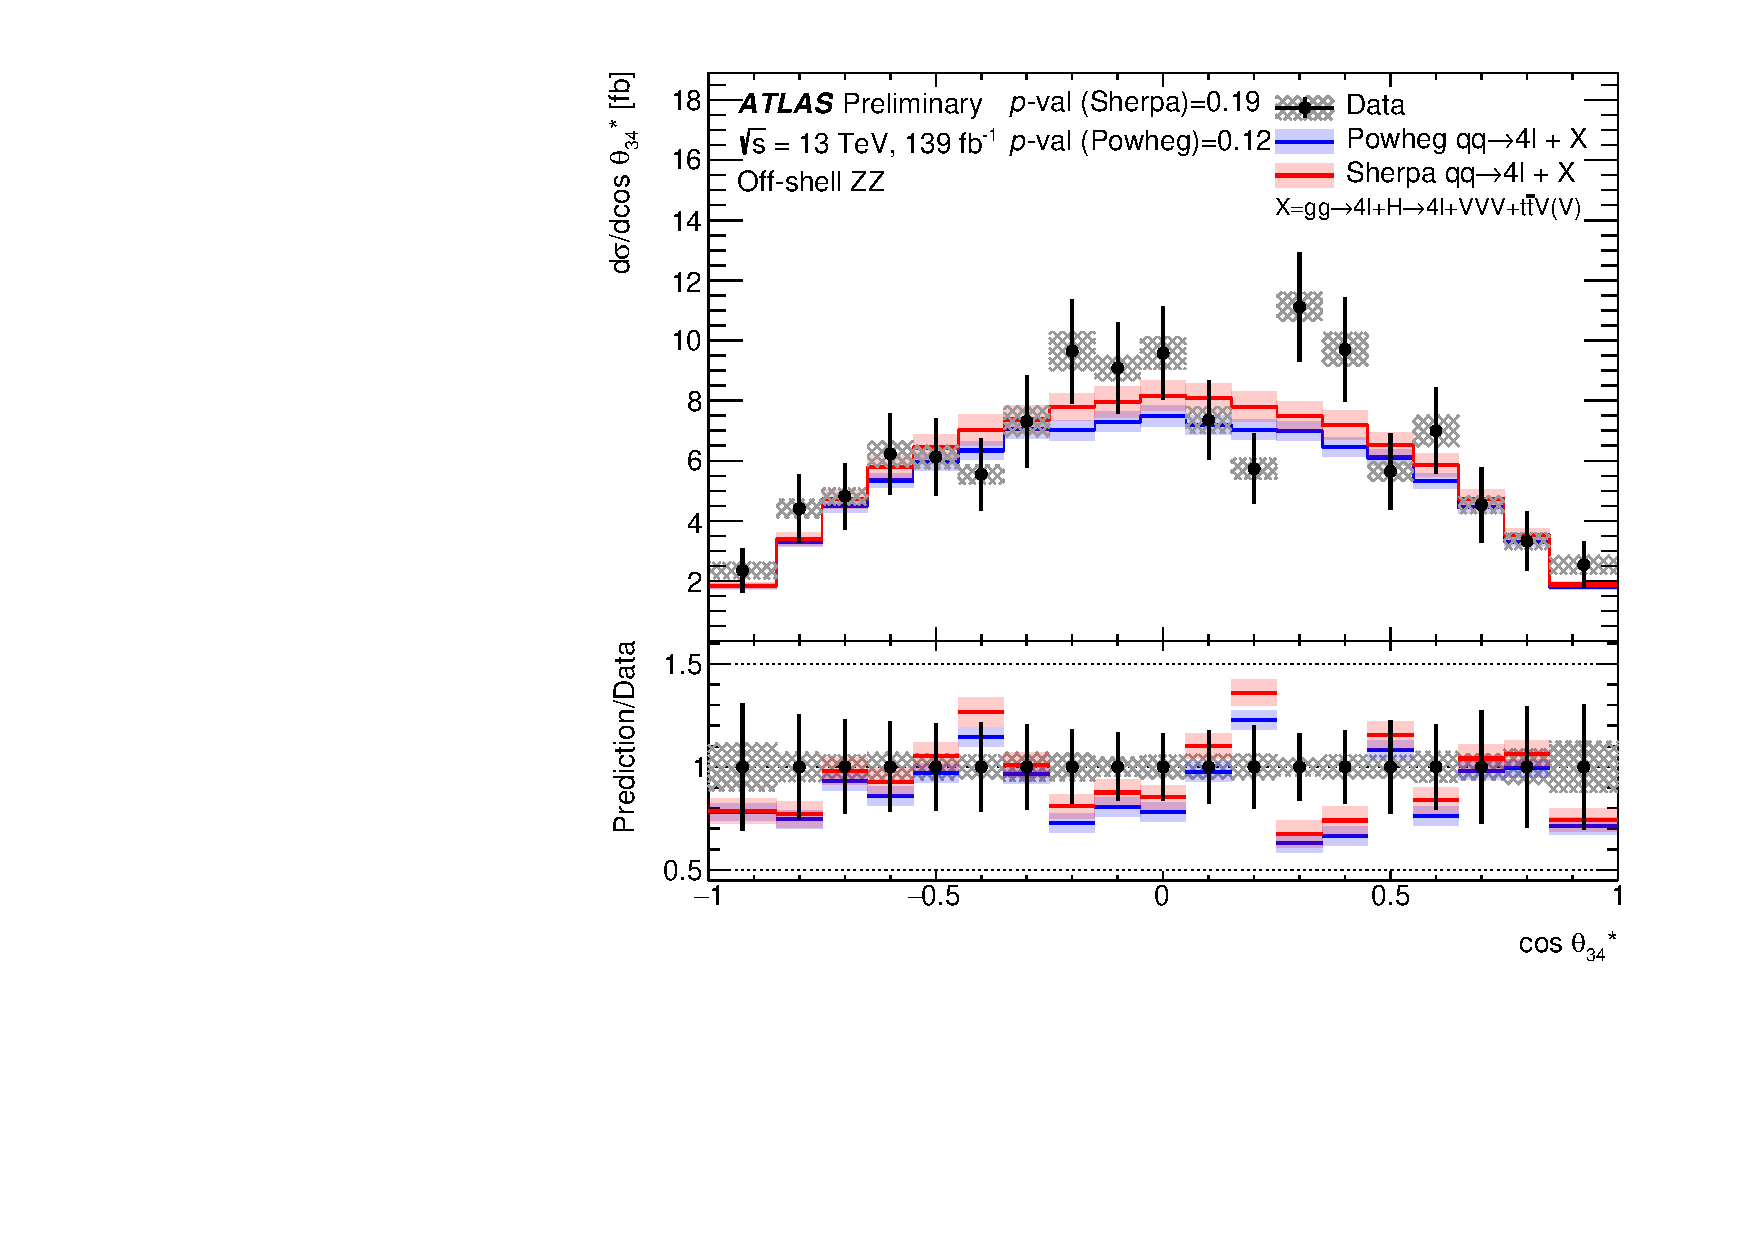
\includegraphics[width=.99\linewidth]{Figures/m4l/UnfoldedResults/linY_Unfolded_Data_cosThetaStar3_m4loffshell.pdf}  \caption{Off-shell $\Z\Z$ region}\label{fig:sub-third}
    \end{subfigure}
    \begin{subfigure}{.49\textwidth}\centering
      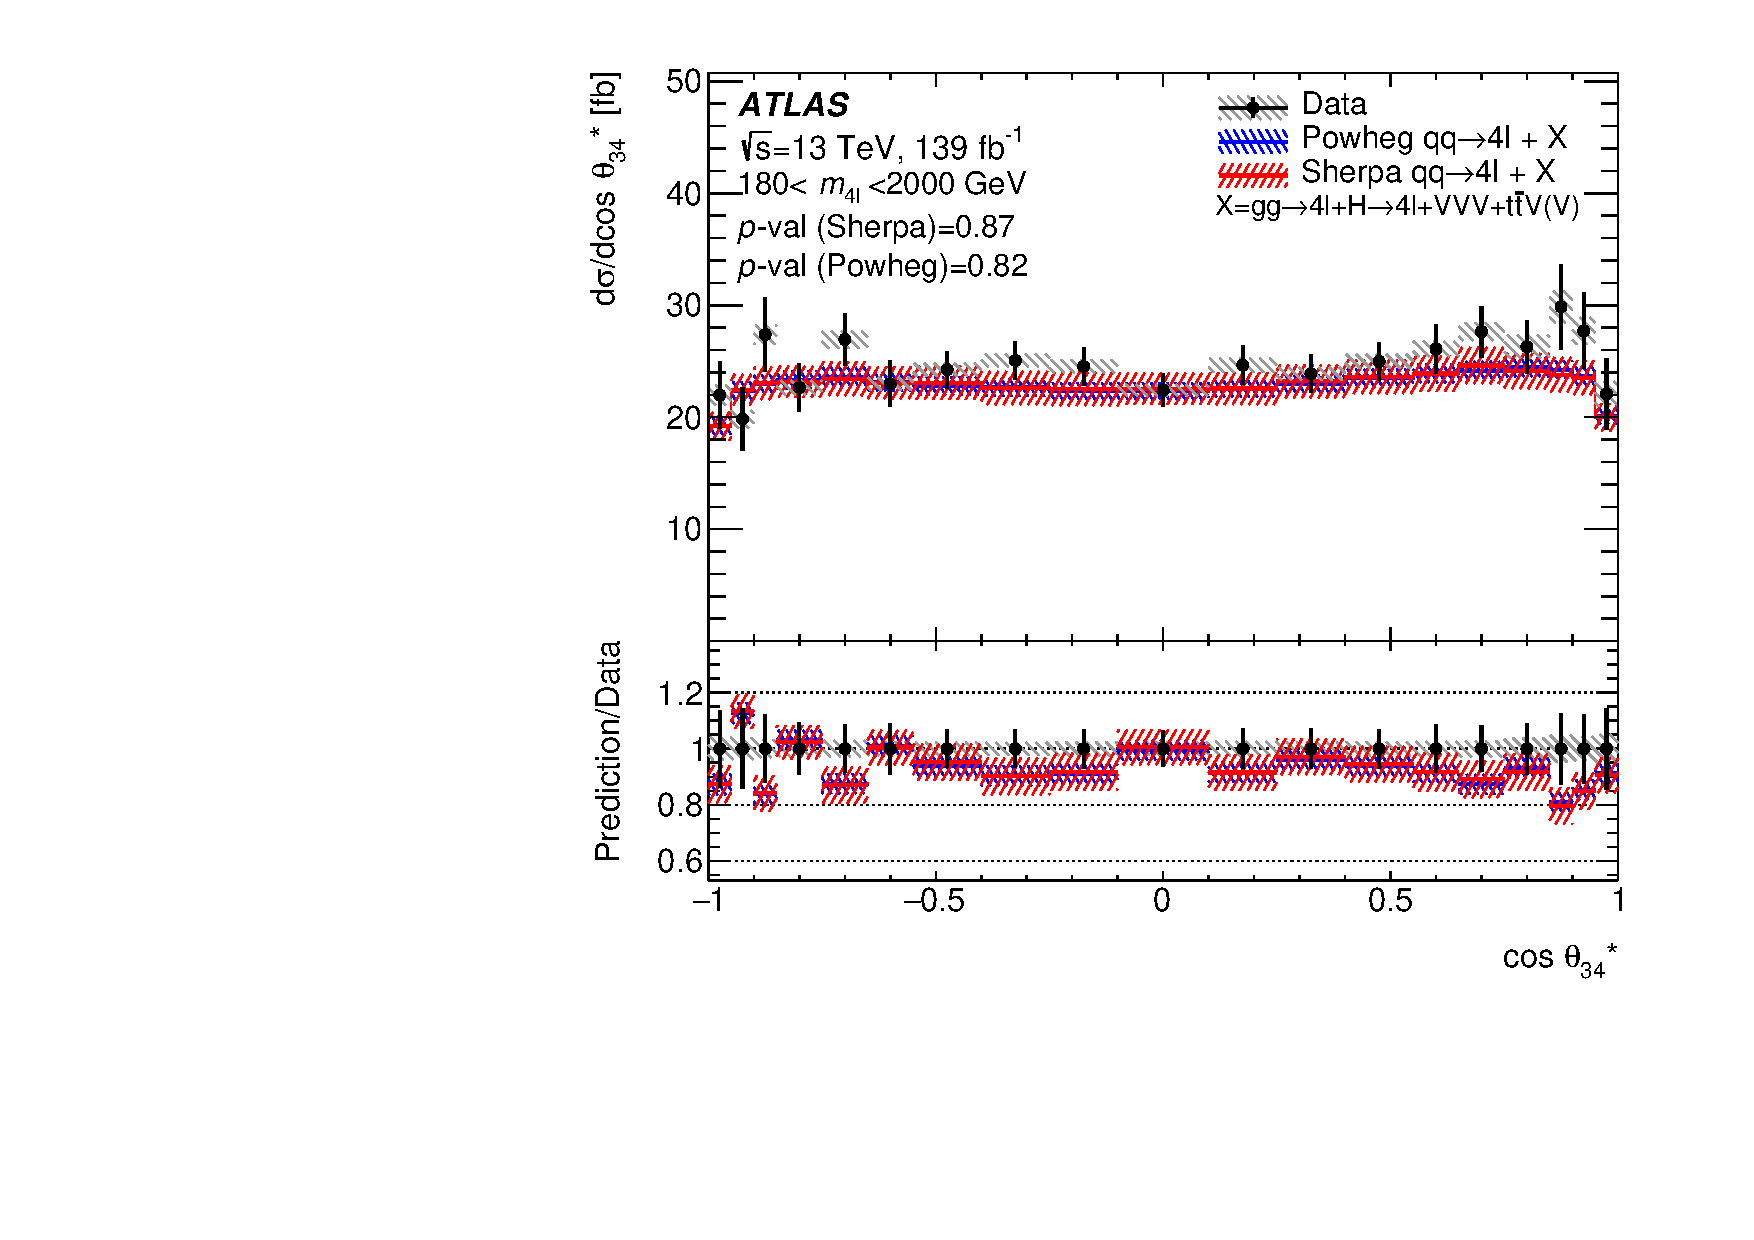
\includegraphics[width=.99\linewidth]{Figures/m4l/UnfoldedResults/linY_Unfolded_Data_cosThetaStar3_m4l180-2000.pdf}  \caption{On-shell $\Z\Z$ region}\label{fig:sub-fourth}
    \end{subfigure}
    \caption{Differential cross-section as a function of \CTSThreeFour{} in the four
        \mFourL{} regions. The measured data (black points) are  compared with the SM prediction using either \SHERPA{} (red, with red hashed band for the uncertainty) or \POWHEG{} + \pythia{} (blue, with blue hashed band for the uncertainty) to model the \qqFourL{} contribution. The error bars on the data points give the total uncertainty and the grey hashed band gives the systematic uncertainty. \Pvalue{} The  lower panel shows the ratio of the SM predictions to the data.}
    \label{fig:cts34_m4l}
\end{figure}

%% deltaPhiLeptons vs m4l
\begin{figure}[htb!]
    \begin{subfigure}{.49\textwidth}\centering
      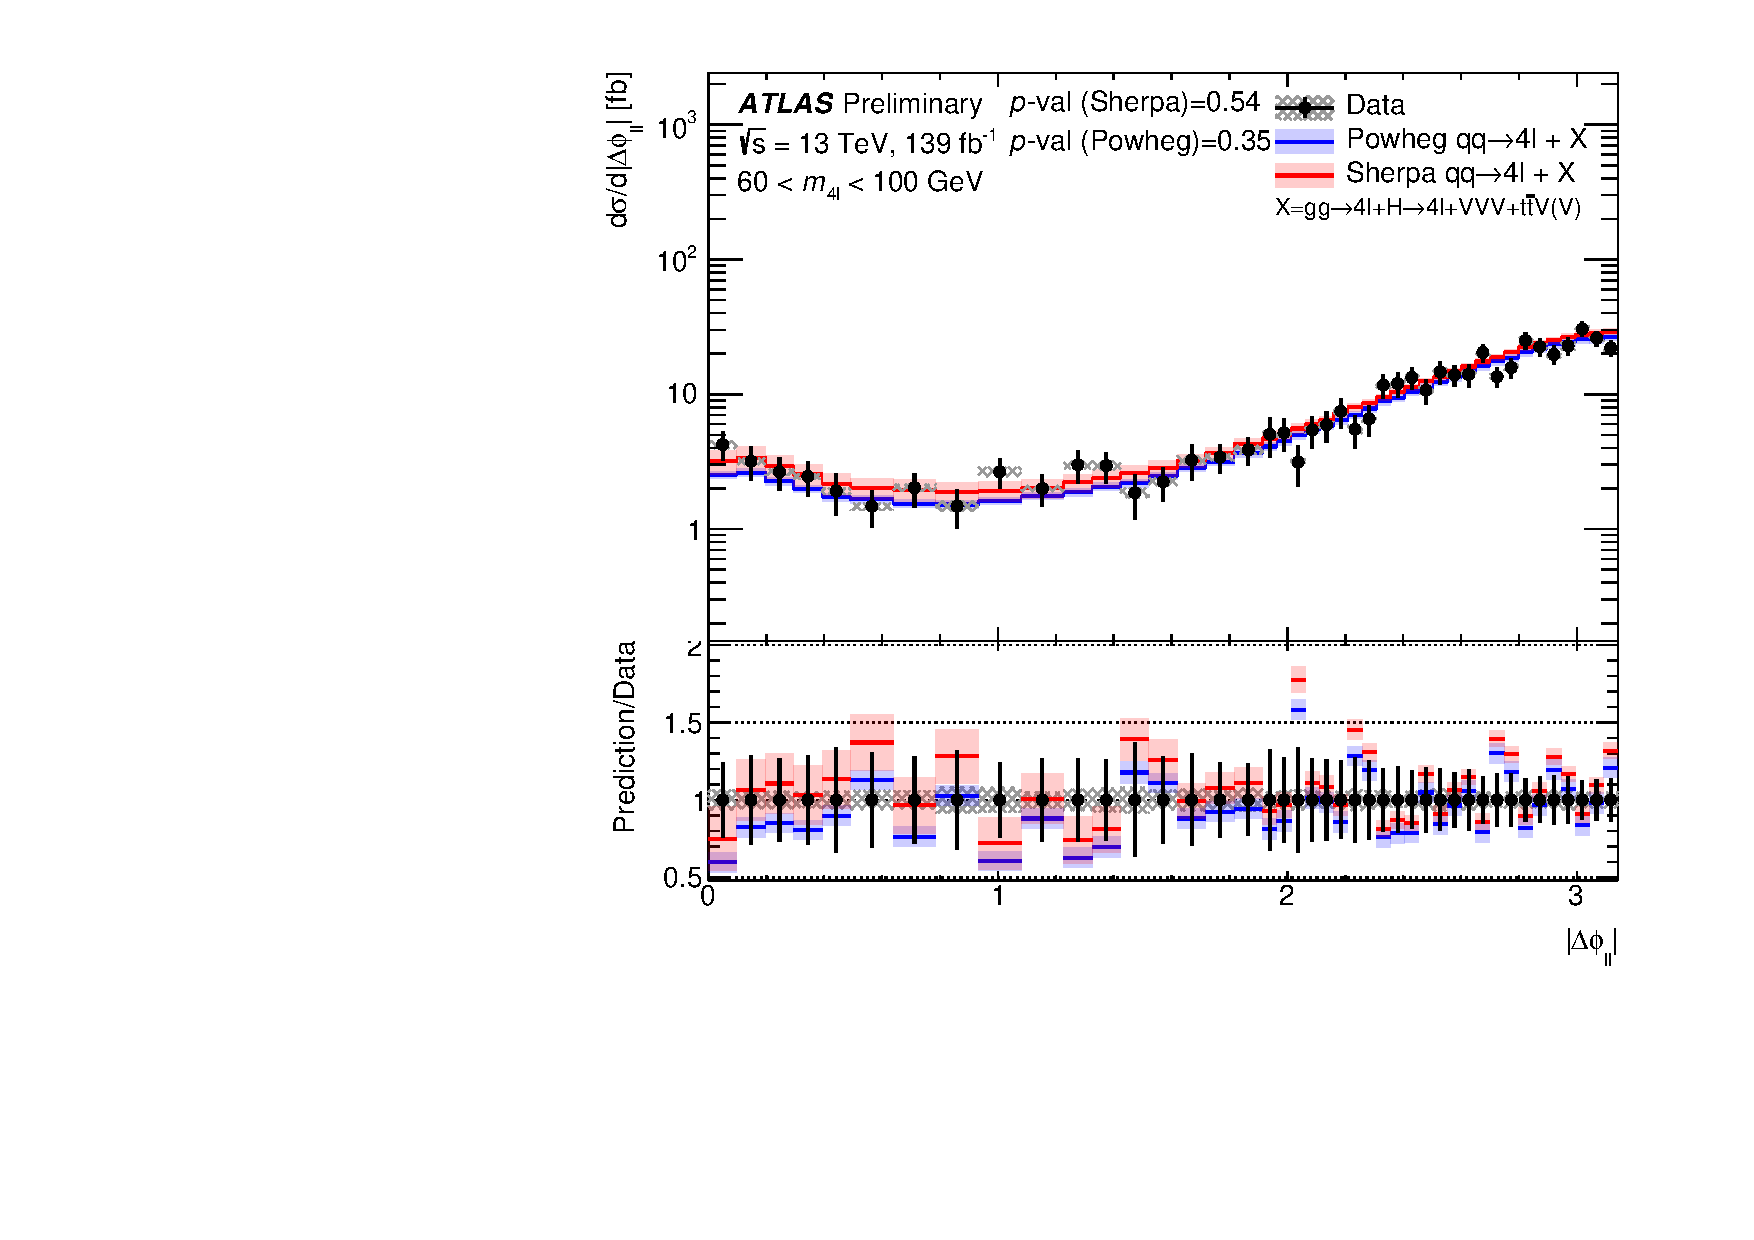
\includegraphics[width=.99\linewidth]{Figures/m4l/UnfoldedResults/Unfolded_Data_deltaPhiLeadingLeptons_m4l60-100.pdf}\caption{\ZFourL \ region}\label{fig:sub-first}
    \end{subfigure}
    \begin{subfigure}{.49\textwidth}\centering
      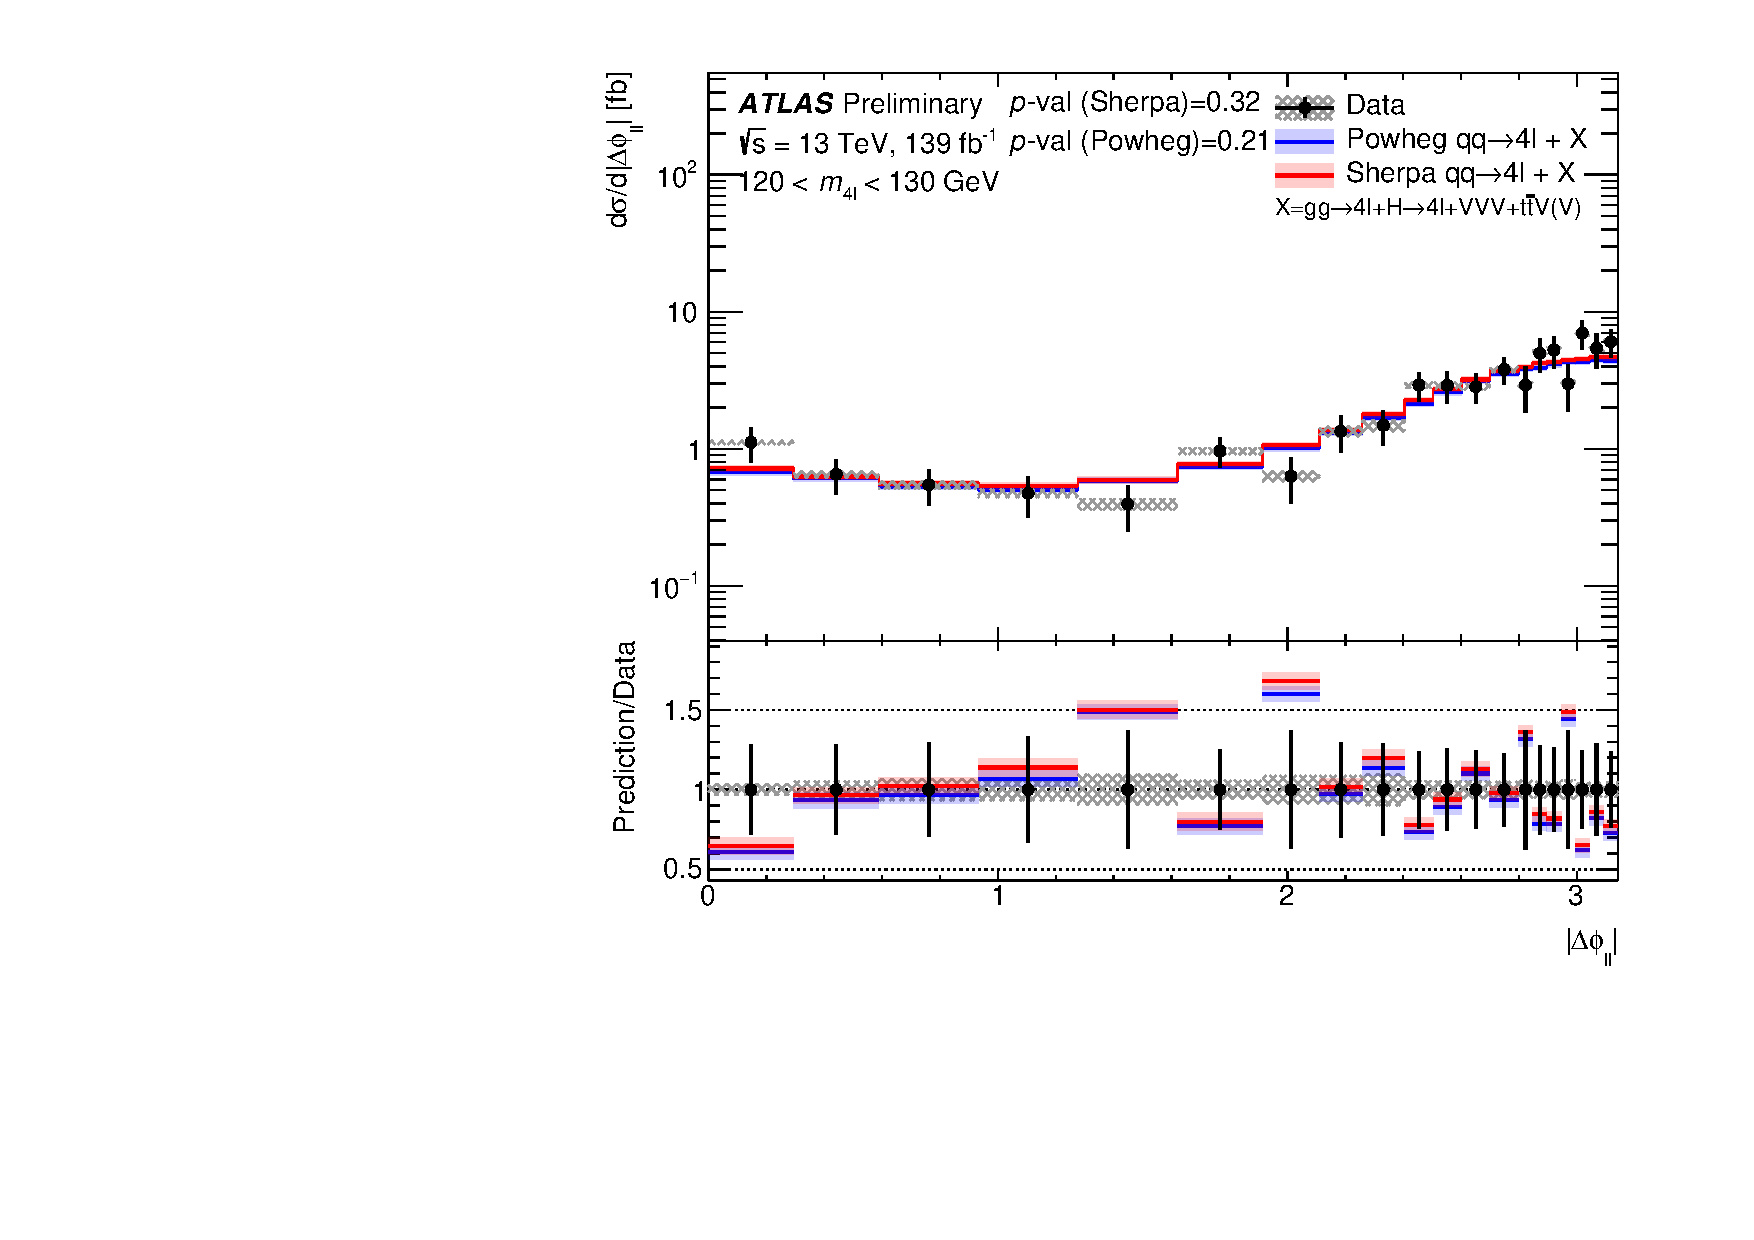
\includegraphics[width=.99\linewidth]{Figures/m4l/UnfoldedResults/Unfolded_Data_deltaPhiLeadingLeptons_m4l120-130.pdf} \caption{\HFourL \ region}\label{fig:sub-second}
    \end{subfigure}
    \begin{subfigure}{.49\textwidth}\centering
      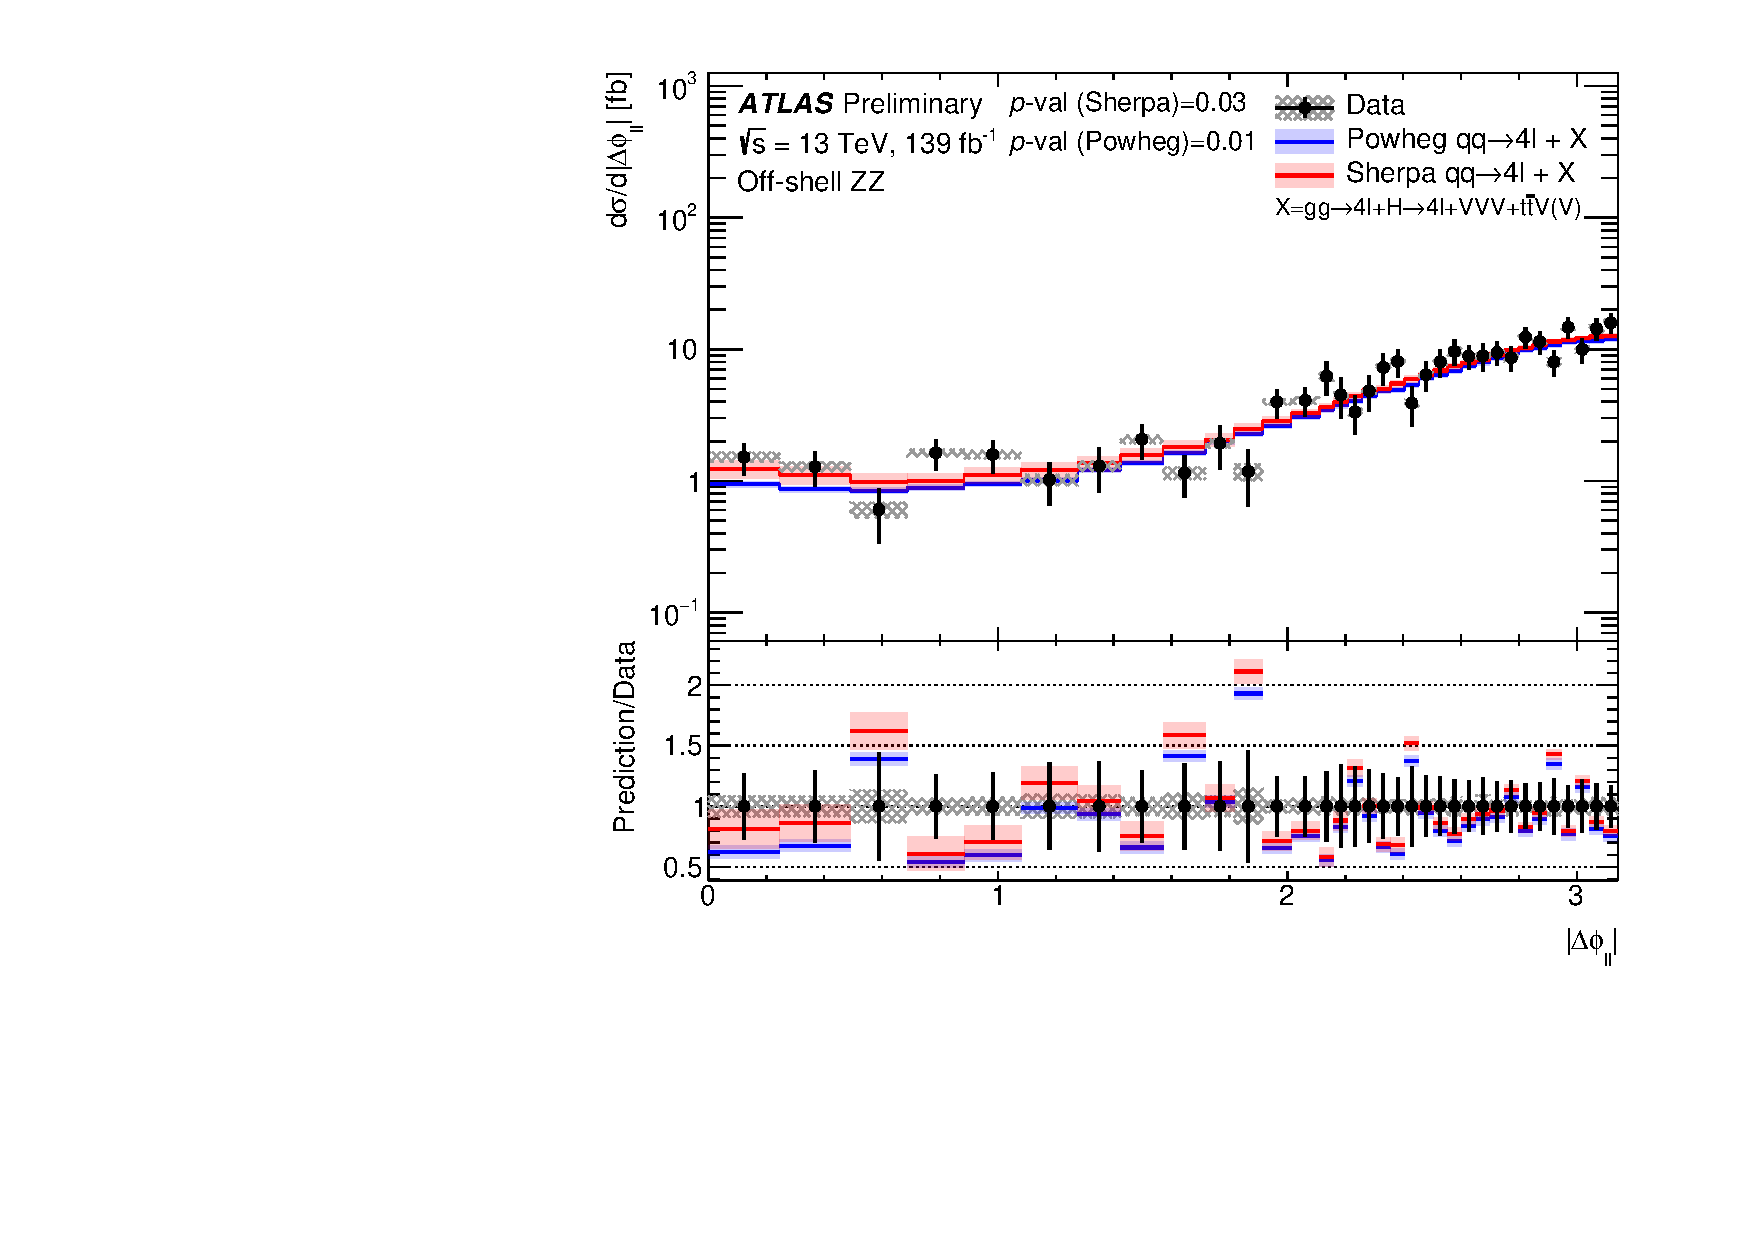
\includegraphics[width=.99\linewidth]{Figures/m4l/UnfoldedResults/Unfolded_Data_deltaPhiLeadingLeptons_m4loffshell.pdf}  \caption{Off-shell $\Z\Z$ region}\label{fig:sub-third}
    \end{subfigure}
    \begin{subfigure}{.49\textwidth}\centering
      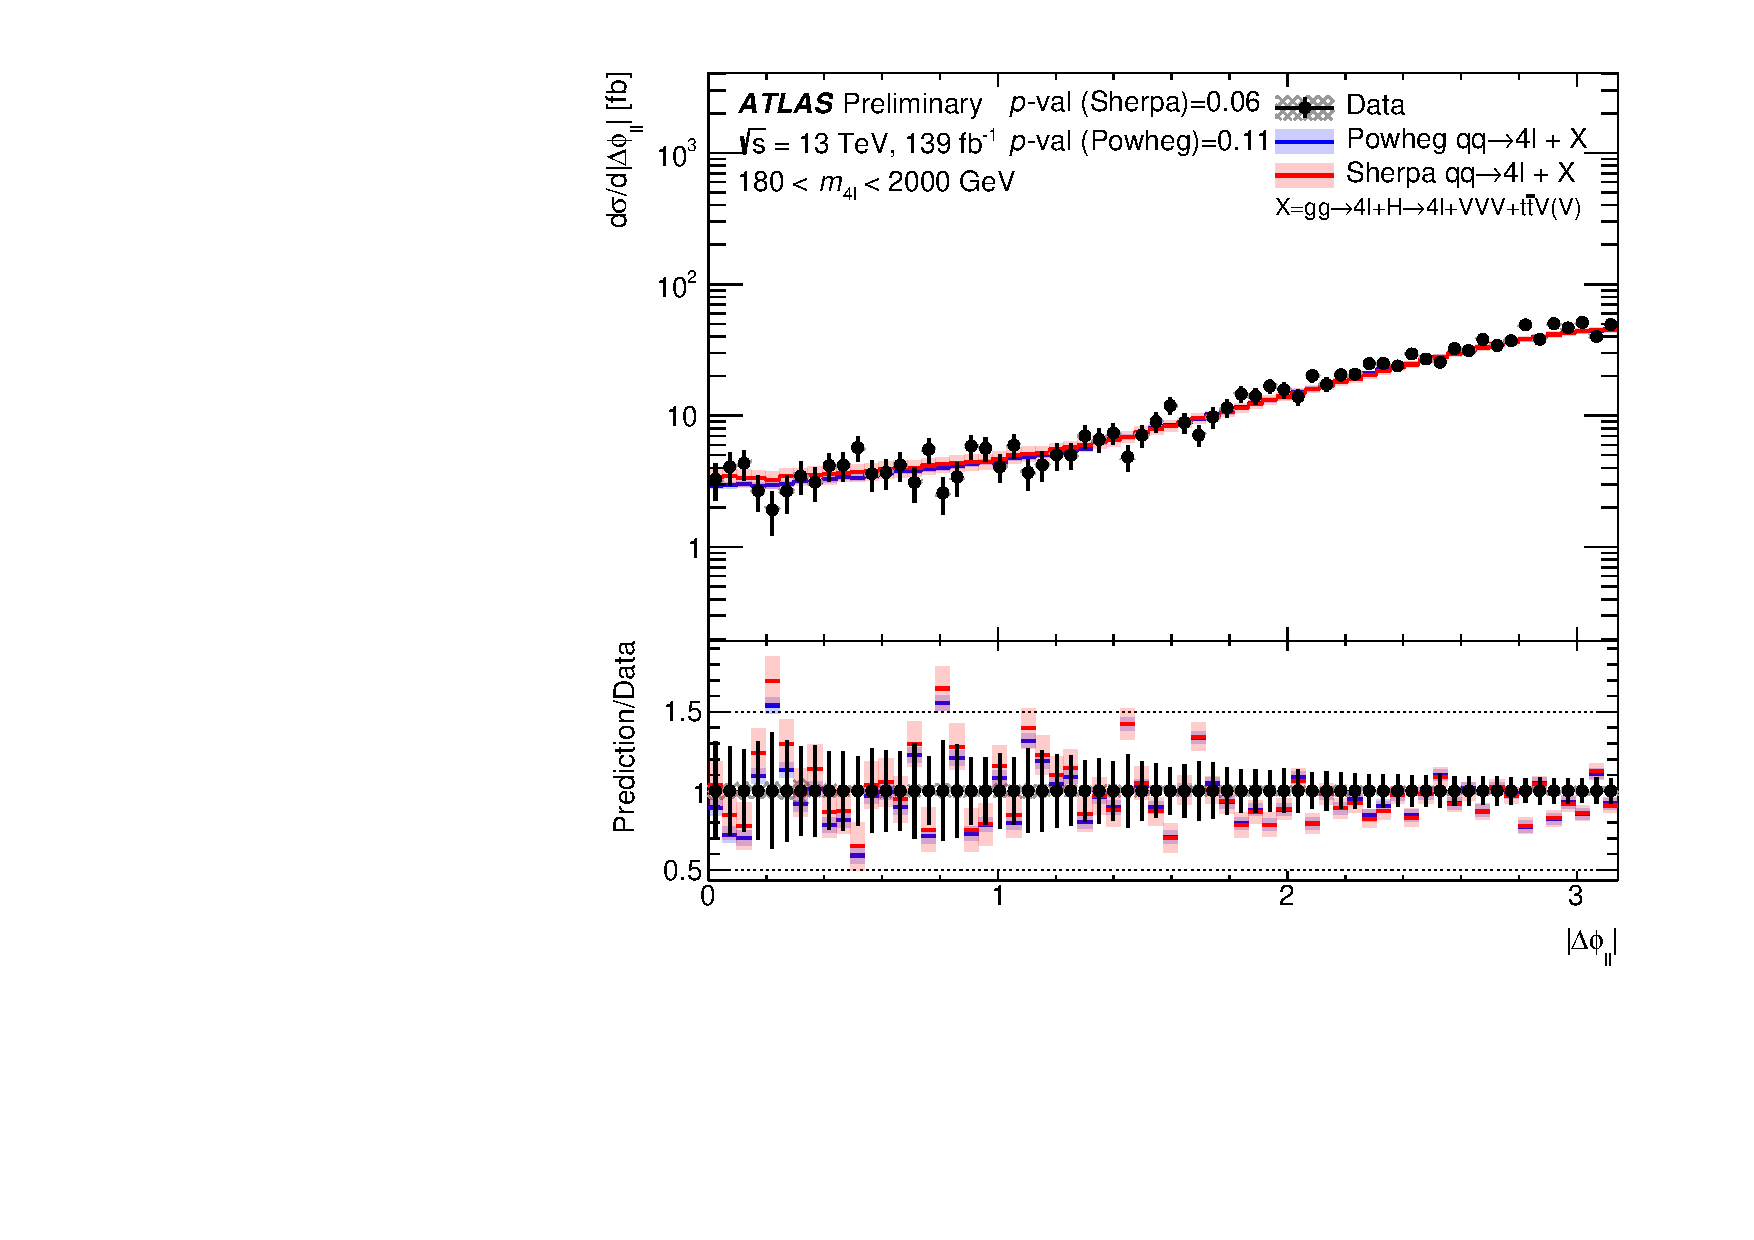
\includegraphics[width=.99\linewidth]{Figures/m4l/UnfoldedResults/Unfolded_Data_deltaPhiLeadingLeptons_m4l180-2000.pdf}  \caption{On-shell $\Z\Z$ region}\label{fig:sub-fourth}
    \end{subfigure}
    \caption{Differential cross-section as a function of \dPhill{} in the four
        \mFourL{} regions. The measured data (black points) are  compared with the SM prediction using either \SHERPA{} (red, with red hashed band for the uncertainty) or \POWHEG{} + \pythia{} (blue, with blue hashed band for the uncertainty) to model the \qqFourL{} contribution. The error bars on the data points give the total uncertainty and the grey hashed band gives the systematic uncertainty. \Pvalue{} The  lower panel shows the ratio of the SM predictions to the data.}
    \label{fig:dPhill_m4l}
\end{figure}

%% deltaPhiPairs vs m4l
\begin{figure}[htb!]
    \begin{subfigure}{.49\textwidth}\centering
      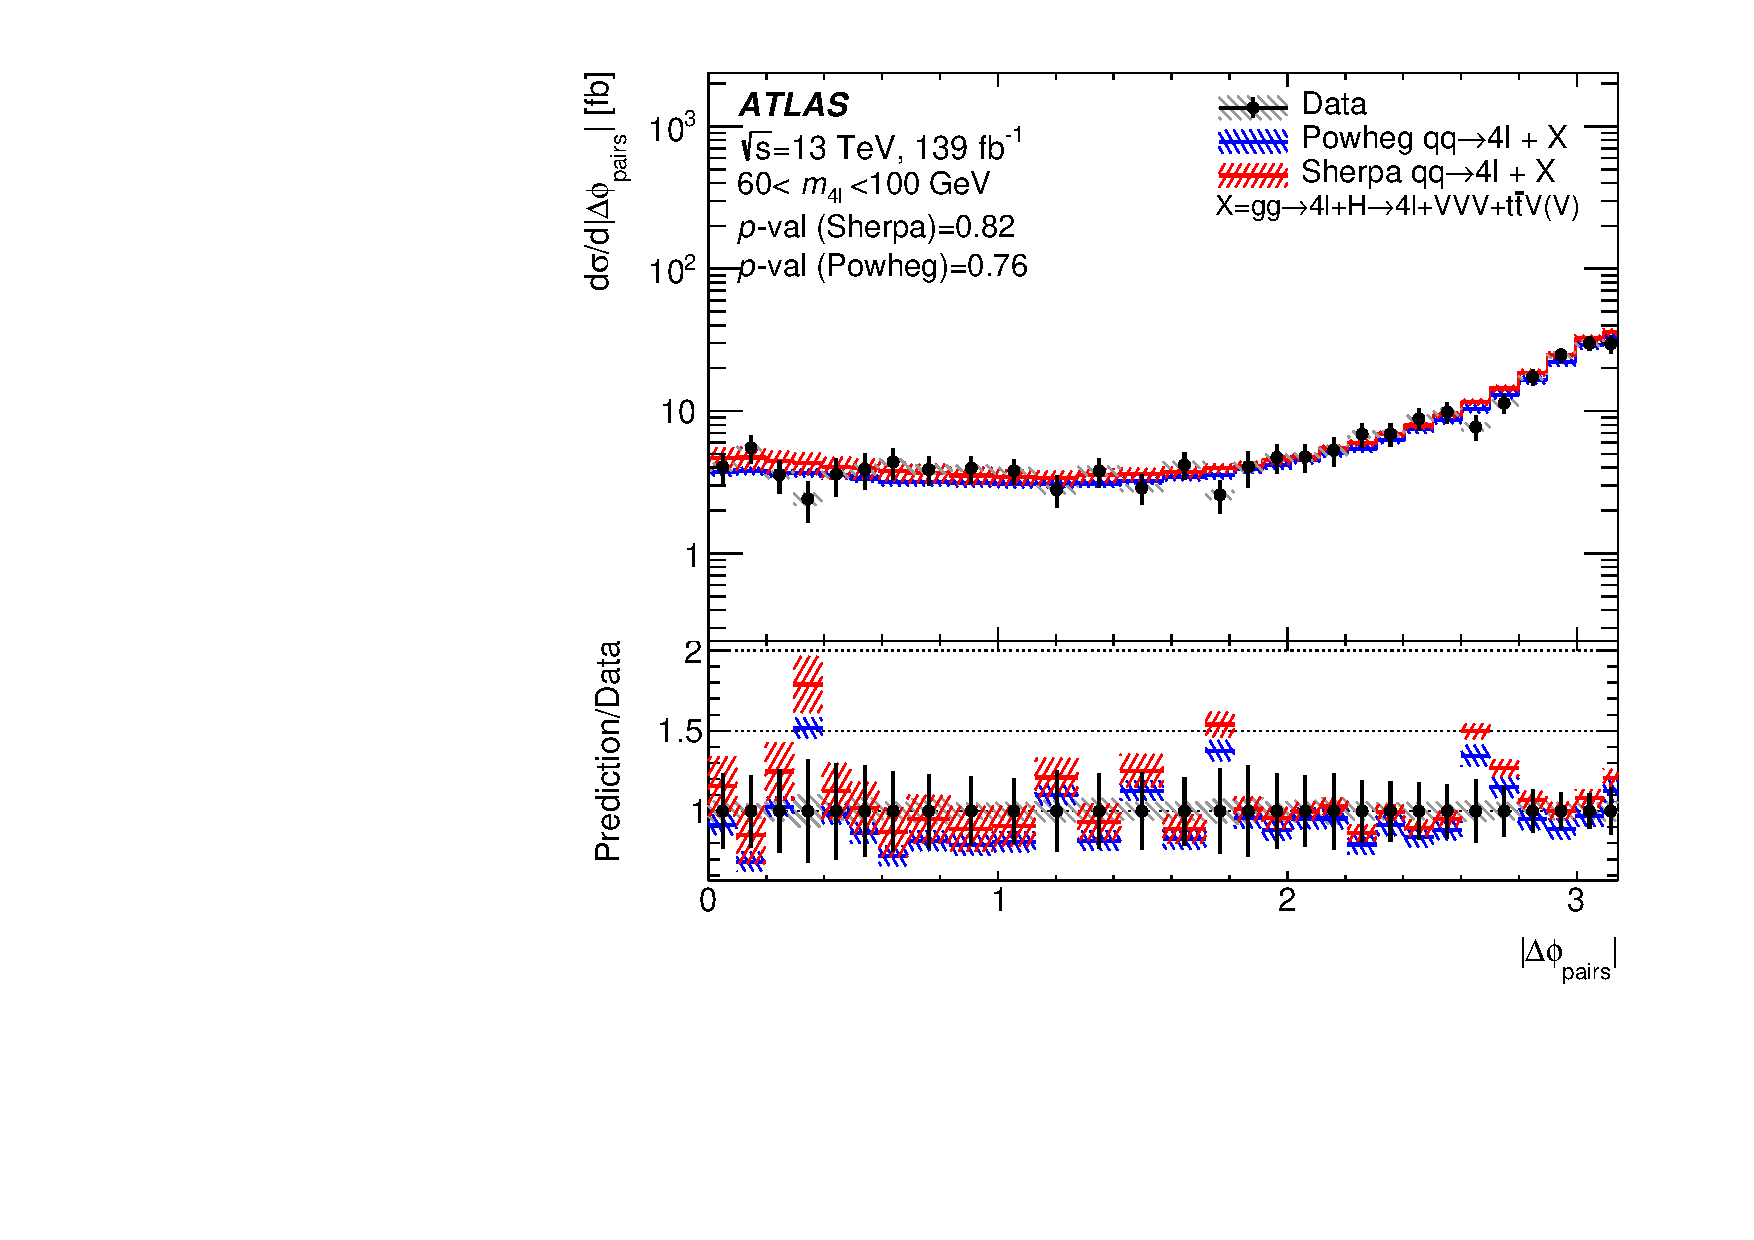
\includegraphics[width=.99\linewidth]{Figures/m4l/UnfoldedResults/Unfolded_Data_deltaPhiPairs_m4l60-100.pdf}\caption{\ZFourL \ region}\label{fig:sub-first}
    \end{subfigure}
    \begin{subfigure}{.49\textwidth}\centering
      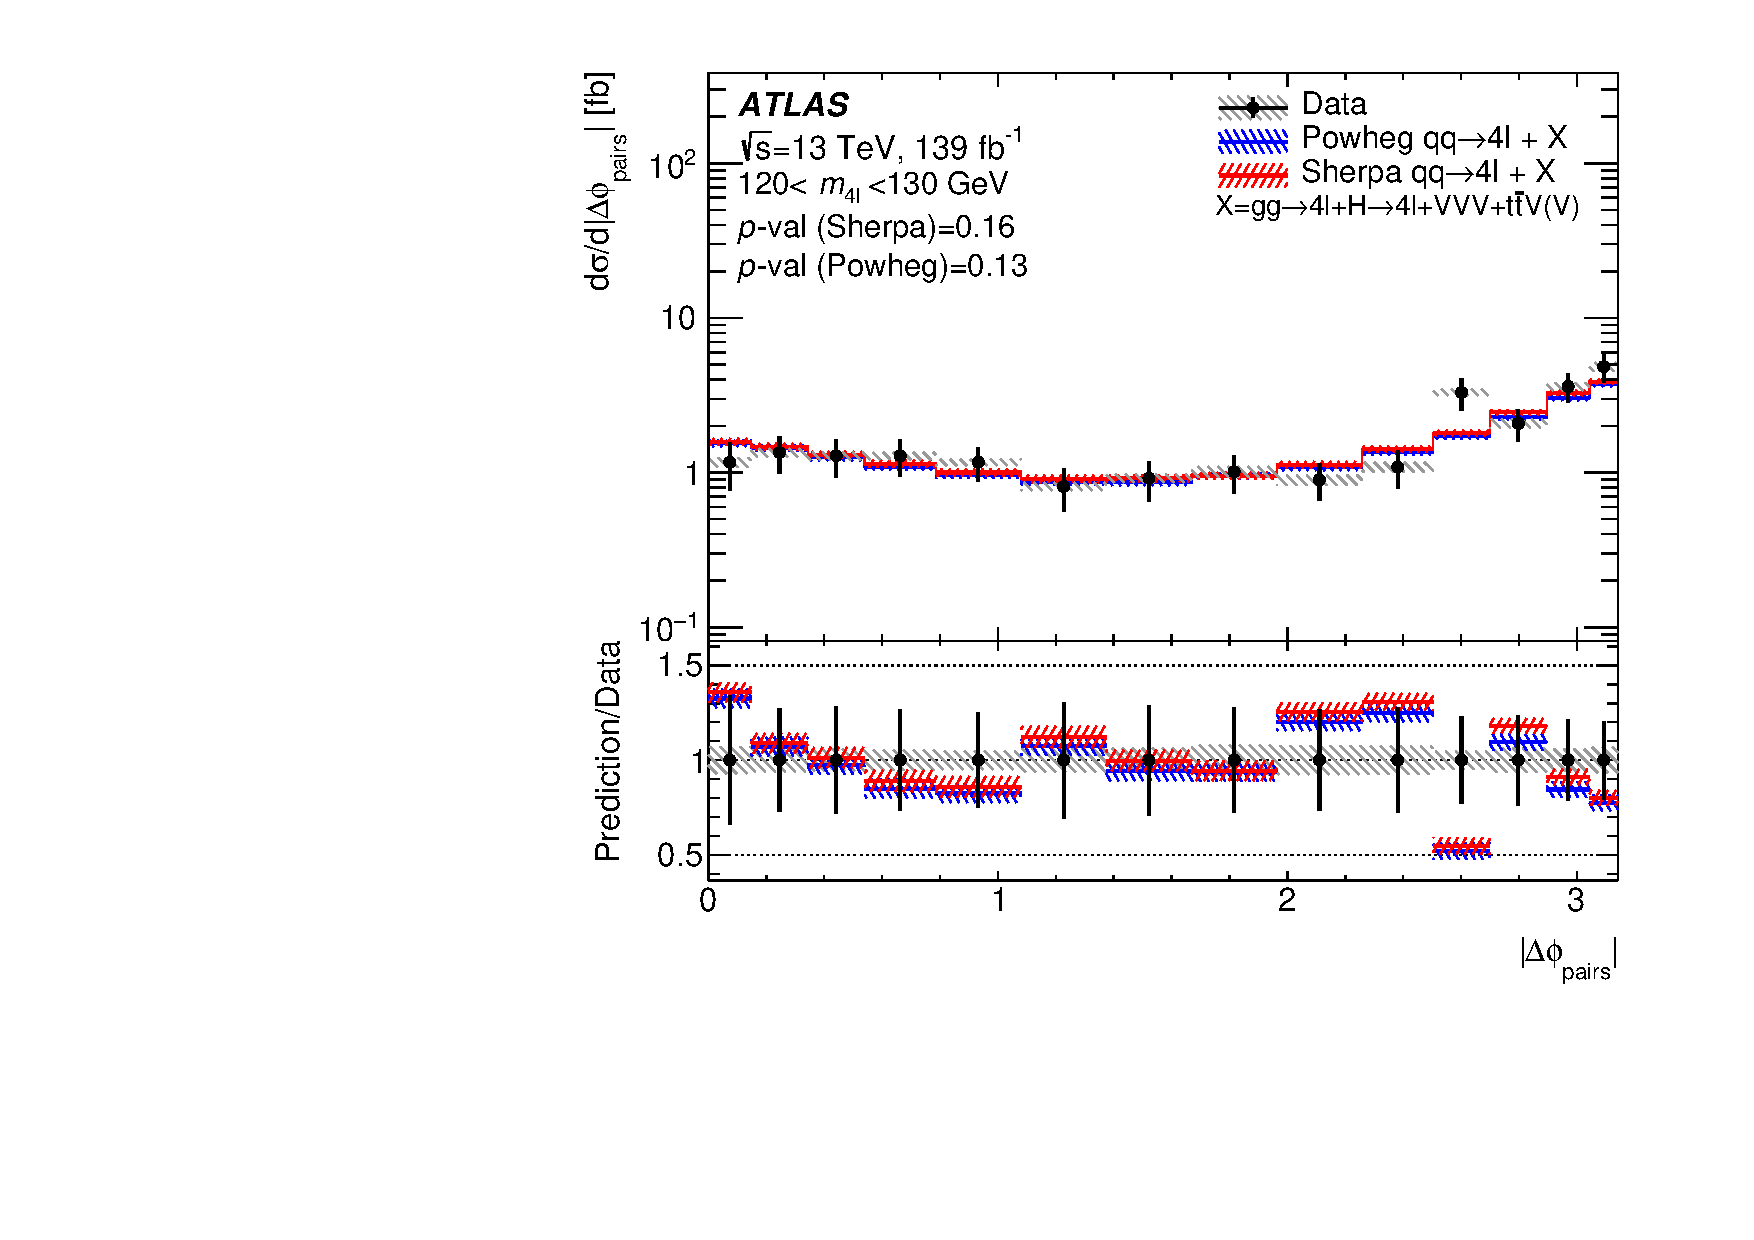
\includegraphics[width=.99\linewidth]{Figures/m4l/UnfoldedResults/Unfolded_Data_deltaPhiPairs_m4l120-130.pdf} \caption{\HFourL \ region}\label{fig:sub-second}
    \end{subfigure}
    \begin{subfigure}{.49\textwidth}\centering
      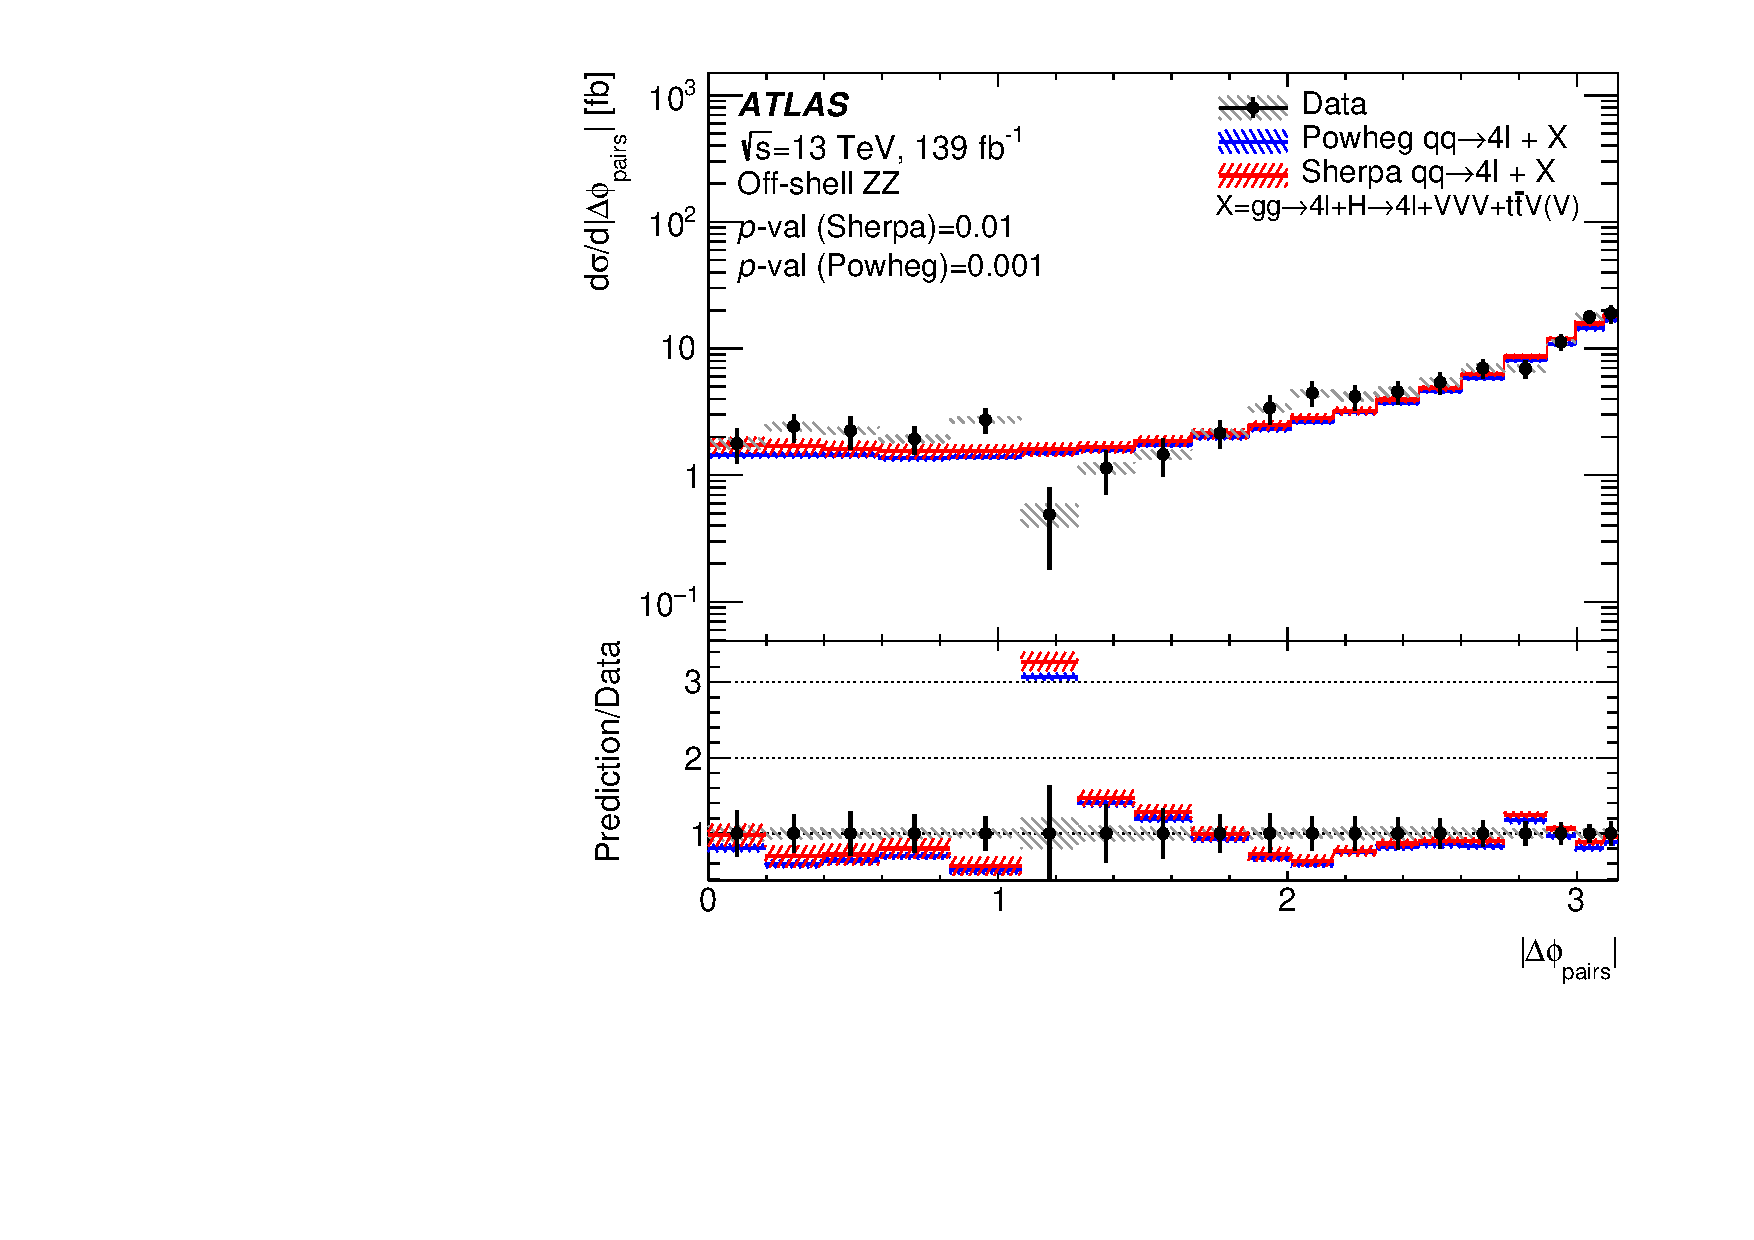
\includegraphics[width=.99\linewidth]{Figures/m4l/UnfoldedResults/Unfolded_Data_deltaPhiPairs_m4loffshell.pdf}  \caption{Off-shell $\Z\Z$ region}\label{fig:sub-third}
    \end{subfigure}
    \begin{subfigure}{.49\textwidth}\centering
      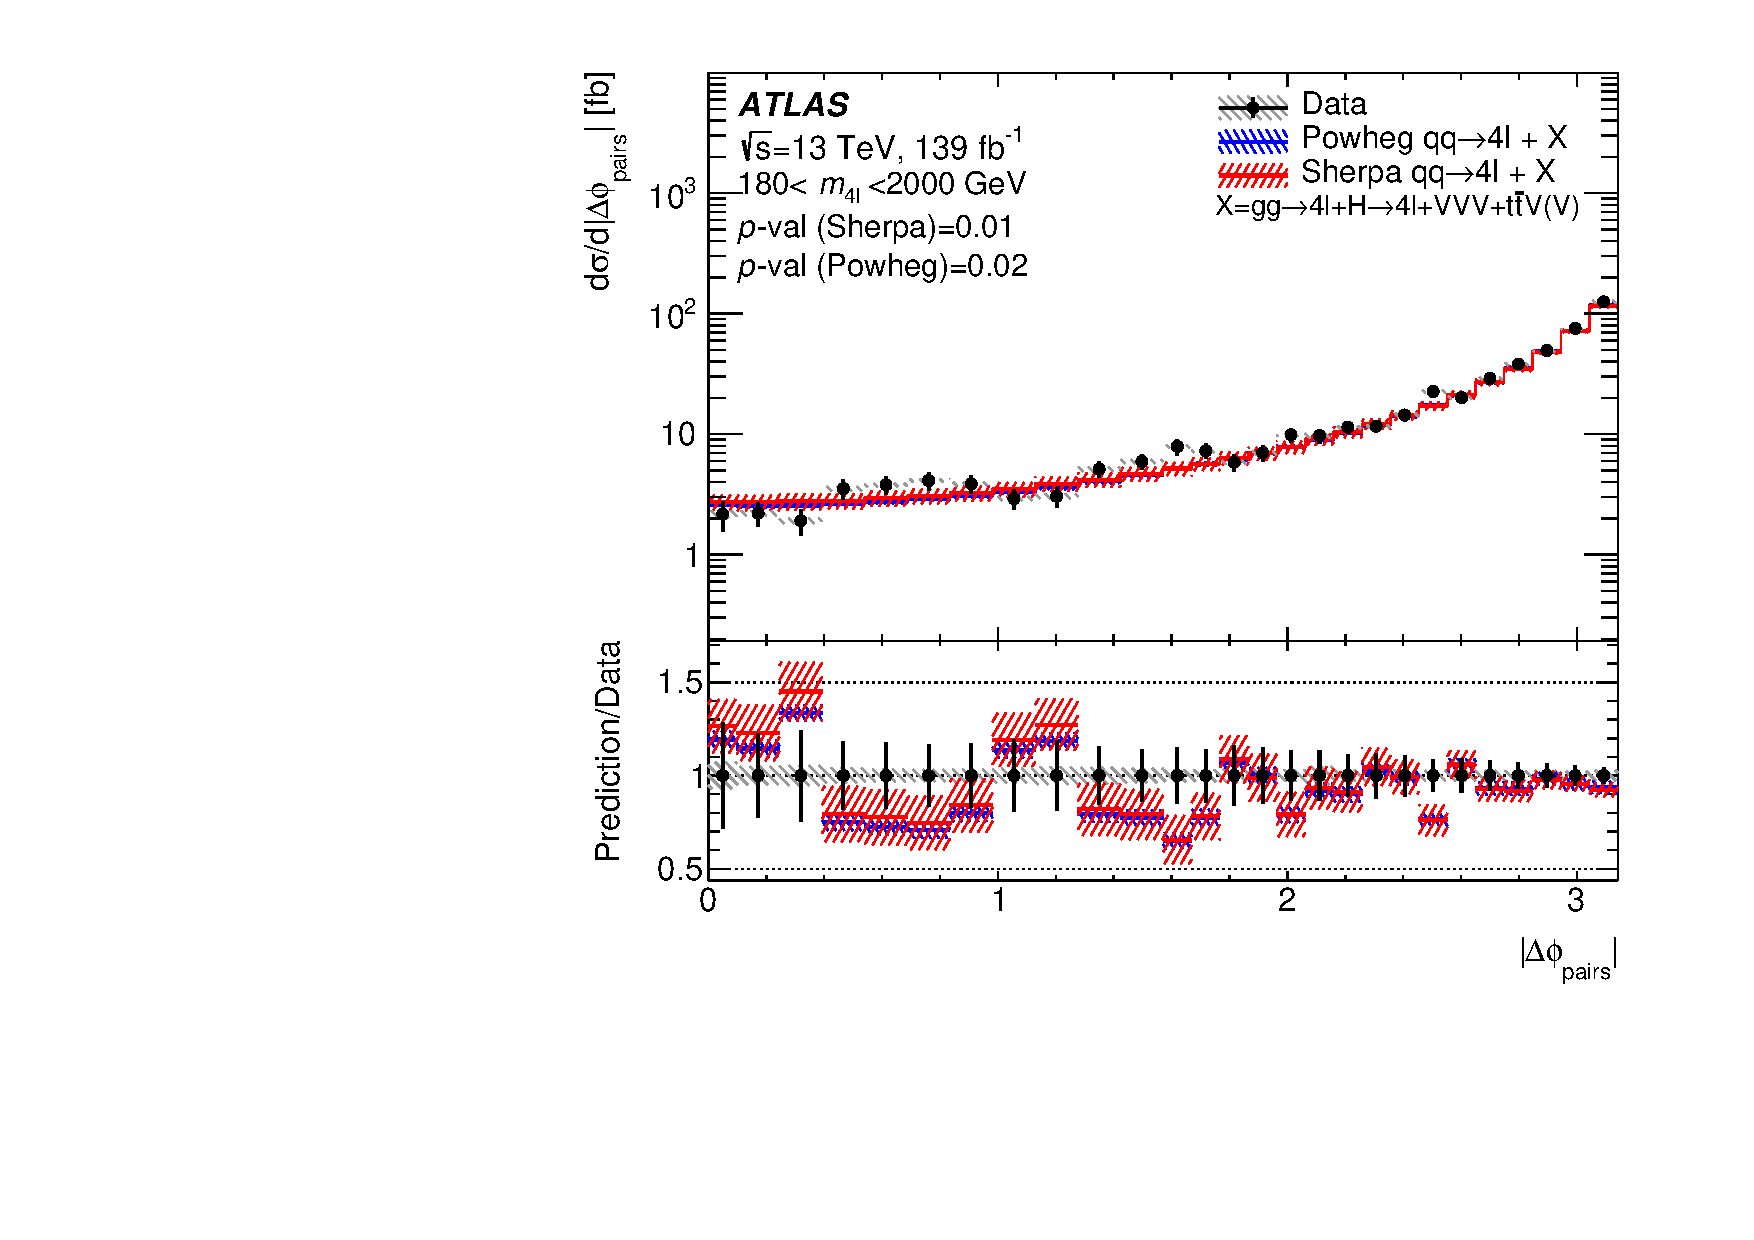
\includegraphics[width=.99\linewidth]{Figures/m4l/UnfoldedResults/Unfolded_Data_deltaPhiPairs_m4l180-2000.pdf}  \caption{On-shell $\Z\Z$ region}\label{fig:sub-fourth}
    \end{subfigure}
    \caption{Differential cross-section as a function of \dPhiPairs{} in the four
        \mFourL{} regions. The measured data (black points) are  compared with the SM prediction using either \SHERPA{} (red, with red hashed band for the uncertainty) or \POWHEG{} + \pythia{} (blue, with blue hashed band for the uncertainty) to model the \qqFourL{} contribution. The error bars on the data points give the total uncertainty and the grey hashed band gives the systematic uncertainty. \Pvalue{} The  lower panel shows the ratio of the SM predictions to the data.}
    \label{fig:dPhiPairs_m4l}
\end{figure}

%% deltaYPairs vs m4l
\begin{figure}[htb!]
    \begin{subfigure}{.49\textwidth}\centering
      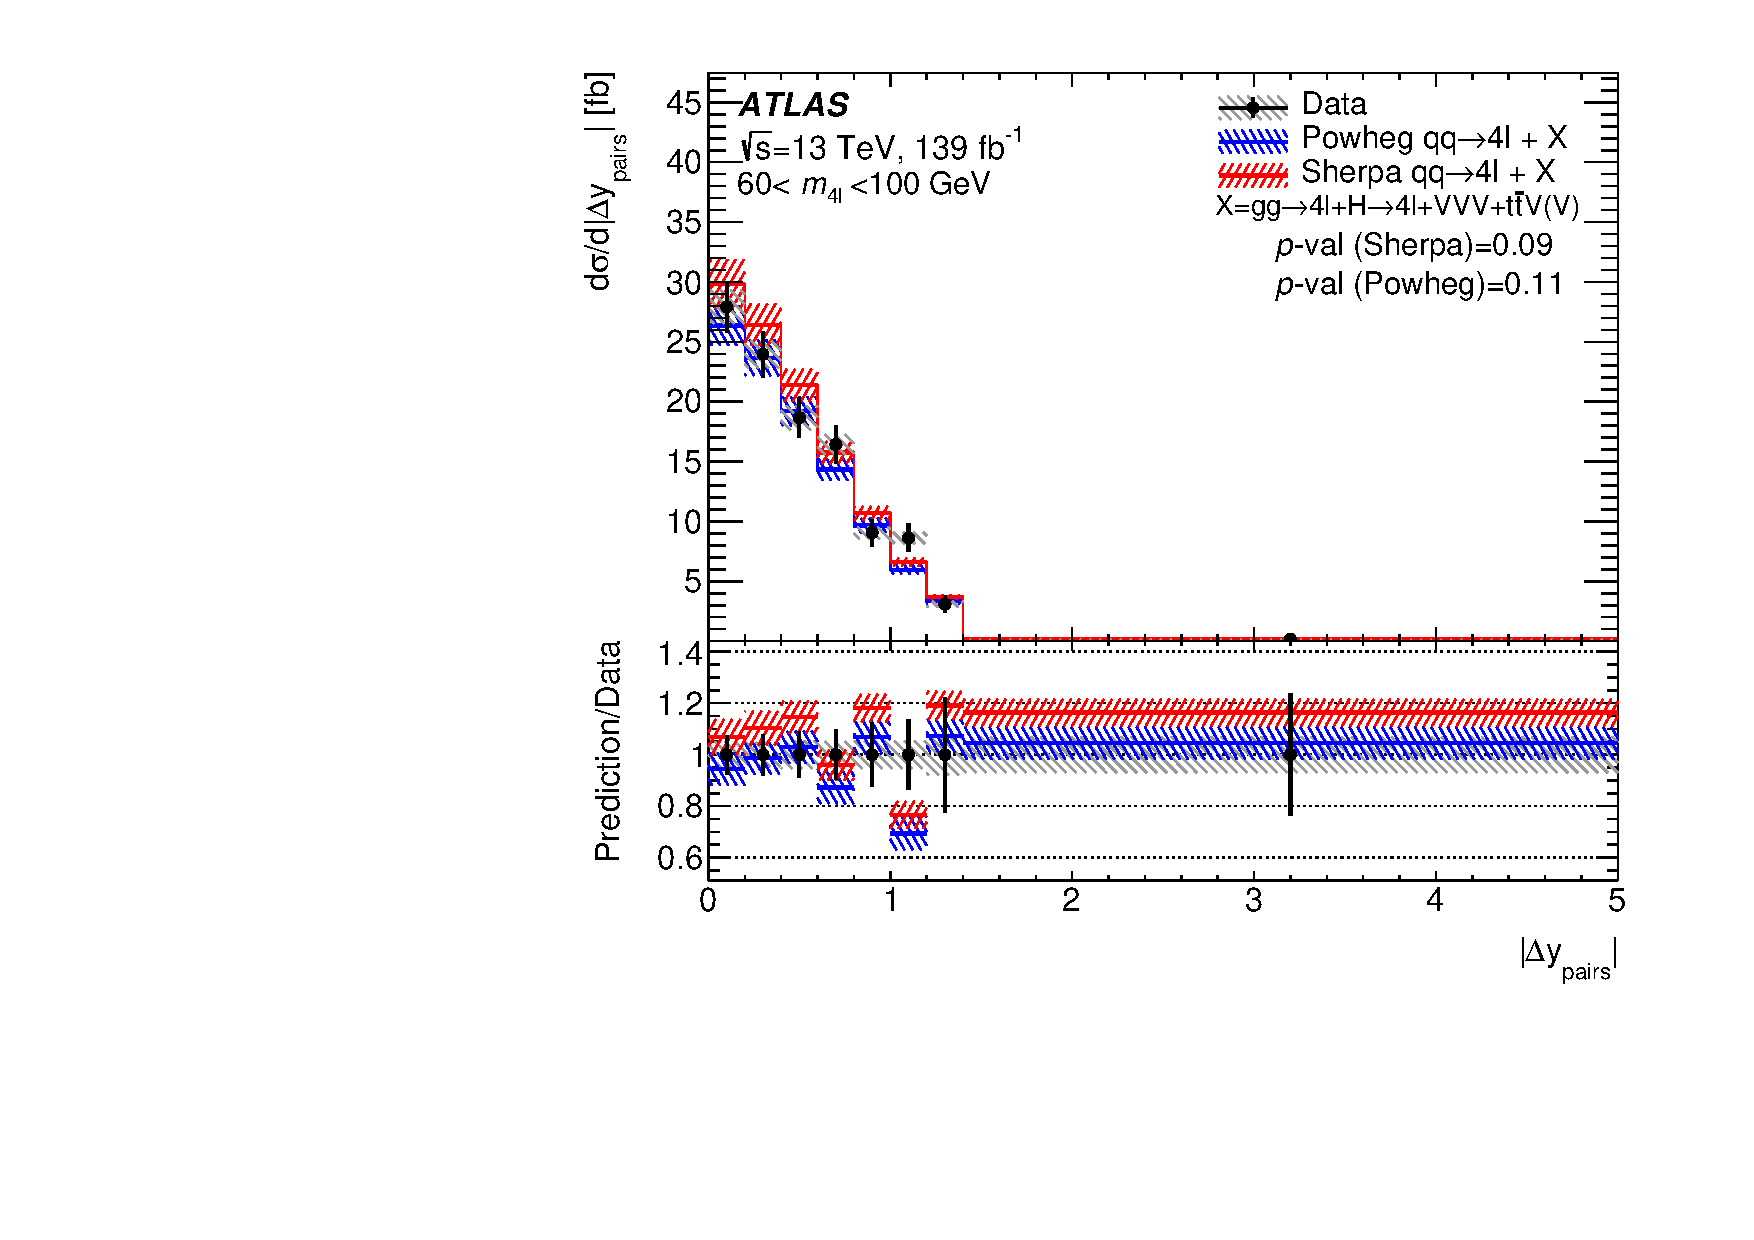
\includegraphics[width=.99\linewidth]{Figures/m4l/UnfoldedResults/linY_Unfolded_Data_deltaYPairs_m4l60-100.pdf}\caption{\ZFourL \ region}\label{fig:sub-first}
    \end{subfigure}
    \begin{subfigure}{.49\textwidth}\centering
      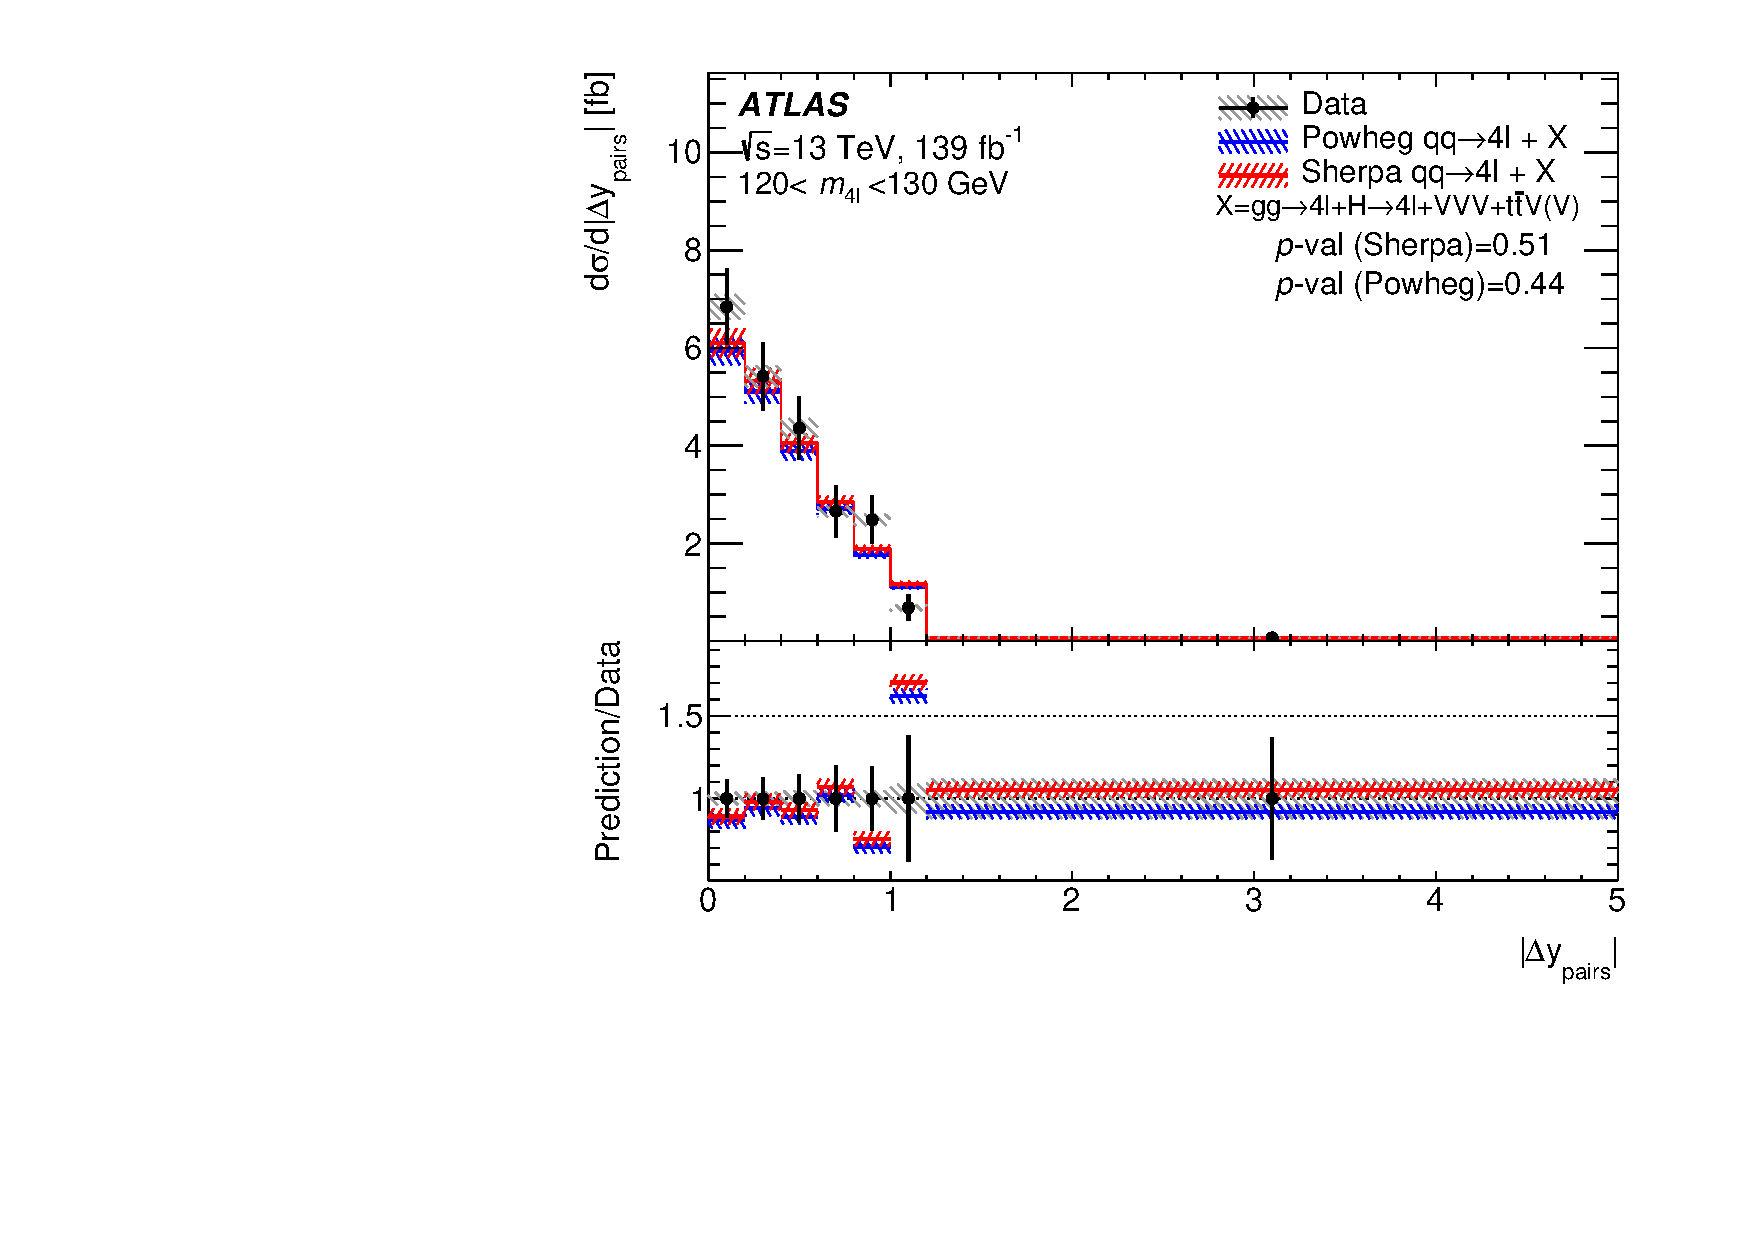
\includegraphics[width=.99\linewidth]{Figures/m4l/UnfoldedResults/linY_Unfolded_Data_deltaYPairs_m4l120-130.pdf} \caption{\HFourL \ region}\label{fig:sub-second}
    \end{subfigure}
    \begin{subfigure}{.49\textwidth}\centering
      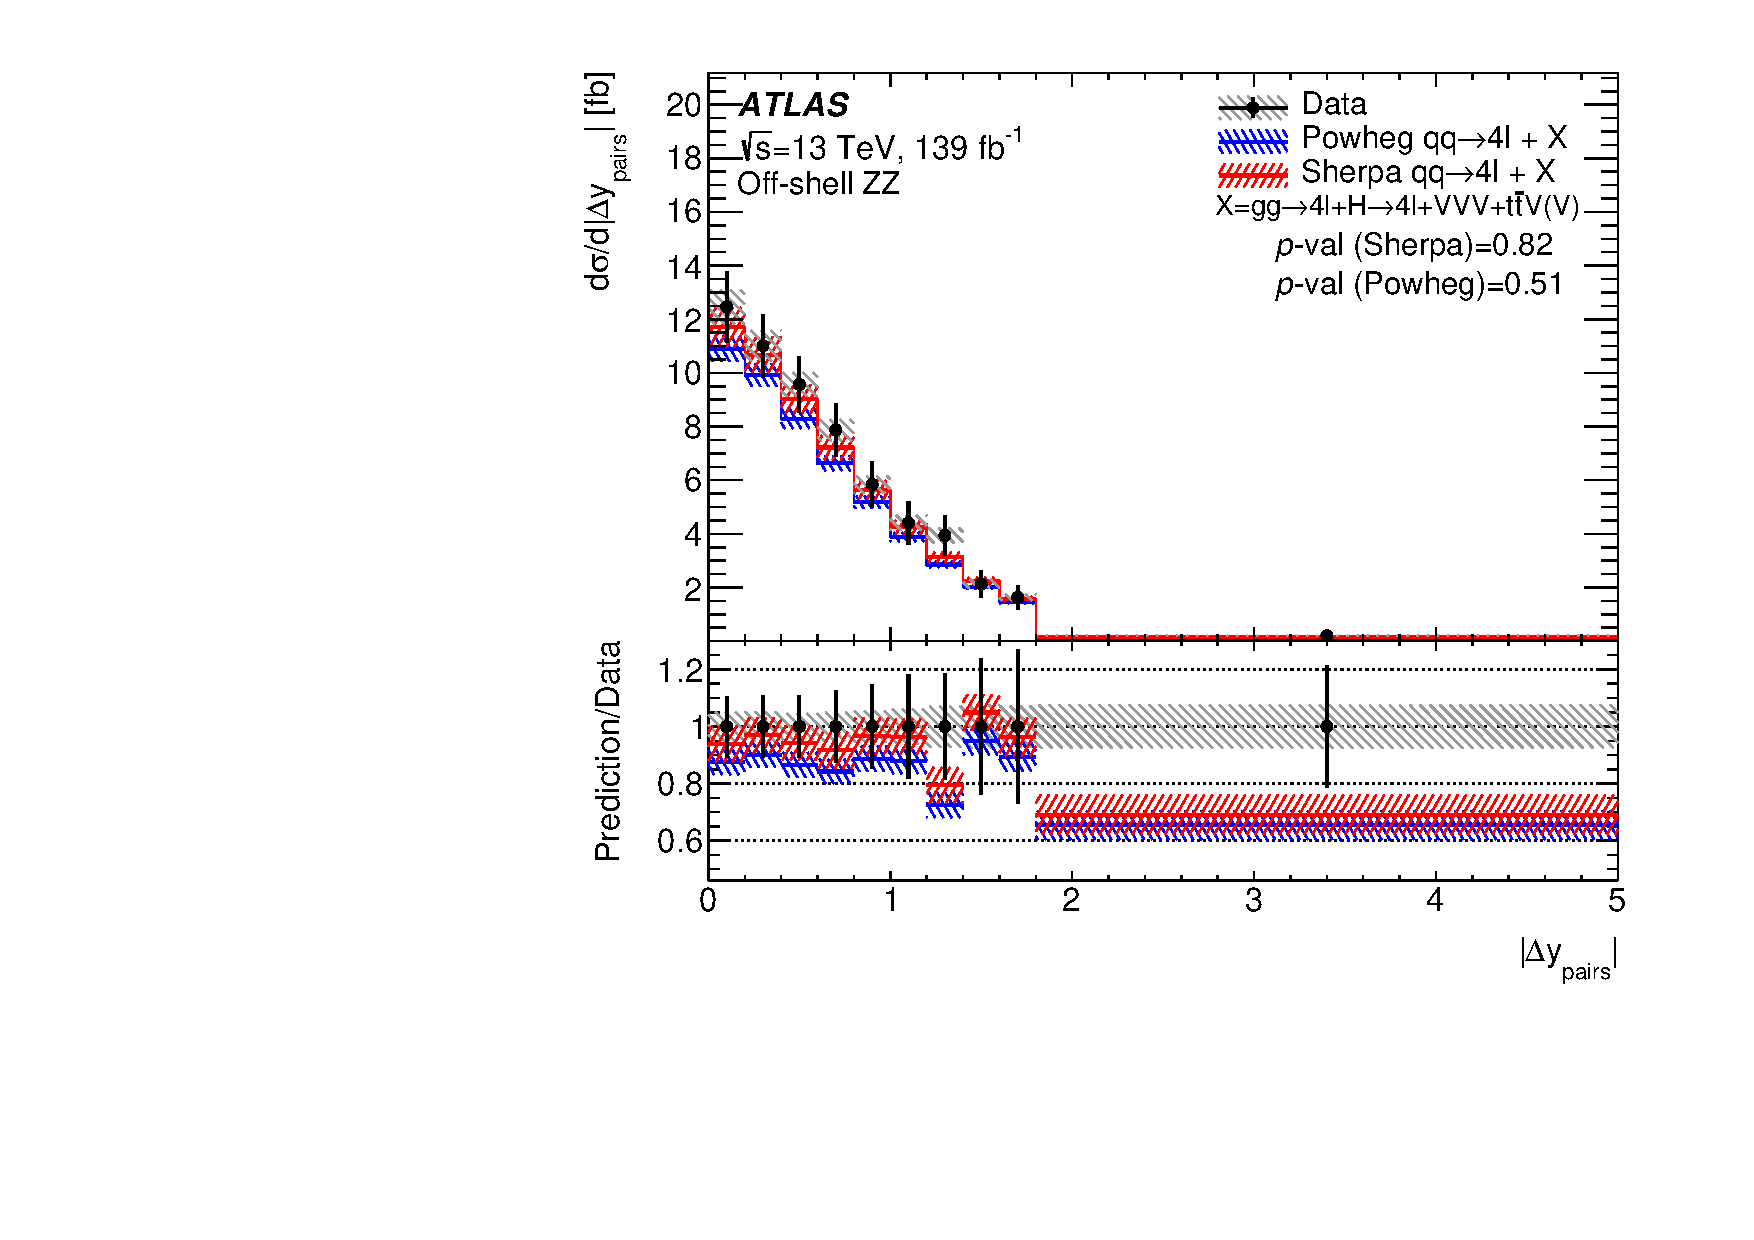
\includegraphics[width=.99\linewidth]{Figures/m4l/UnfoldedResults/linY_Unfolded_Data_deltaYPairs_m4loffshell.pdf}  \caption{Off-shell $\Z\Z$ region}\label{fig:sub-third}
    \end{subfigure}
    \begin{subfigure}{.49\textwidth}\centering
      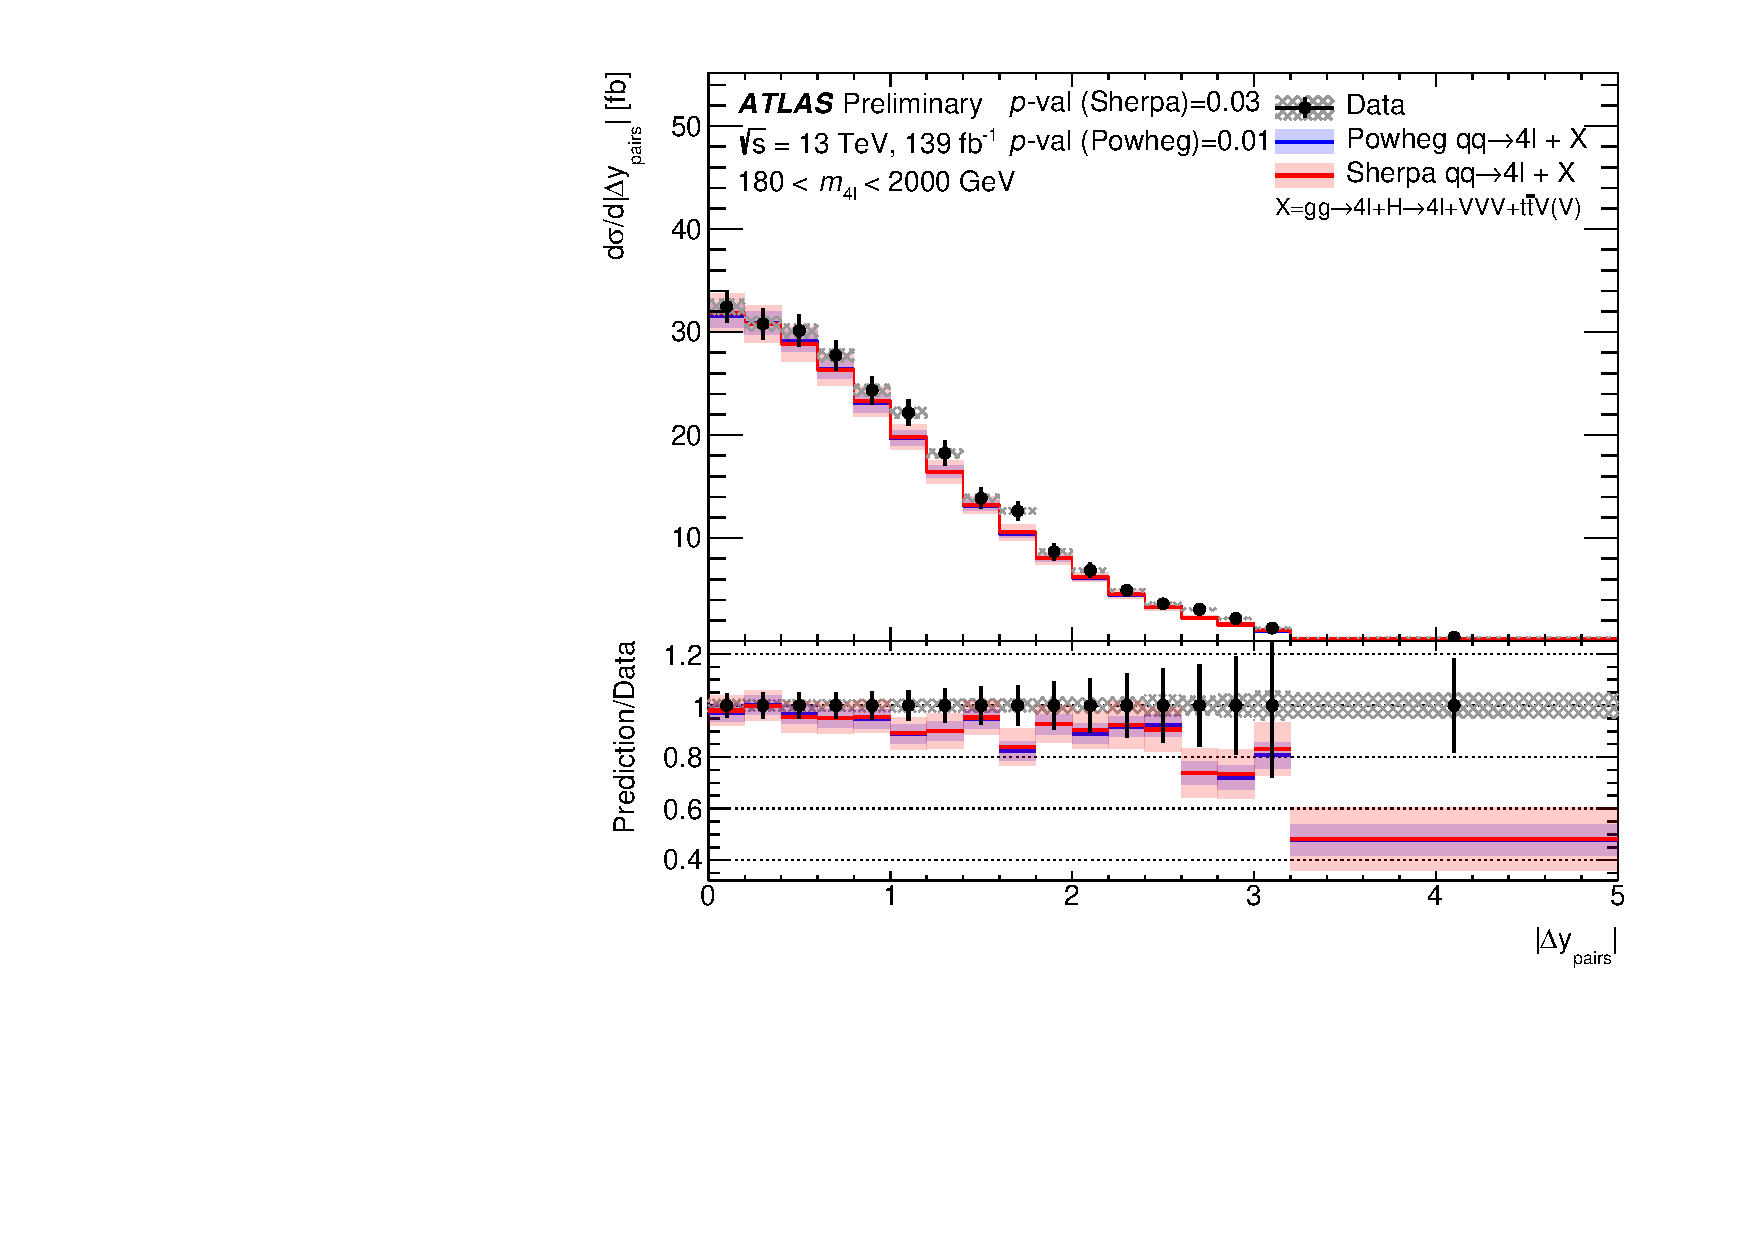
\includegraphics[width=.99\linewidth]{Figures/m4l/UnfoldedResults/linY_Unfolded_Data_deltaYPairs_m4l180-2000.pdf}  \caption{On-shell $\Z\Z$ region}\label{fig:sub-fourth}
    \end{subfigure}
    \caption{Differential cross-section as a function of \dYPairs{} in the four
        \mFourL{} regions. The measured data (black points) are  compared with the SM prediction using either \SHERPA{} (red, with red hashed band for the uncertainty) or \POWHEG{} + \pythia{} (blue, with blue hashed band for the uncertainty) to model the \qqFourL{} contribution. The error bars on the data points give the total uncertainty and the grey hashed band gives the systematic uncertainty. \Pvalue{} The  lower panel shows the ratio of the SM predictions to the data.}
    \label{fig:dYPairs_m4l}
\end{figure}